% !TeX spellcheck = es_ES


\documentclass[12pt, a4paper, titlepage,twoside,openright]{article}

\usepackage{float}
%\usepackage[spanish]{babel}
\usepackage[british,UKenglish,USenglish,english,american]{babel}

\usepackage[a4paper, top=2.5cm, bottom=2.5cm, left=2.5cm, right=2.5cm]{geometry}
\usepackage[utf8]{inputenc}
\usepackage{graphicx}
\usepackage{color}
\usepackage{hyperref}
\usepackage{longtable}
\usepackage{amsmath}
\usepackage{subfigure}
\usepackage{listings}
\usepackage{caption}
\usepackage{float}
\usepackage{algorithm}
\usepackage{algpseudocode}
\usepackage{eurosym}
\usepackage{parskip}

\usepackage{amssymb}

\setcounter{secnumdepth}{3}



\newcommand\abs[1]{\left|#1\right|}

\begin{document}

	

\begin{titlepage}
\centering		

\includegraphics[width=5cm]{Logo_URJC.png}


\vspace{1cm}

\begin{center}
	
	\Large{\textbf{Master's thesis}}
	
	%\large{\textbf{}}
	
	\vspace{4cm}
	
	\Huge
	\textbf{An hybrid architecture for multiple people tracking}
		
	
\end{center}

\vspace{6.2cm}

\begin{flushright}
	
\large


\textbf{Marcos Pieras Sagardoy}

\vspace{1.4cm}
	
\normalsize
\textbf{Móstoles, 27 de Junio de 2016}
	
	
\end{flushright}


\end{titlepage}


\tableofcontents

\clearpage



\section{Introduction}

Deep learning has rised by drastic improvements over reigning approaches towards the hardest problems in Artificial intelligence (AI), massive investments from industry giants, and exponential growth in research publications. Deep learning is a tool inside the machine learning toolbox, the goal is to make machines learn.

The first incursion was made by Frank Rosenblatt, the Percetron \cite{rosenblat}. Rosenblatt conceived of the Percetron as a simplified mathematical model of how the neurons in our brains operate. This model of the neuron built on the work of McCuloch-Pitts \cite{McCulloch}, who showed that a neuron model could model the basis OR/AND/NOT functions. Which in the early days of Artificial intelligence, was great, because the predominant tought at that time was that making computers able to perform formal logical reasoning would essentially solve AI. However, the McCuloch-Pitts model lacked a mechanism for learning, which was crucial for it to be usable for AI. This is were the Perceptron exceeled, Rosenblatt came up with a way to make such artificial neurons learn, inspirated by the Hebb's Rule. This learning method was as follows: if the output of the perceptron was low, increase the weights, otherwise decrease the weights if the output is too high. Also, another researchers came with ADALINE \cite{adaline} learning procedure, they used the signal before the activation function to compute the derivative, how much the error changes when each weight is changed can be used to drive the error down and find the optimal weights values. Similiar as we train the networks nowadays.

Researchers were really excited about this idea of Connectionism: that networks of such simple computational units could be vastly much more powerful and solve the hard problems of AI. But in 1969, Minsky and Papert  published an analysis on the limitations of perceptrons, named Perceptrons \cite{minsky69perceptrons}. The biggest criticism was that a pereceptron could not learn the simple boolean function XOR because it is not linearly separable. However, they stated that it could be learnt with multiple layers perceptron but the learning procedure did not work for multiple layers. After, this book the interest on Neural networks decreased, and initlizate a period called \textit{AI winter}, AI shifted to logic programming and commonsense reasoning.

This period lasted till 1986 when Rummelhart, Hinton, and Williams published the algorithm of backprogation \cite{Rumelhart}, which specifically adressed the problems discussed by Minsky in Perceptrons, a method to train multiple layer neural nets. With this discovery in 1989, LeCun showed a real world application, recognized handwritten digits \cite{lecunZip}. The architecture of this model was a convolutional neural network. It was inspired by the Neurocognitron \cite{Fukushima} of Fukushima, which took ideas from studies of the brain. In particular the studies of Hubel and Wiesel, they propose that the visual cortex is formed by a hierarchical model, primarilly for simple cells who respond for simple structures and then complex cells respond to a more complicated feature. As we can observe in figure \ref{intro1}, in the lower layer, the network learns Gabor like features, and while going upwards, the networks learns more abstract concepts.




\begin{figure}[H]
\centering         
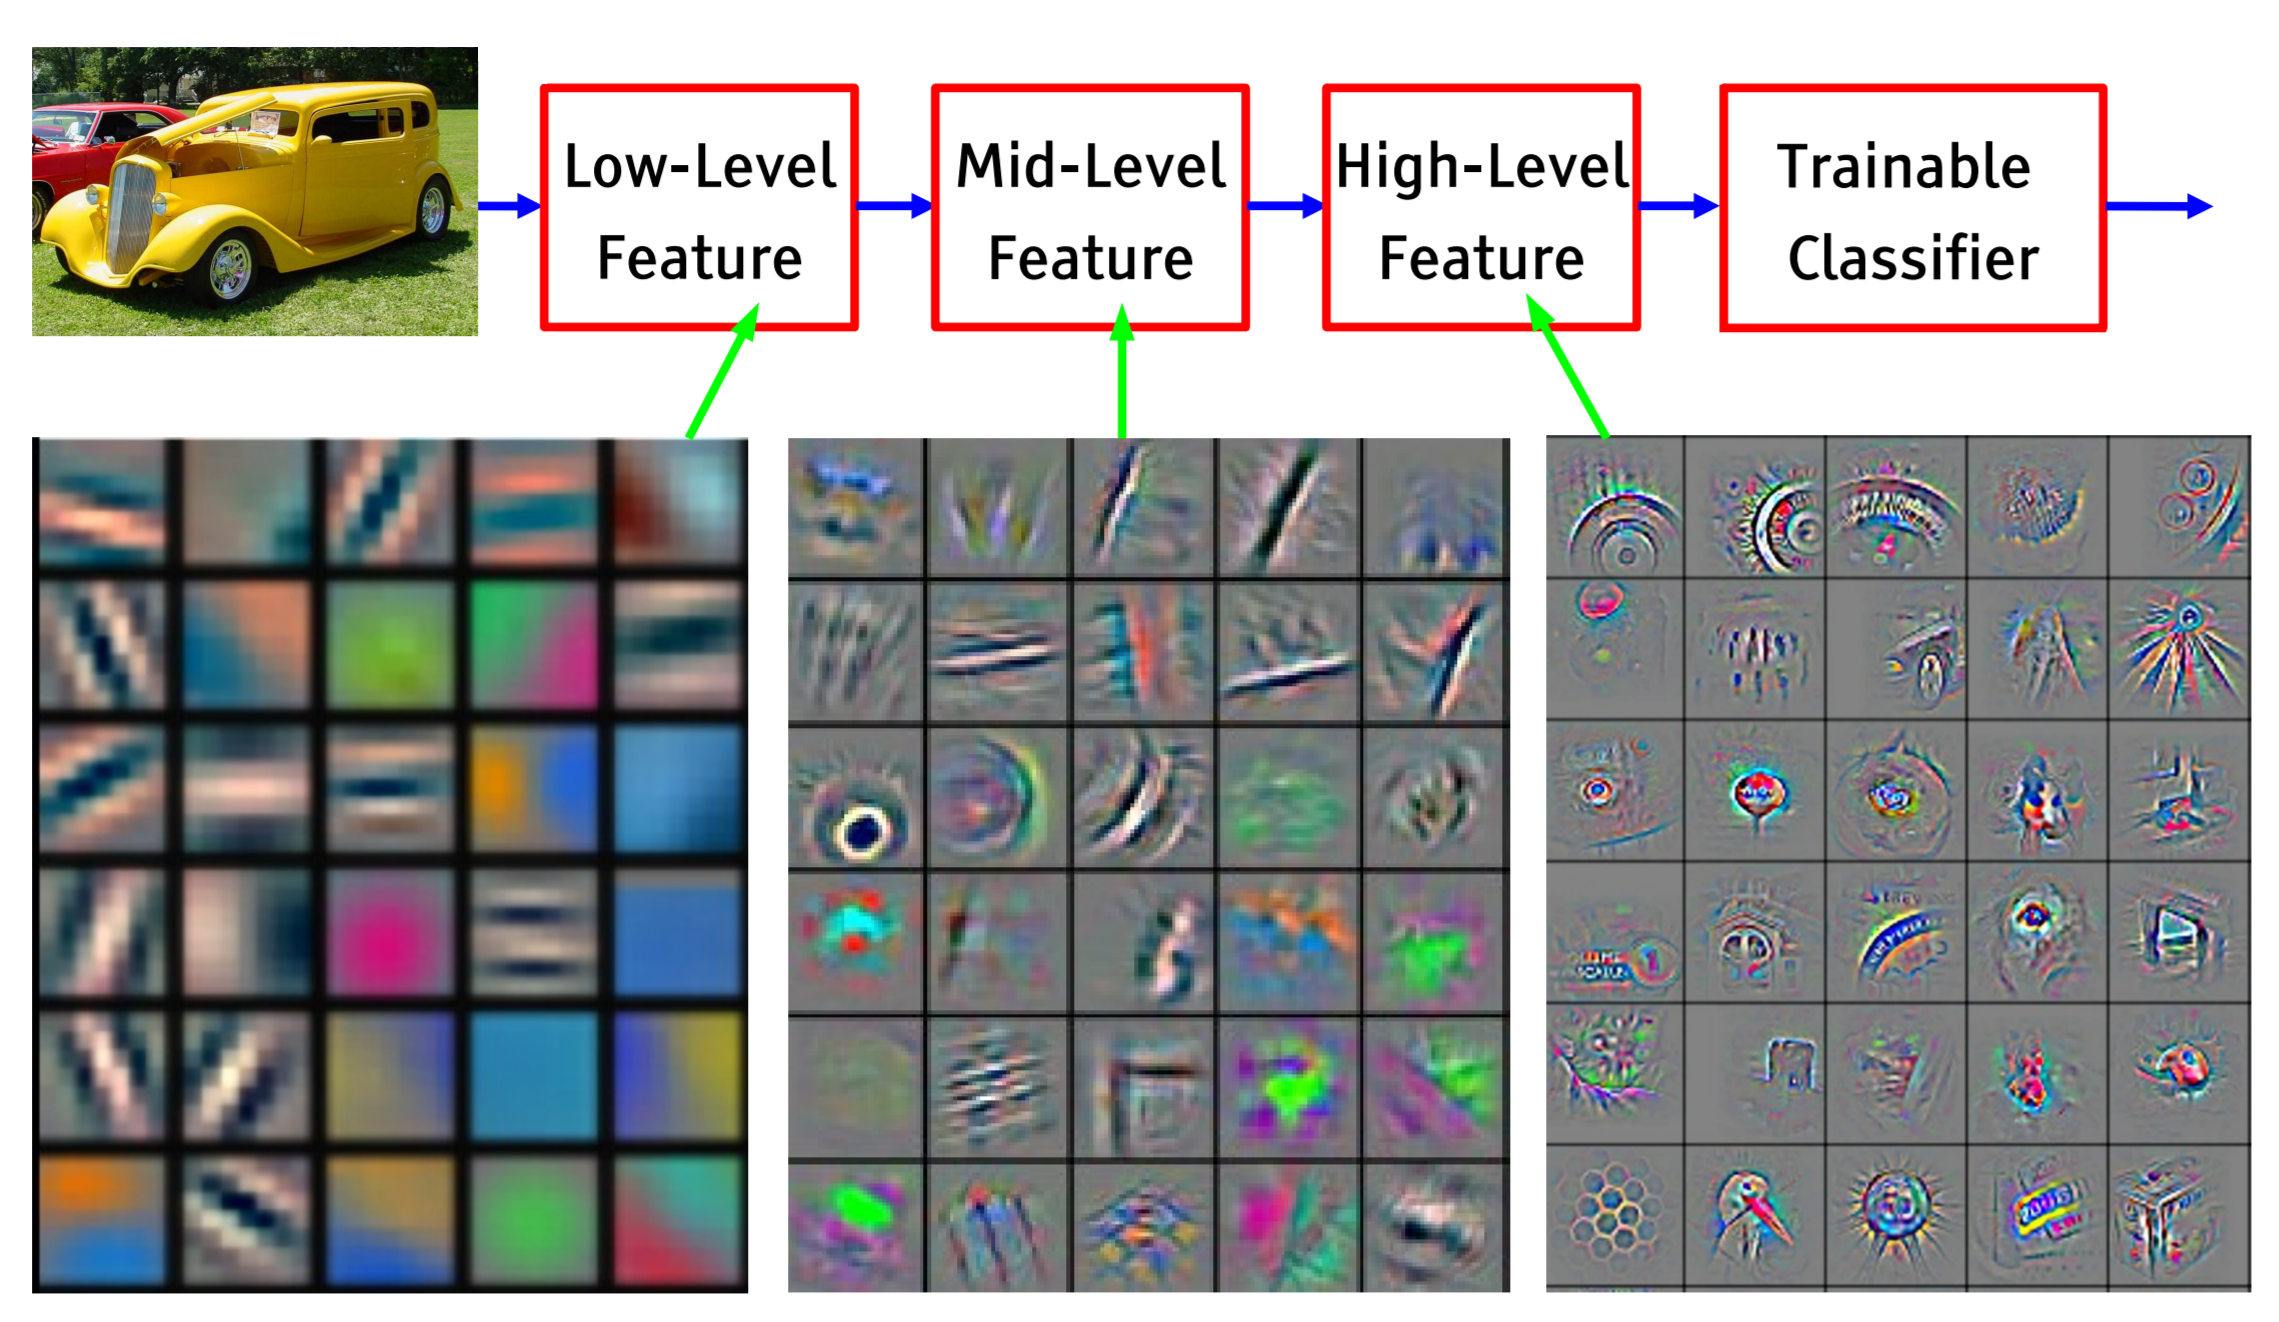
\includegraphics[width=12cm]{intro/model.png}
\caption{Representation of a Convolutional neural network.} \label{intro1}
\end{figure}



But this approach did not scale to larger problems, the biggest source of problems was the vanishing gradients problem. When the backpropagtion gradients backpropagets trough the network, in some nodes the local gradient is very low ( in the extreme of the sigmoid functions ) the signal vanishes or saturates, and by the 90s other techniques became the method of choice, like support vector machine (SVM). Altough some progress was made for other kinds of problems.

\begin{itemize}

\item Unsupervised learning. This types of architectures are used to finding a smaller representation of some data from which the original data can be reconstructed, it is useful for compression, visualization, and classification. One example of this architecture with neural networks, is the Restricted Boltzman machine \cite{boltzmann}, developed by Hinton.
%in this setting the neurons behave according to a probability distribution, and form a graphical model. The neuron are hidden %layers, and it can be used to infer information from it.
 
\item Reinformcent learning. The goal of this type of learning is to learn how to make good decisions, it requires rewards, not labels. One example of this sort of systems, is the TD-Gammon \cite{Gammon}, a neural network that learned to be a backgammon player.

\item Robotics. This was another field separate from Machine Learning where neural nets were very useful. A major example of early neural net use for robotics came from CMU's NavLab in 1989. the neural net learned to control the vehicle using steering data recorded while a human drove \cite{alvin}.

\item Recurrent neural networks. Plain neural networks could not process sequences due to they do not have memory, they need mechanism to remmeber the pasts ouputs. With memory, it can process sequences like audio or text. One approach to this, by Waibel \cite{Waibel} in 1989. 


\end{itemize}


In 2006, there was a breaktroguht \cite{hinton06}, Hinton realized that a neural network with many layers really could be trained well, if the weights are initilzaized in a clever way. The basic idea was to train each layer one by one with unsupervised training ( like an autoencoder architecture ) and finally stack all together and train it in a supervised way. But the big breaktrought came in 2012, when a neural network won the Large scale visual recogntition challenge.



% http://nautil.us/issue/21/information/the-man-who-tried-to-redeem-the-world-with-logic
% http://beamandrew.github.io/deeplearning/2017/02/23/deep_learning_101_part1.html
% http://pijamasurf.com/2017/05/aprender_cine_mirando_cine_15_peliculas_para_iniciarse_en_la_apreciacion_cinematografica/


% http://nautil.us/issue/21/information/the-man-who-tried-to-redeem-the-world-with-logic



%Deep learning allows computational models that are composed of multiple processing layers to learn representations of data with multiple levels of abstraction. Traditional methods relay in hand-crafted ( also called engineered ) features to build a representation of the instance, and then learn a predictor to inference some label about it. These features are made by an expert to highlight the parts that they thought it could be more discriminative. Later on, the community applied the kernel methods, this methods try to find discriminability increasing the dimensionality of the features. In contrast, deep learning techniques, features are learned from the raw data and also are deeper than the hand-crafted features and kernels, therefore allows to compute more intrinsic properties. In the figure \ref{deepEsquem} we summarizzes the differences.
%
%
%
%\begin{figure}[H]
%\centering         
%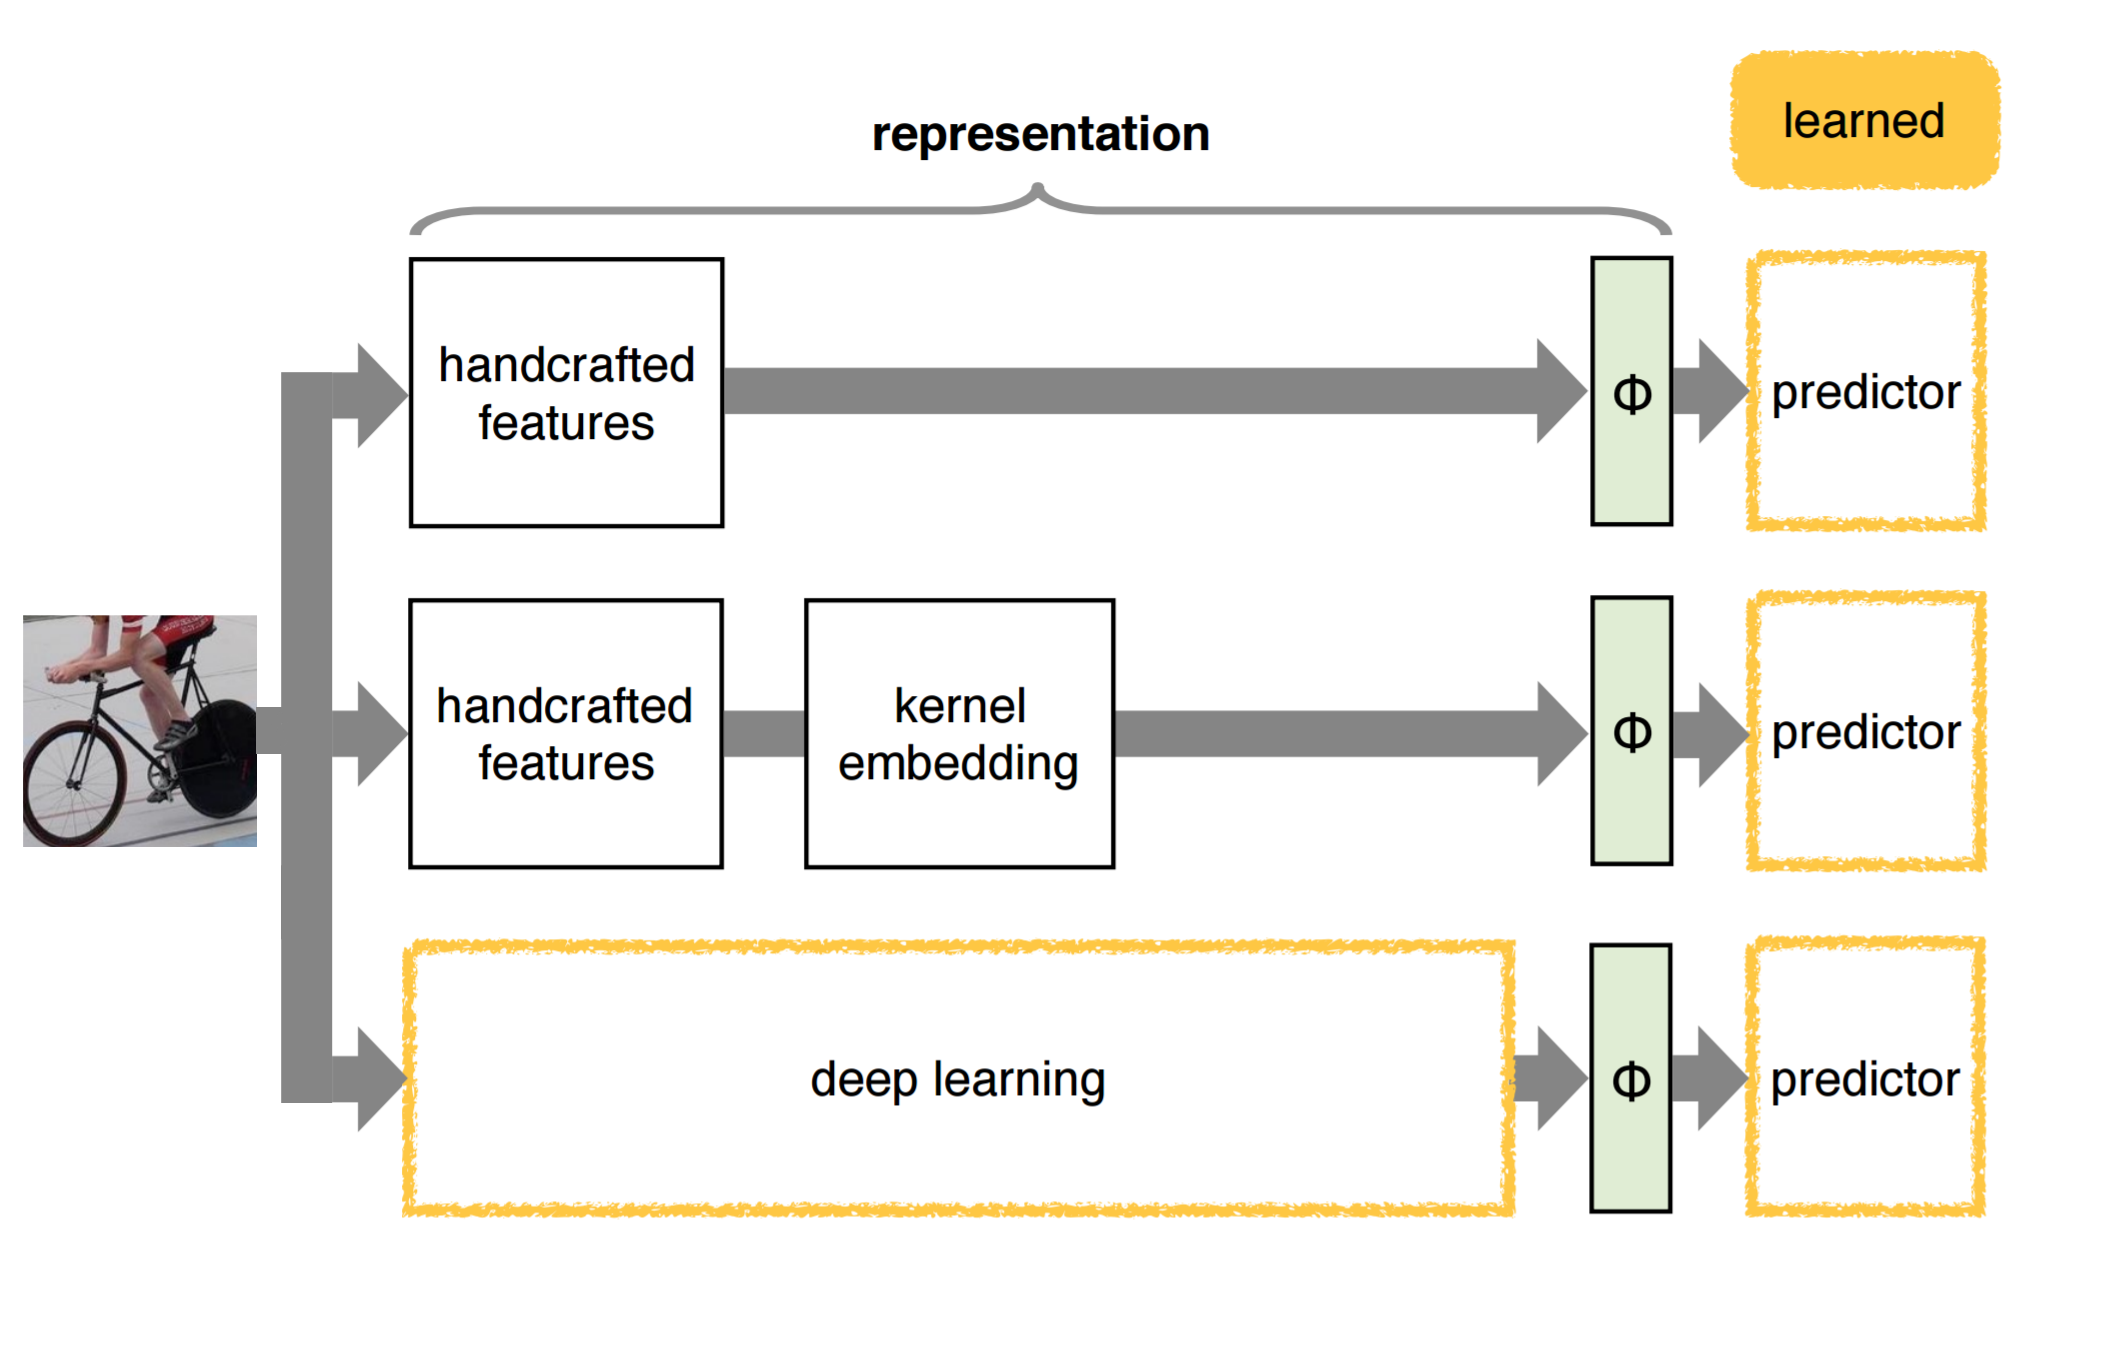
\includegraphics[width=0.6\linewidth]{objectDetection/esquema2.png}
%\caption{Comparision between traditional and deep learning methods.} \label{deepEsquem}
%\end{figure}



Although, this improvements, the big breaktroguht came in 2012, when AlexNet \cite{alexnet} beat the state of the art in the ImageNet challenge, an image classification challenge, where the error rate was $15.3 \%$ whereas the winner of the previous year was $26.3 \%$. In the plot \ref{intro2} we can observe the advance in the state of the art of the ImageNet challenge with the inclusion of deep learning techniques.




\begin{figure}[H]
\centering         
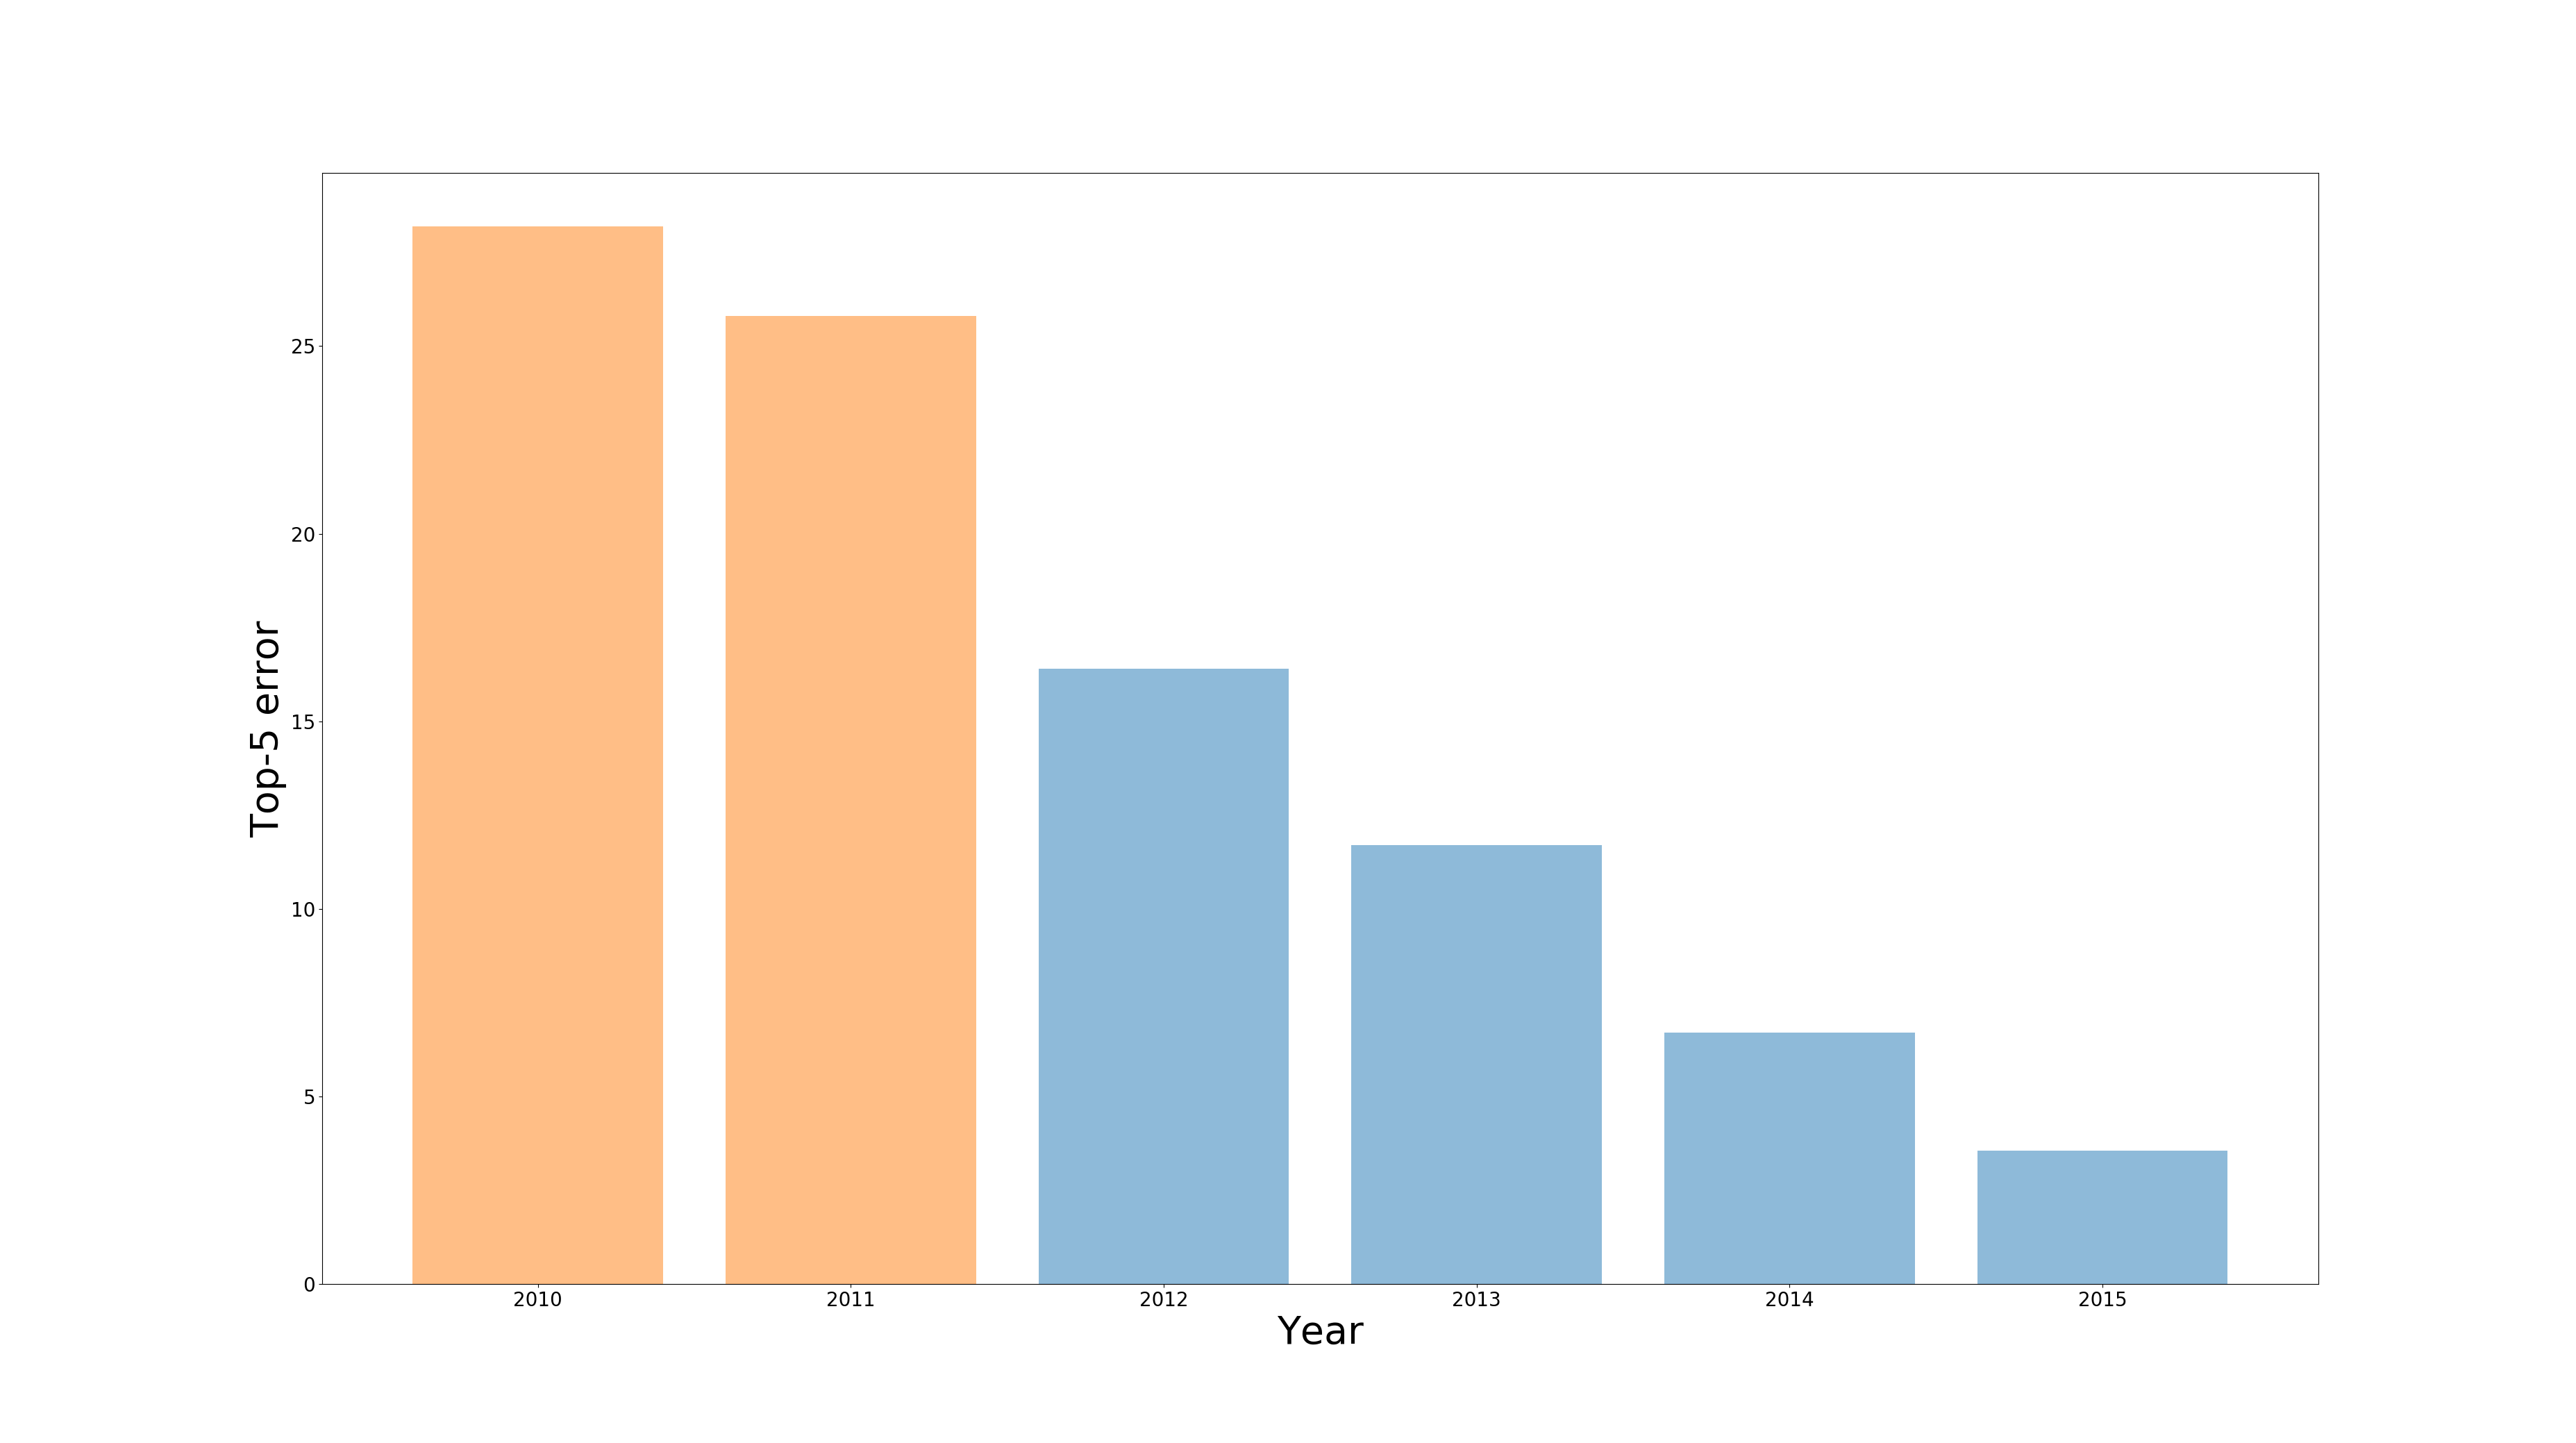
\includegraphics[width=0.7\linewidth]{intro/iamgeWihtou.png}
\caption{Classification error in ImageNet challenge.} \label{intro2}
\end{figure}



The emergence of these techniques were the culmination of decades of research but the step forward was dued by three aspects:

\begin{itemize}

\item \textbf{Appearance of large and high quality dataset}, The increasing size and quality of the dataset helps the networks to converge easily.

\item \textbf{Parallel computation}, The increasing of computing capabilities helped train larger models in least time.

\item \textbf{Optimization details}. With the discovery of the proper inizialization and activation functions larger networks can be trained.


\end{itemize}


\subsection{Tracking with deep learning techiniques}

As we said above, Deep learning techinques has increased the perfomance in all the aspects of computer vision, as well as Tracking, the main ways to apply deep learning techniques to tracking are the following \cite{thrun}:

\begin{itemize}


\item \textbf{Online training for tracking}. Starting from the first frame of a video, a tracker will sample patches near the target object, and they are used to train a foreground-background  classifier, and this classifier is used to score patches from the next frame to estimate the new location of the target object. These methods showed a state-of-the-art perfomance results. Unfortunately, neural networks are slow to train, therefore the speed of the method is reduced \cite{deep1} \cite{deep2}.

\item \textbf{Model based trackers}. These methods use a specific class classifier and there is not need to train it online. So, these methods use a neural network to extract instances of the frames and then linked with temporal restrictions. 


\item \textbf{Siamese based tracking}. In this approach, many candidate patches are passed through the network, and the patch with the highest matching socre is selected as the tracking output \cite{trackingSiamese}.


\item \textbf{Tracking as regression}, these methods are an extension of object localization using neural networks, these methods given an image containing an object predict the bounding box which contain the object in every frame \cite{thrun}. They are restricted to one object.


\item \textbf{Tracking with RNN}. From the output of an object detector, these tracking algorithms model the sequence of movement of objects using an recurrent neural network \cite{savaresee}. These methods are the current state of art.


\end{itemize}



\section{Objectives}


Next we explain the objectives and the requirements of this thesis.


\subsection{Problem description}

The main objective of this thesis is the develping of an algorithm of tracking, particularly tracking multiple pedestrian on real scenes. We evaluate our solution on the Multiple Object Tracking challenge 2016, which include a variety of evaluation sequences. Our critical parameter are the following:

\begin{itemize}

\item Perfomance measures, we use the measurment of the MOT \cite{mot} challenge to evaluate our algorithm, we desire to have the highest possible score. 

\item Speed, our solution should faster as posibles.

\end{itemize}

When we finish our algorithm we will upload the results to MOT's website and compare with the state of the art.

\subsection{Requirements}

Besides of the previous stated objectives, the solution must guarantee the next requirments: 

\begin{itemize}

\item The solution will make use of the developing platform JdeRobot, which is the developing environment of the \textit{Grupo de Robótica} of the \textit{Universidad  Rey Juan Carlos.} 

\item The software will run on the GNU/Linux Ubuntu 16.04 environment.


\end{itemize}


\subsection{Methodology}

In this part we explain chronological the work plan to develope this thesis, we can divide it in 4 steps: 

\begin{itemize}


\item Object detector. We studied the fundamentals of object detectors with deep learning technques. We analysed the performance on the main datasets and finally, we chose one to our task.

\item Tracking module. We studied which tracking technique would fit our problem, when it was selected, we implemented on code. At the end of this item, we had a complete algorithm to produce a solution.

\item Siamese networks. We noticed one lack of our algorithm was the management of identity incongruities, we solved that with the study of re-identification techniques and we implemented one of them.

\item Evaluation. we evaluated our solution on the MOT'16 dataset. Also, we studied the capabilties and lacks of our algorithm.

\item Thesis development. We wrote down our solution and conclusions on a document.  

\end{itemize}



\section{Theoretical basis}\label{TheoriecArch}




In this section, we will explain the fundamenal concepts which is based our thesis. We propose a multi people tracking algorithm, in order to do so, we represent each person with a bounding box, in this bounding box we extract some features and study how they move through the frames, based on the the movemenent of these features we will infer the movement of the bounding box, therefore, the movement of the person. So in the section \ref{trackingBounding} we will explain how to extract the bounding boxes, in section \ref{trackingIssues} how to extract the movement of the bounding boxes, and finally in section \ref{misMatch} we explain how to solve people identification incongruities. We can observe the procedure in the next figure \ref{stepsAlgo}.

\begin{figure}[H]
	
\centering

\subfigure[Detections.]{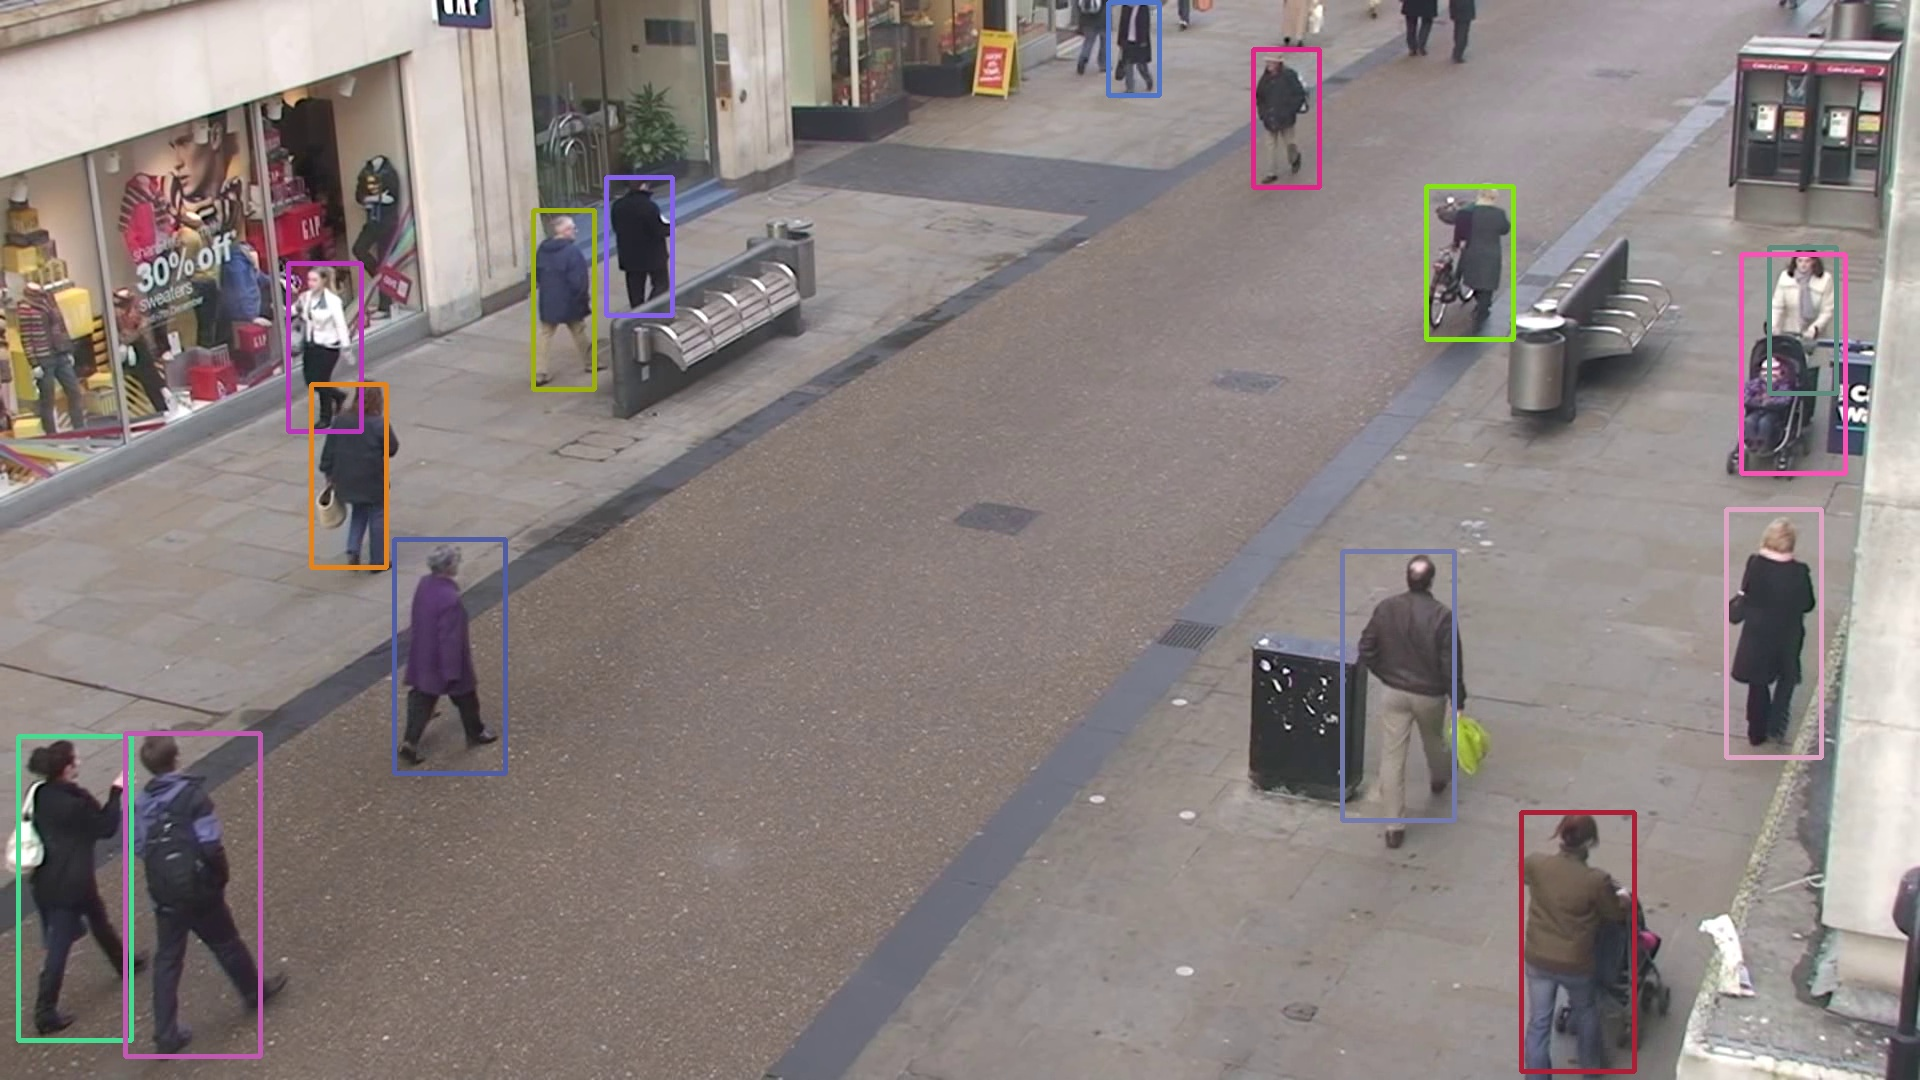
\includegraphics[width=4.6cm]{intro/deteccions.jpg}}
\subfigure[Features Points.]{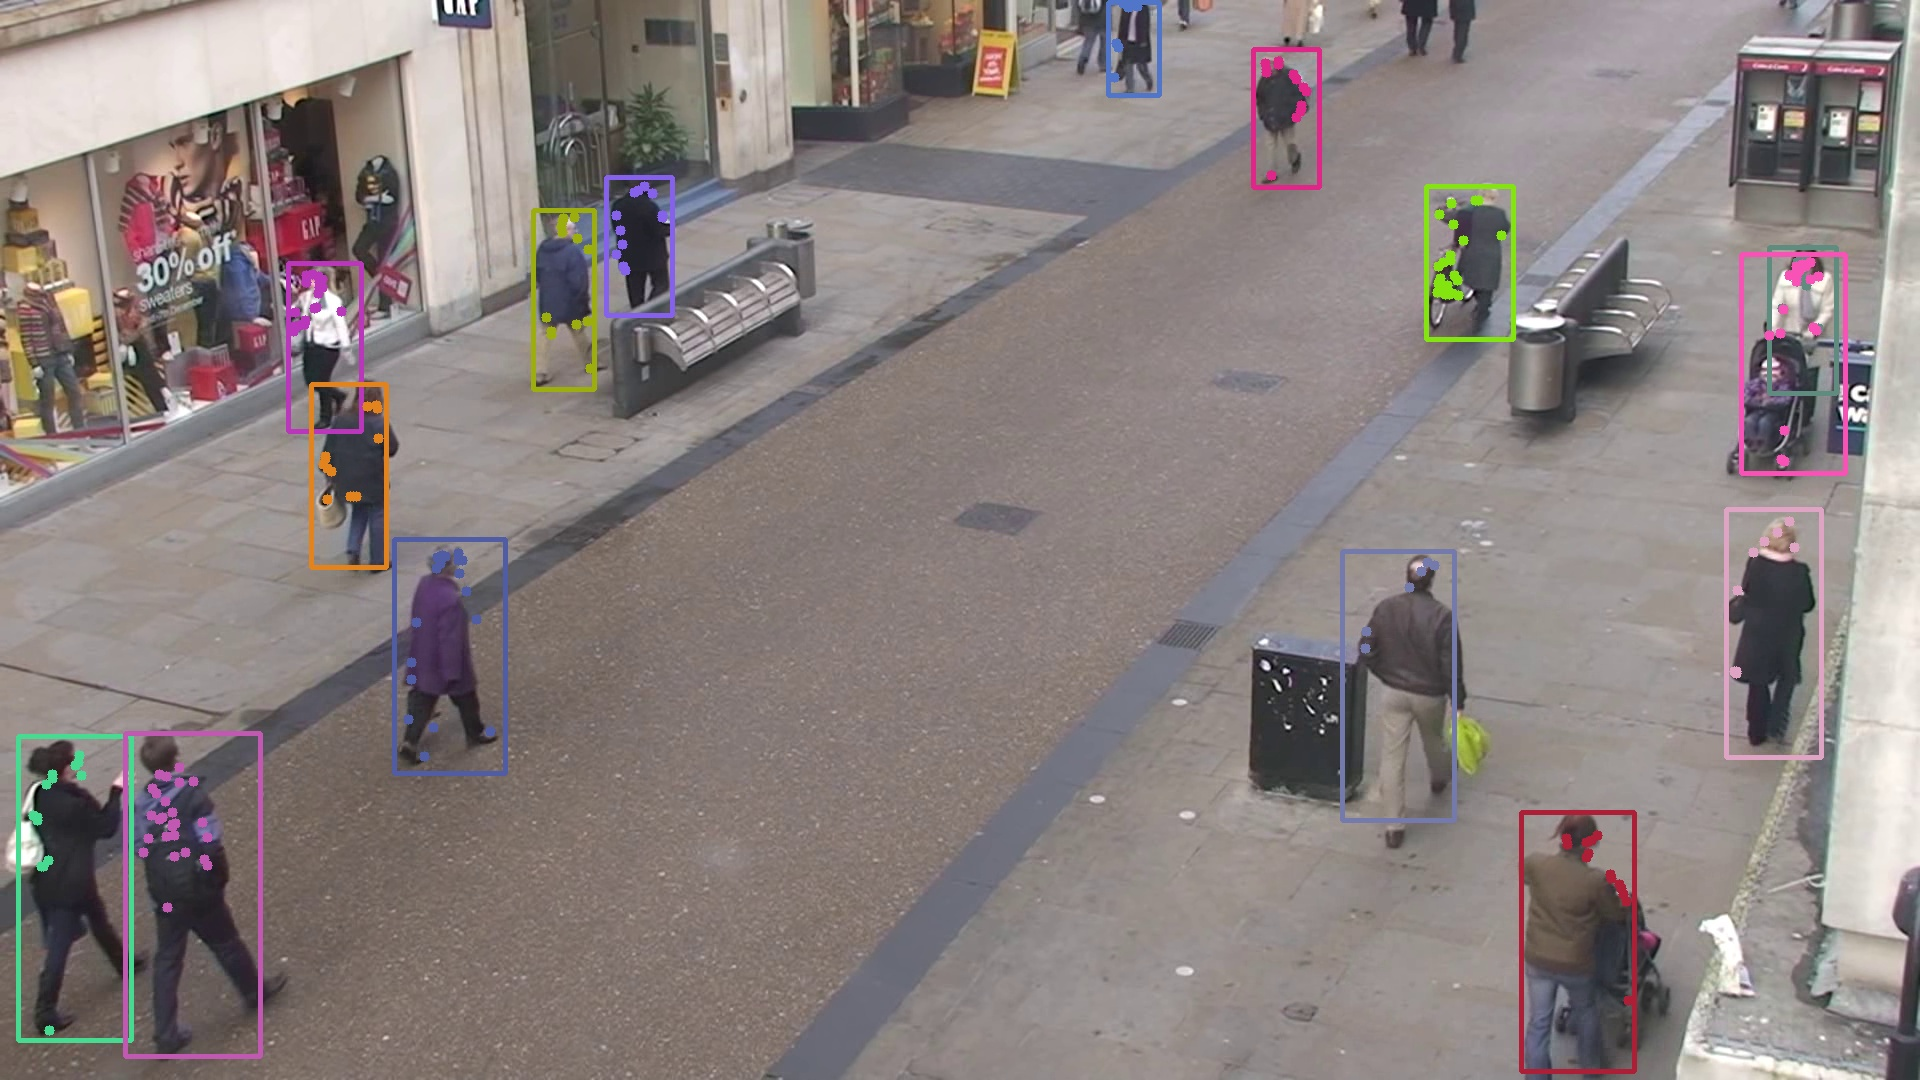
\includegraphics[width=4.6cm]{intro/pounts.jpg}}
\subfigure[Optical flow.]{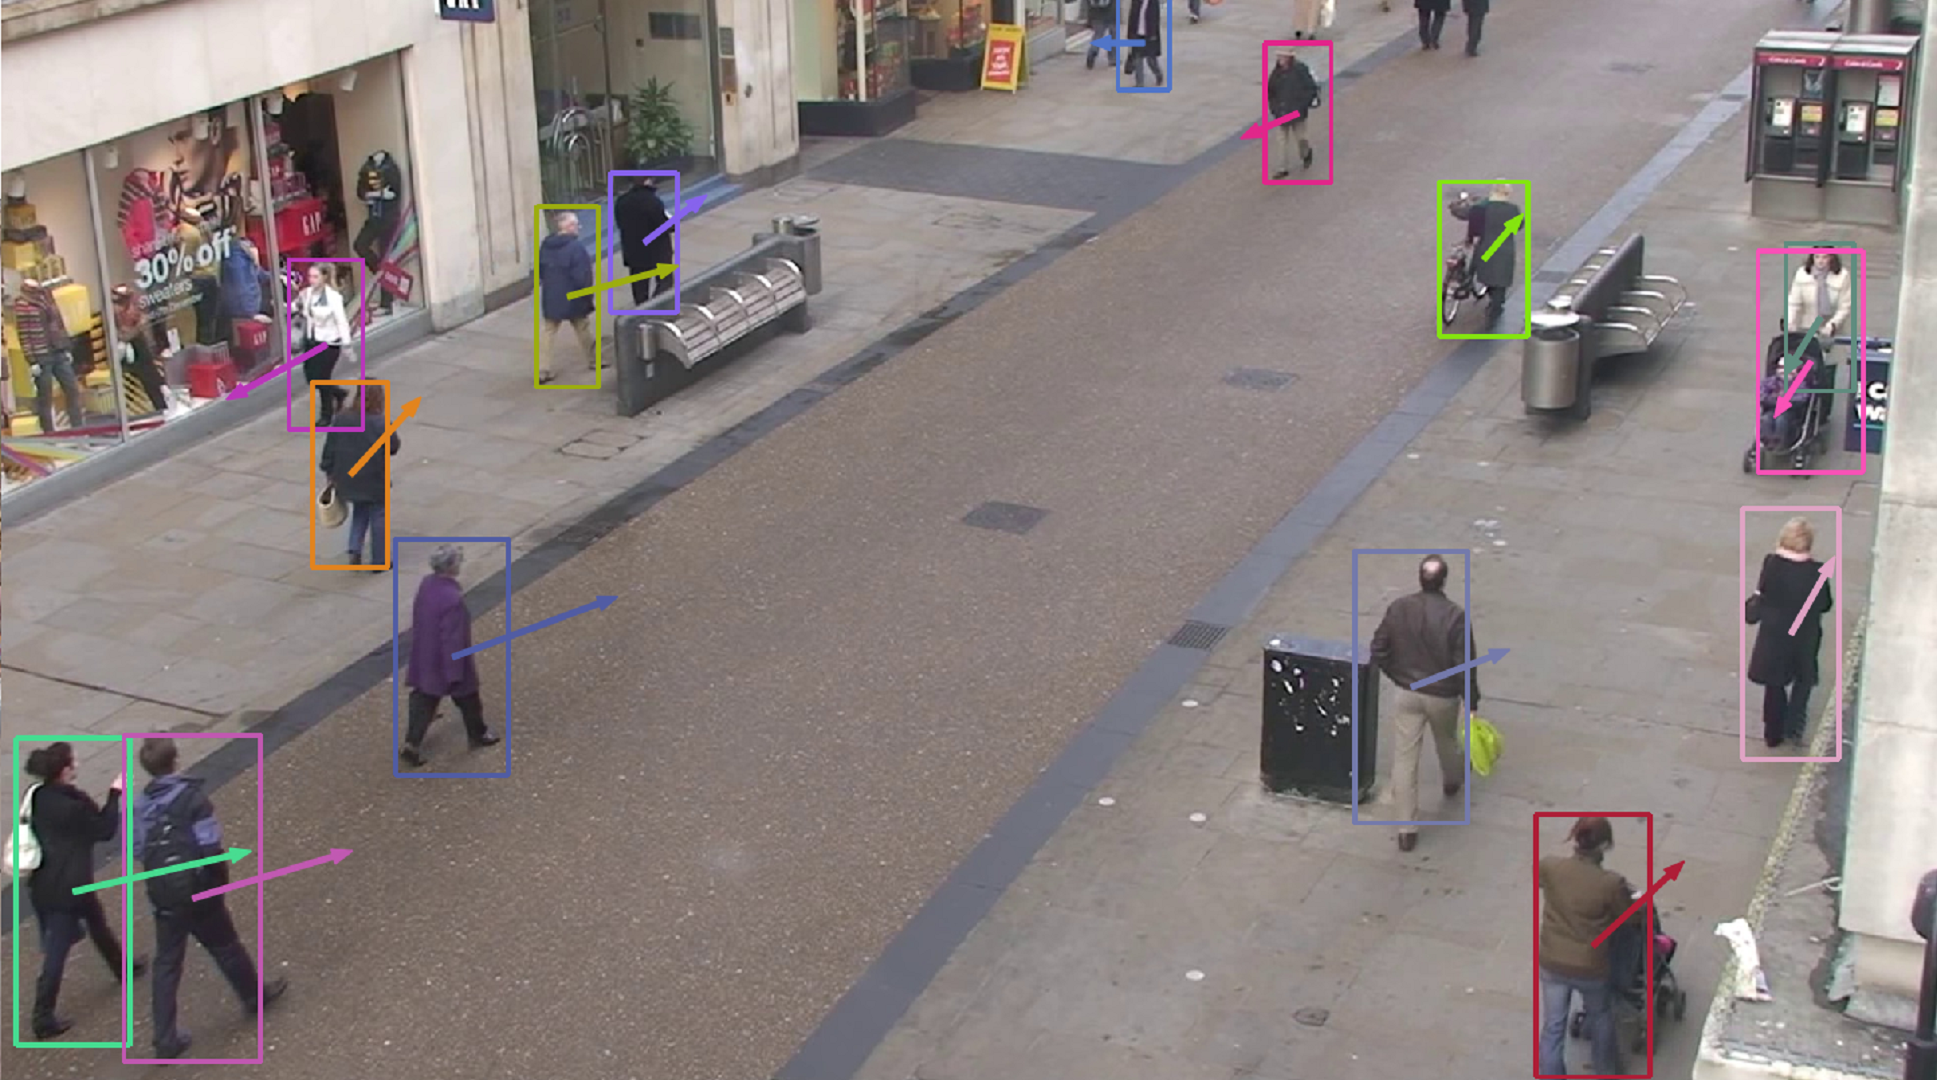
\includegraphics[width=4.6cm]{intro/alcover2.png}}
\subfigure[Identity check.]{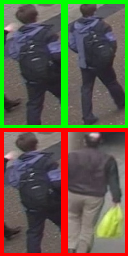
\includegraphics[height=2.6cm]{intro/out2.png}}\\


\caption{Algorithm's stages.}
\label{stepsAlgo}
\end{figure}

\subsection{Object detection}\label{trackingBounding}






In object detection too, the emergence of the neural networks has supposed a turning point. As we can observe in \ref{deepObjet}, the mean average precision, has almost doubled since the appearance of deep neural networks.


\begin{figure}[H]
\centering         
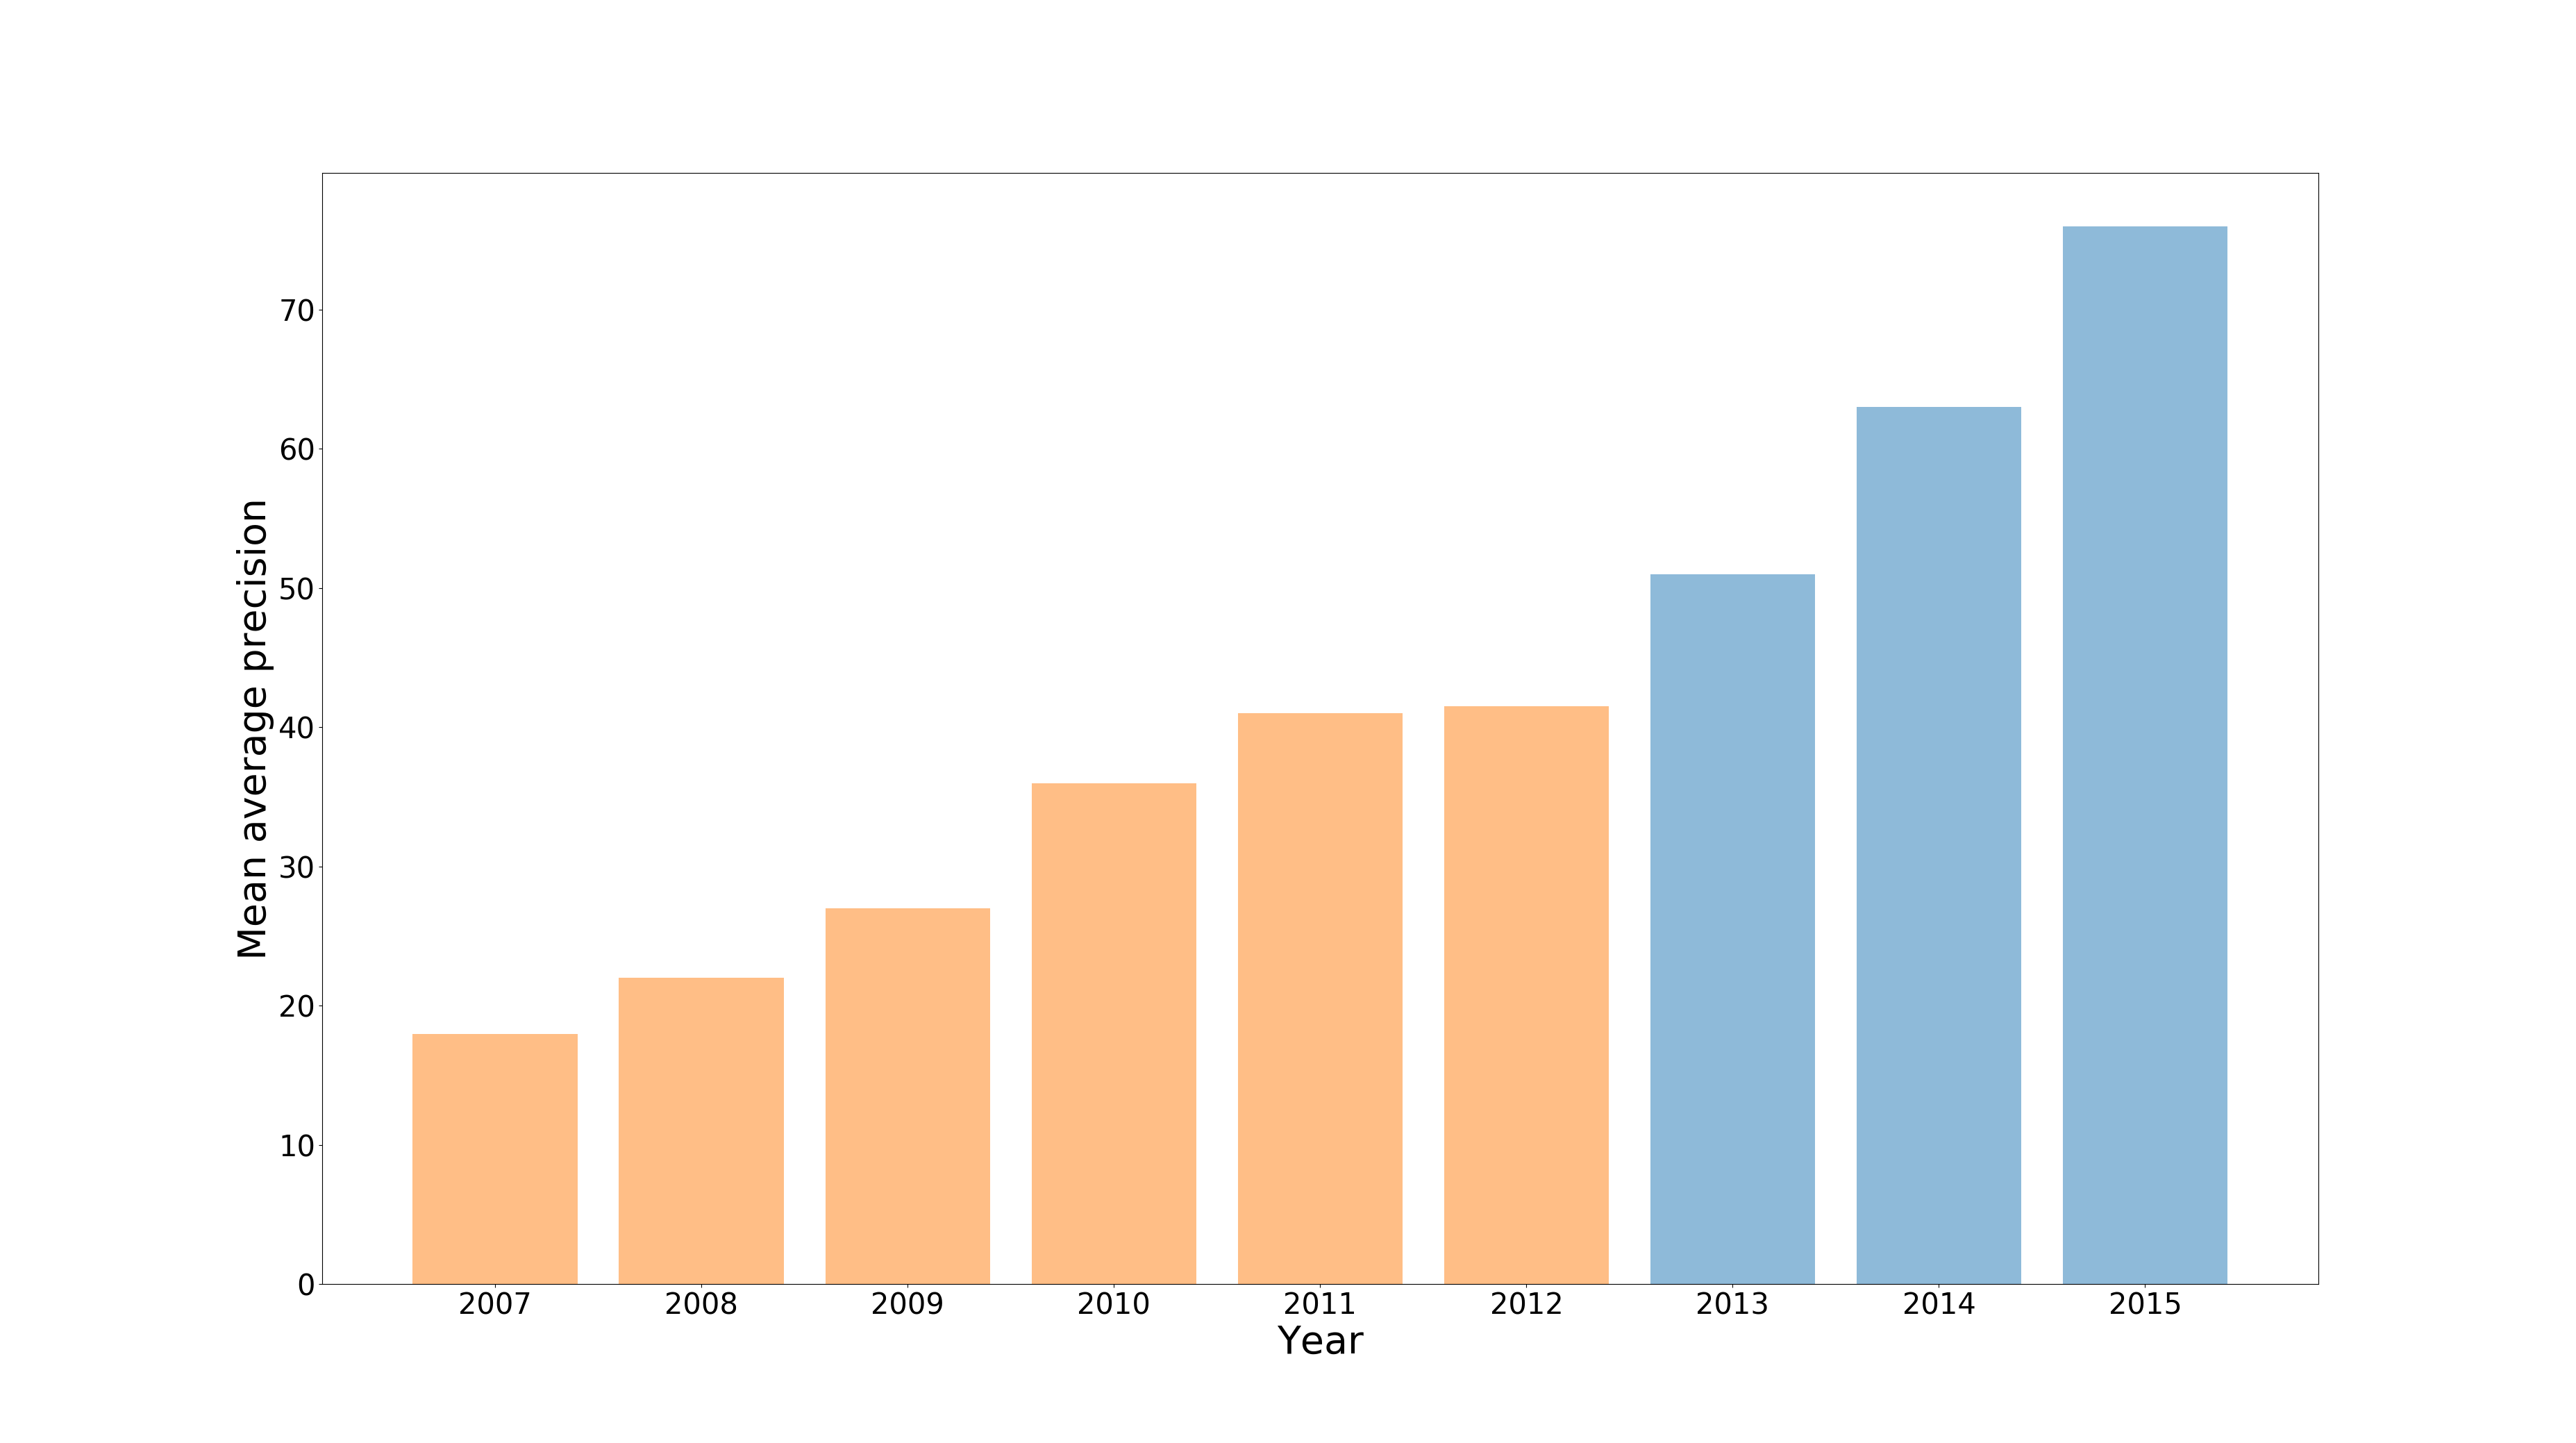
\includegraphics[width=0.7\linewidth]{intro/objesName.png}
\caption{Mean average precion over the years in PASCAL dataset.} \label{deepObjet}
\end{figure}


%Actual object detectors are based on three main family of archictectures \cite{cnnComparision}, of which names are: FasterRCNN, RFCN, and SSD. In \ref{refArchite} we can observe a scheme of these systems.


Present deep learning object detectors are based on three main family of archictectures \cite{cnnComparision}, named by the reference algorithm of the category: FasterRCNN, SSD, and RFCN, the characteristics of these systems are:

%\begin{figure}[H]
%		
%\centering
%
%\subfigure[Faster RCNN.]{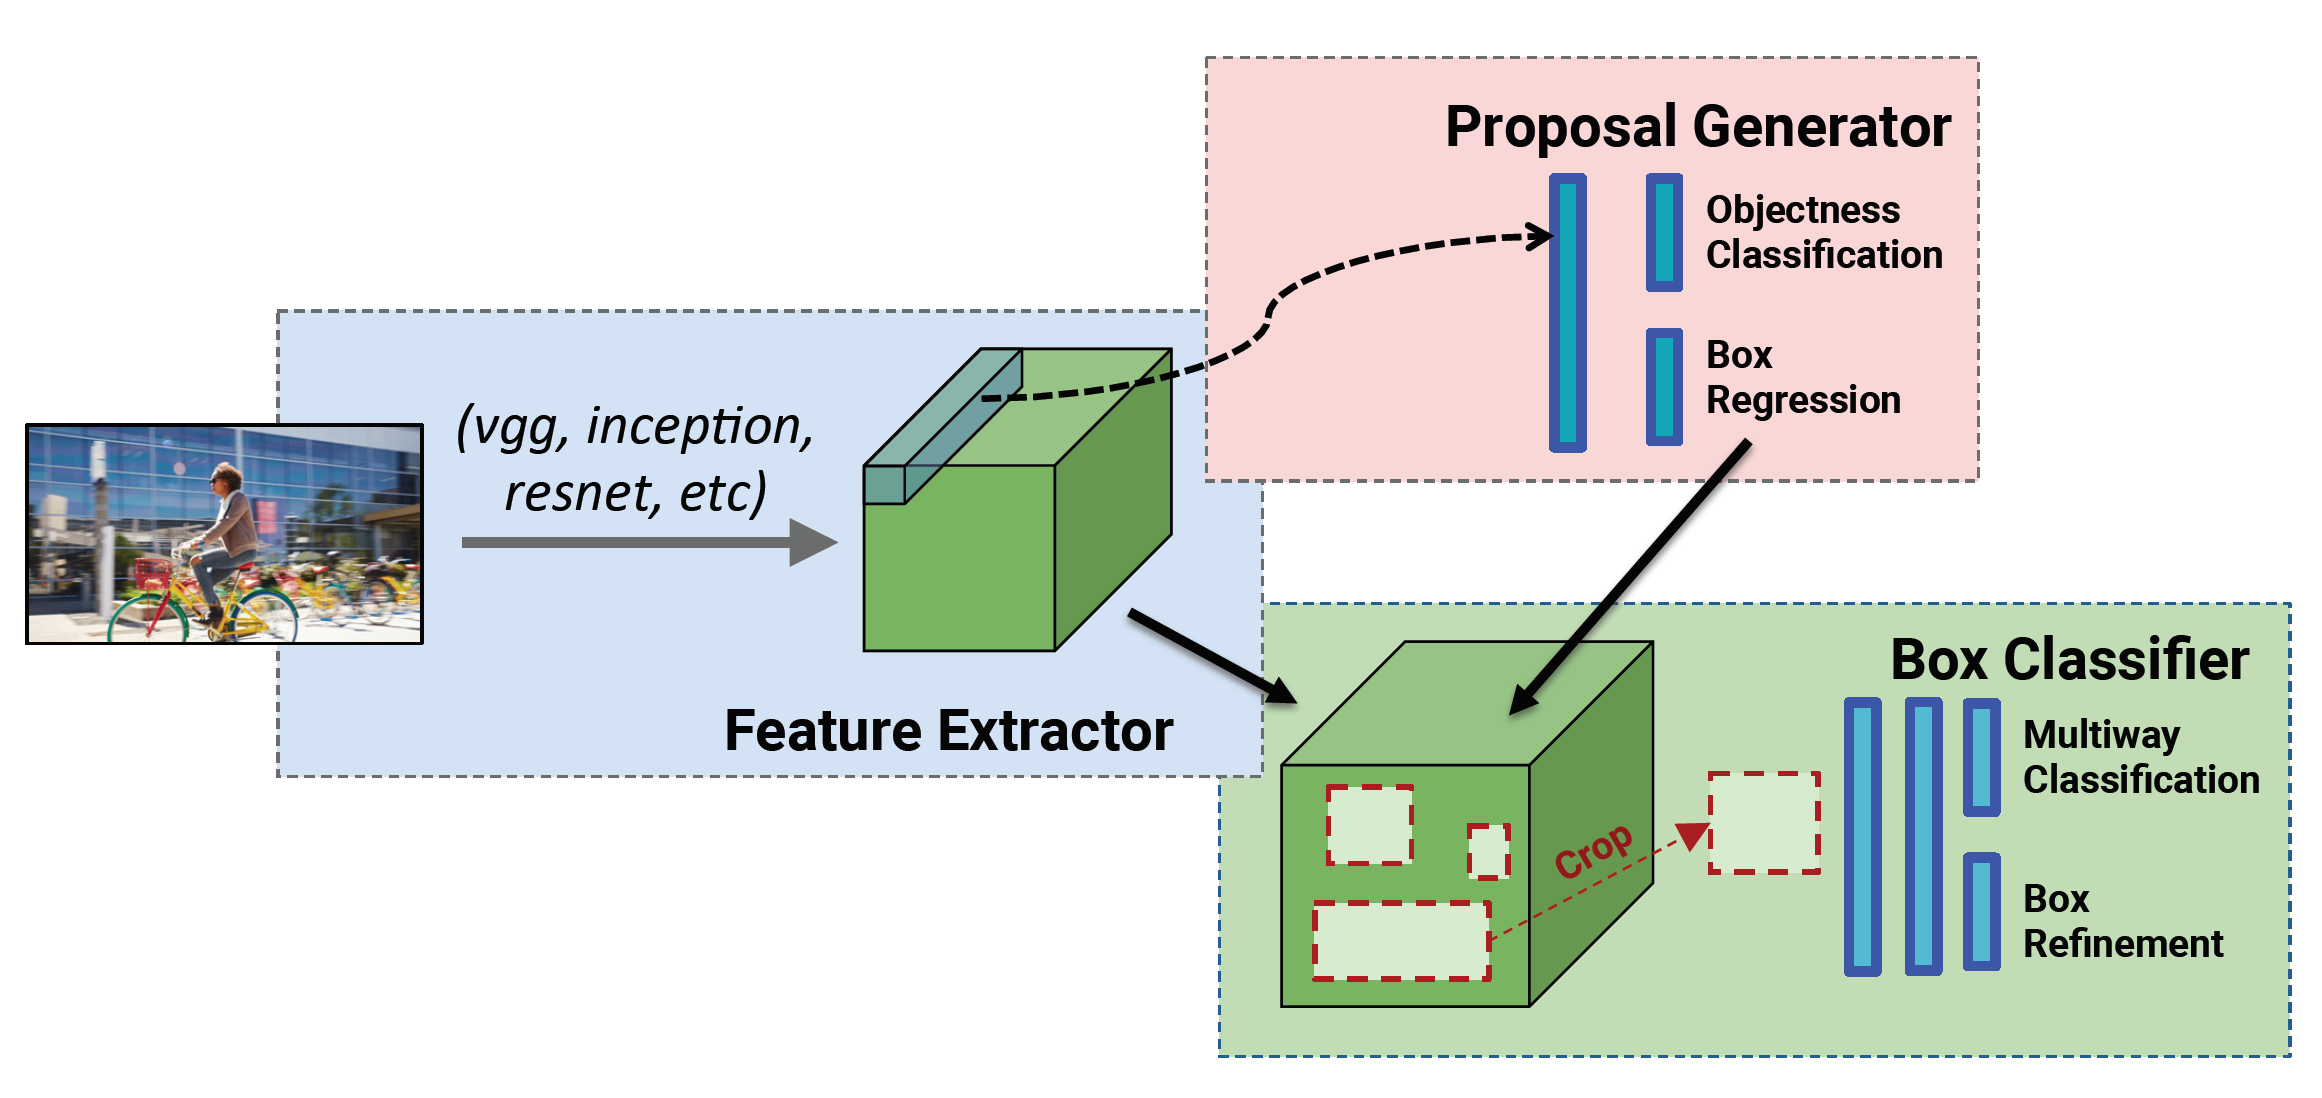
\includegraphics[width=5cm]{objectDetection/compFaster.png}}
%\subfigure[SSD.]{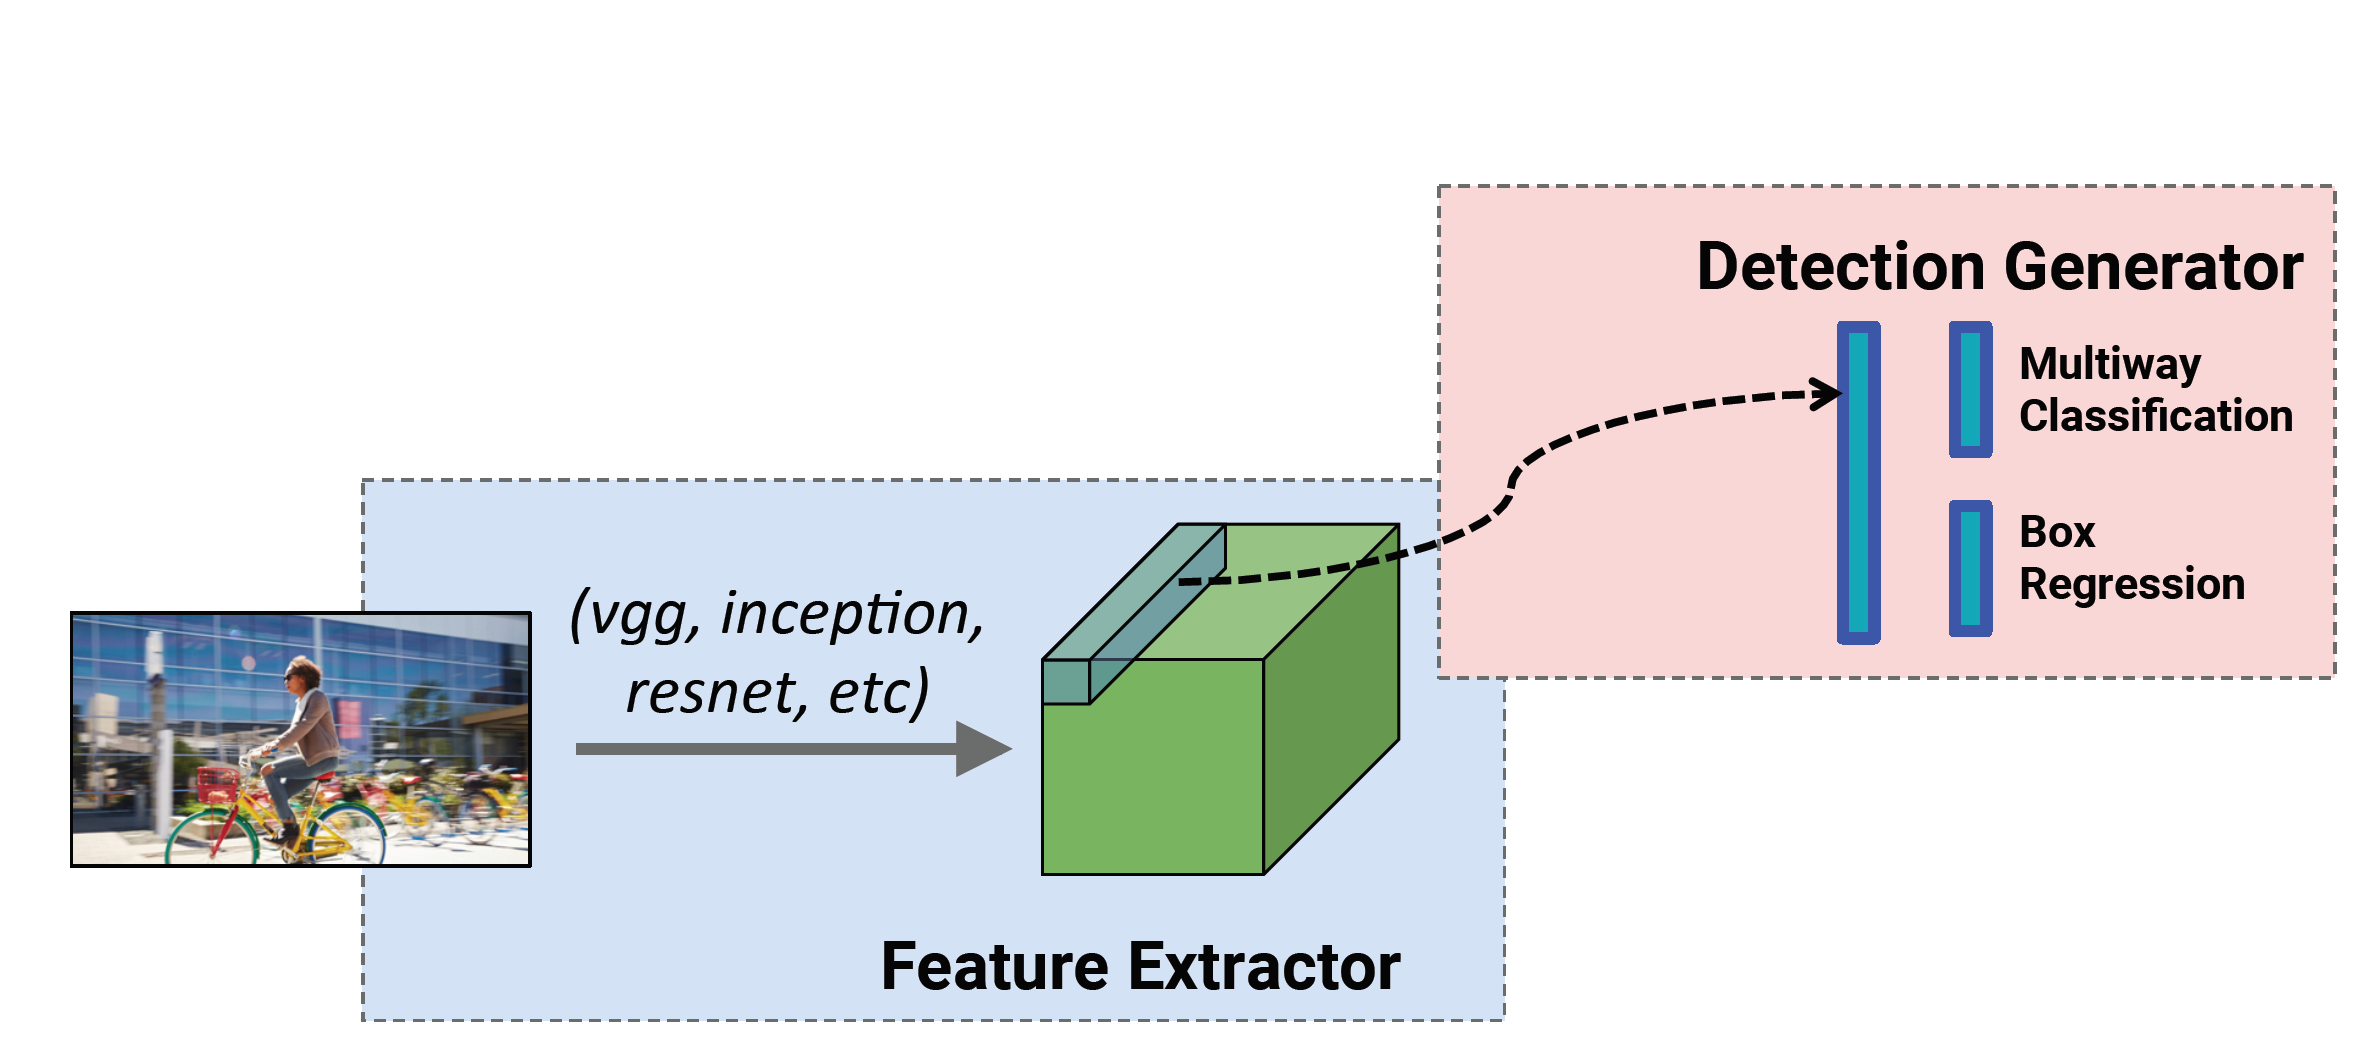
\includegraphics[width=5cm]{objectDetection/compSSD.png}}
%\subfigure[RFCN.]{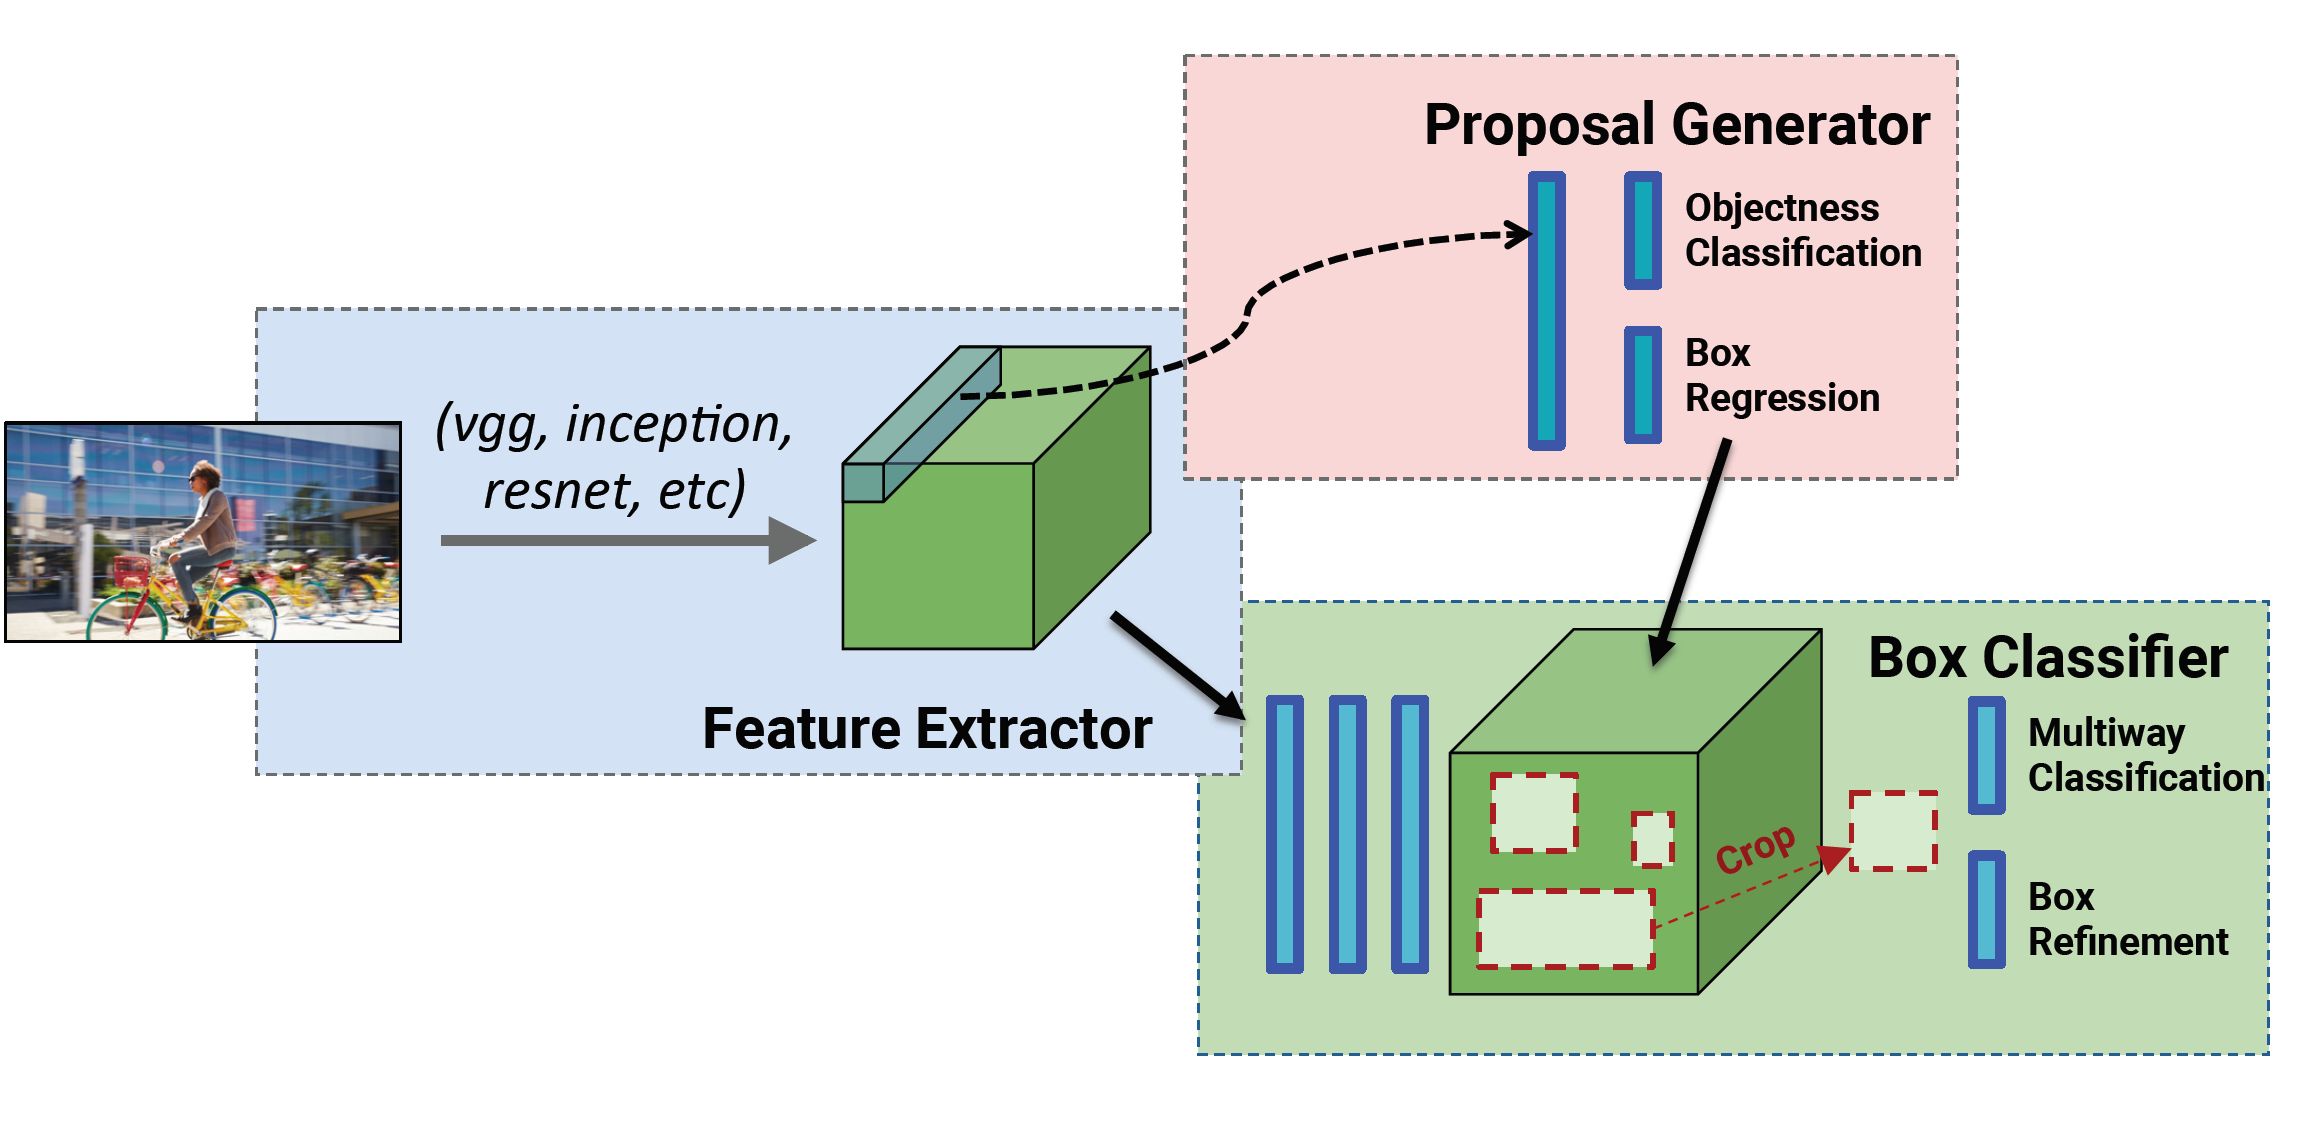
\includegraphics[width=5cm]{objectDetection/compRFCN.png}}\\
%
%\caption{Object detection architectures.}
%\label{refArchite}
%\end{figure}



\begin{itemize}

\item Faster RCNN \cite{fasterrcnn}, it is the last output of a tryology of detectors developed by R. Girshick and his team. Which are called Region-Based object detecors. They work as follows: Use some mechanism to extract region of an image that are probable to be an object and then classify those proposals with a CNN. The first paper to do so, was \cite{rcnn}, and supposse a breaktrough in the field, increasing the precision of the state of the art of those days. But, it had a messy pipeline, slow and difficult to train. Later on, they developed \cite{fastrcnn}, in this paper they applied the region proposal algorithm in the cnn feature map, so, they avoid to compute the features for each proposal. They increase the speed and it could be trained much easily. Finally, they showed FasterRCNN \cite{fasterrcnn}, in this algorithm, they eluded the external region proposal algorithm and they implemented a CNN to compute those proposals. This CNN share parameters with the main net and they saved a lot of time. This network, has become the standard object detector with CNN. With the association of novel net architecture like ResNet \cite{resnet}, Inception \cite{inception}, and \cite{pvanet} they have won all the contests.


\item SSD, it stands fot Single shot multibox detector. These family of method differs from previous ones considering that these treats the problem of object detection as a regression problem. So, they are called Regression-based object detector or single shot object detector due it does not have a region proposal algorithm, they classify the image with one mechanism. The maximium exponent of these algoirthms are \cite{yolo} and \cite{ssd}. These work as follows, they discretize the image at the features level in a fixed grid and for each grid it predicts a class and some number of bounding boxes with different shapes and sizes. It merges all, and apply a Non-Maximum supression algorithm to obtain a set of detections. We can observe this process in \ref{yolo1}. In addition, they apply this process in a multiresolution scheme as we can observe in \ref{yolo2} to deal with objects of different sizes.

%\item RFCN \cite{rfcn}, it stands for Region-based fully convolutional network and it was developed by the same authors of SSD. It is based on a Region-based architecture, altough after the feature map they add an region-sensitive layer, this layer activates in the position where there are an object. It has an inspiration in the architectures fully convolutional used in semantic segmantic.

\begin{figure}[H]
		
\centering

\subfigure[Input Image.]{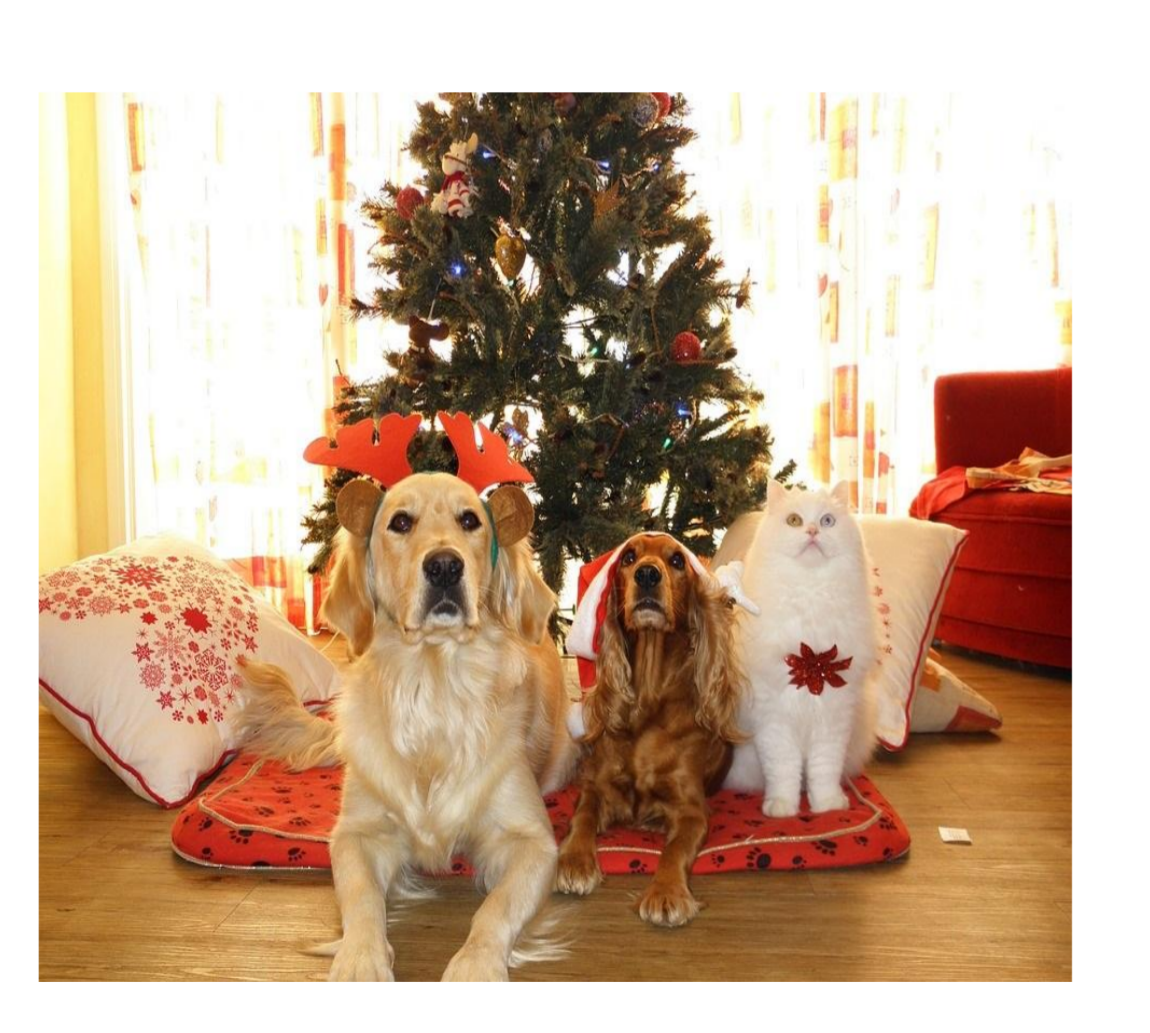
\includegraphics[width=7cm]{objectDetection/retall1.png}}
\subfigure[Divide image into grid.]{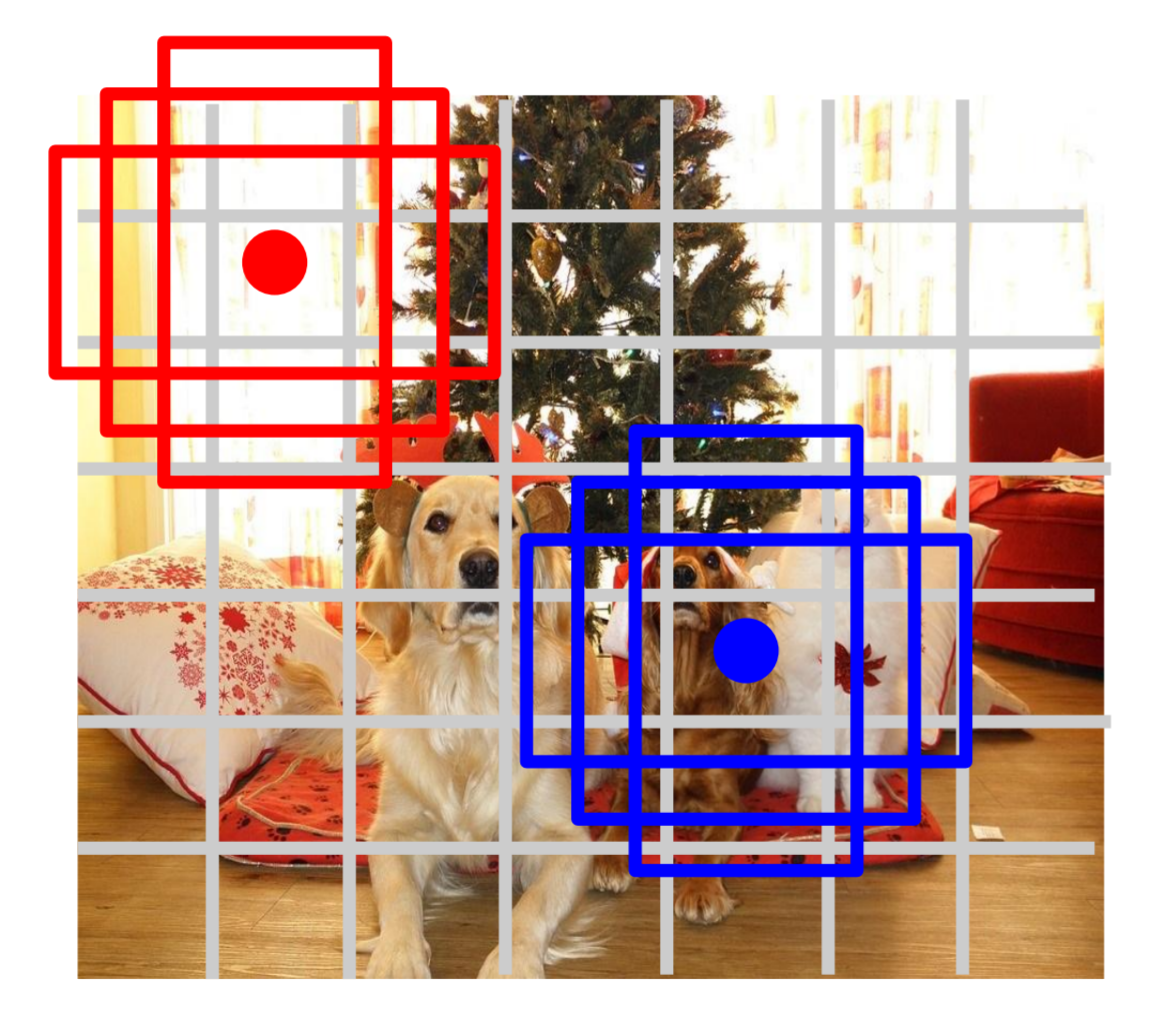
\includegraphics[width=7cm]{objectDetection/retall2.png}}\\


\caption{SSD detector scheme.}
\label{yolo1}
\end{figure}


\begin{figure}[H]
\centering         
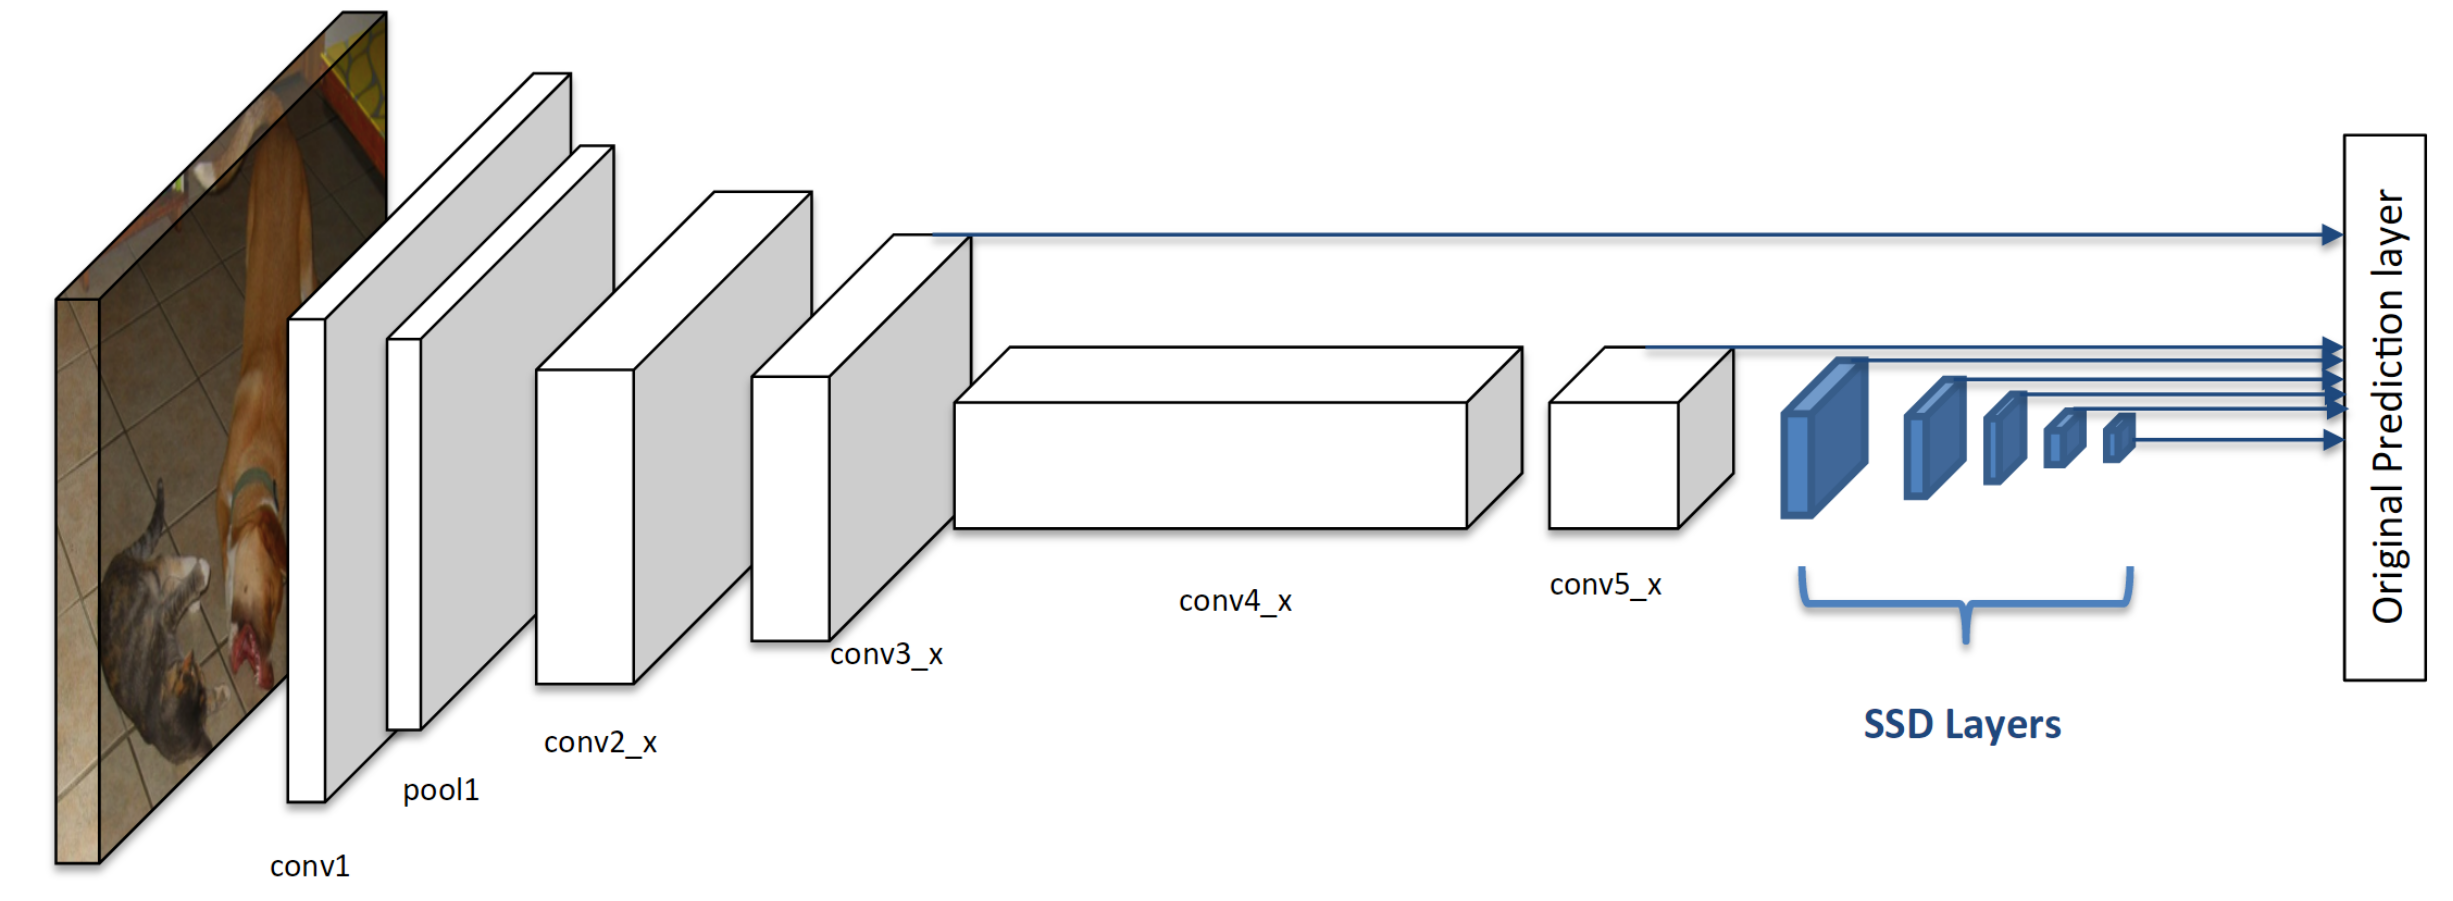
\includegraphics[width=12cm]{objectDetection/ssdArchitecture2.png}
\caption{SSD architecture.} \label{yolo2}
\end{figure}



\item RFCN \cite{rfcn}, it stands for Region-based fully convolutional network and it was developed by the same authors of SSD. They noticed the lacks of the SSD, the SSD algorithm computes the object detector on the feature map, and at this level the features have a low spatial resolution, this involves do not detect small objects. So the authors inspired by the fully convolutional architectures, upsample those feature maps and compute the object detector like the SSD algorithm.

\end{itemize}



%\begin{figure}[H]
%		
%\centering
%
%\subfigure[Input Image.]{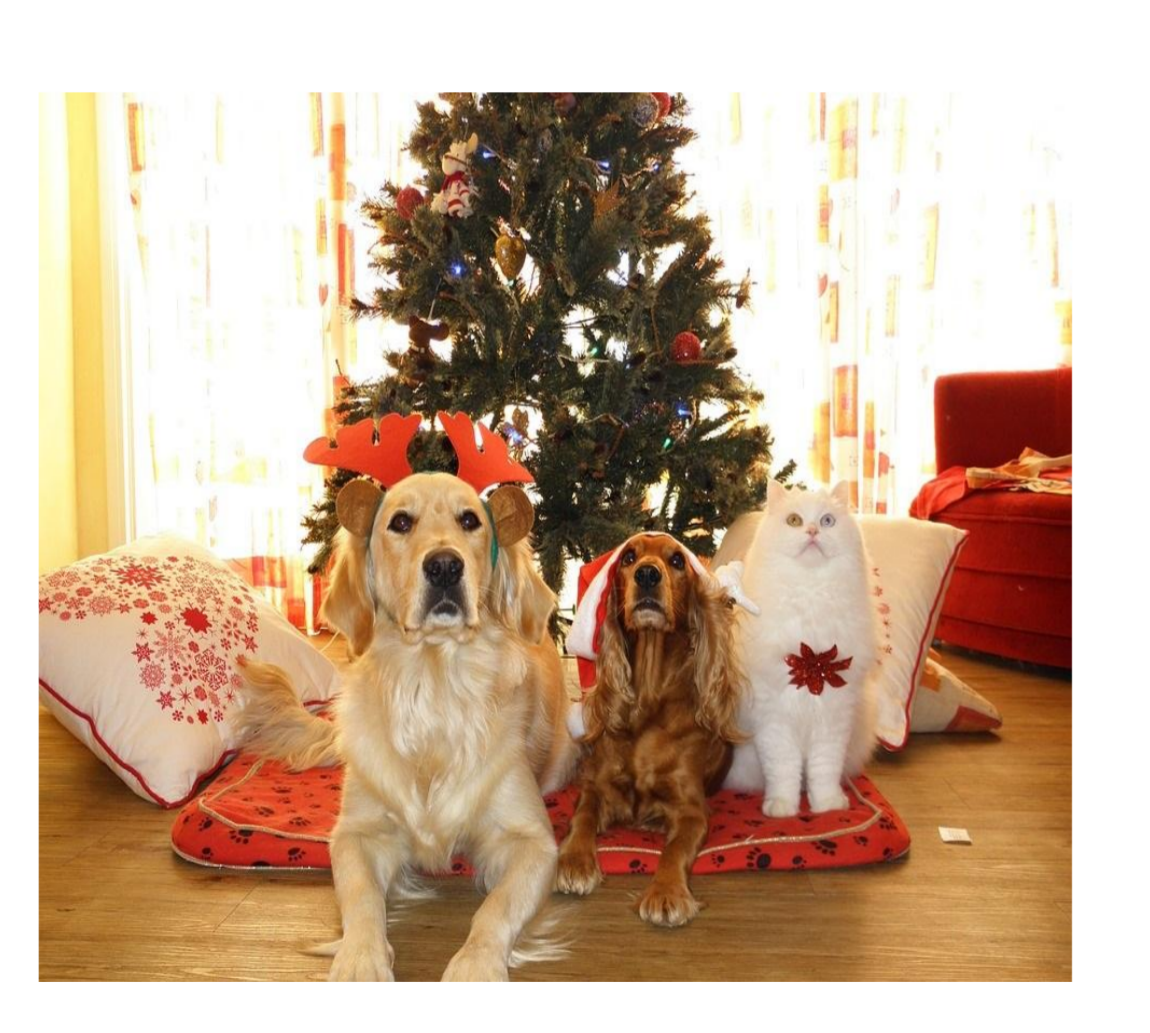
\includegraphics[width=7cm]{objectDetection/retall1.png}}
%\subfigure[Divide image into grid.]{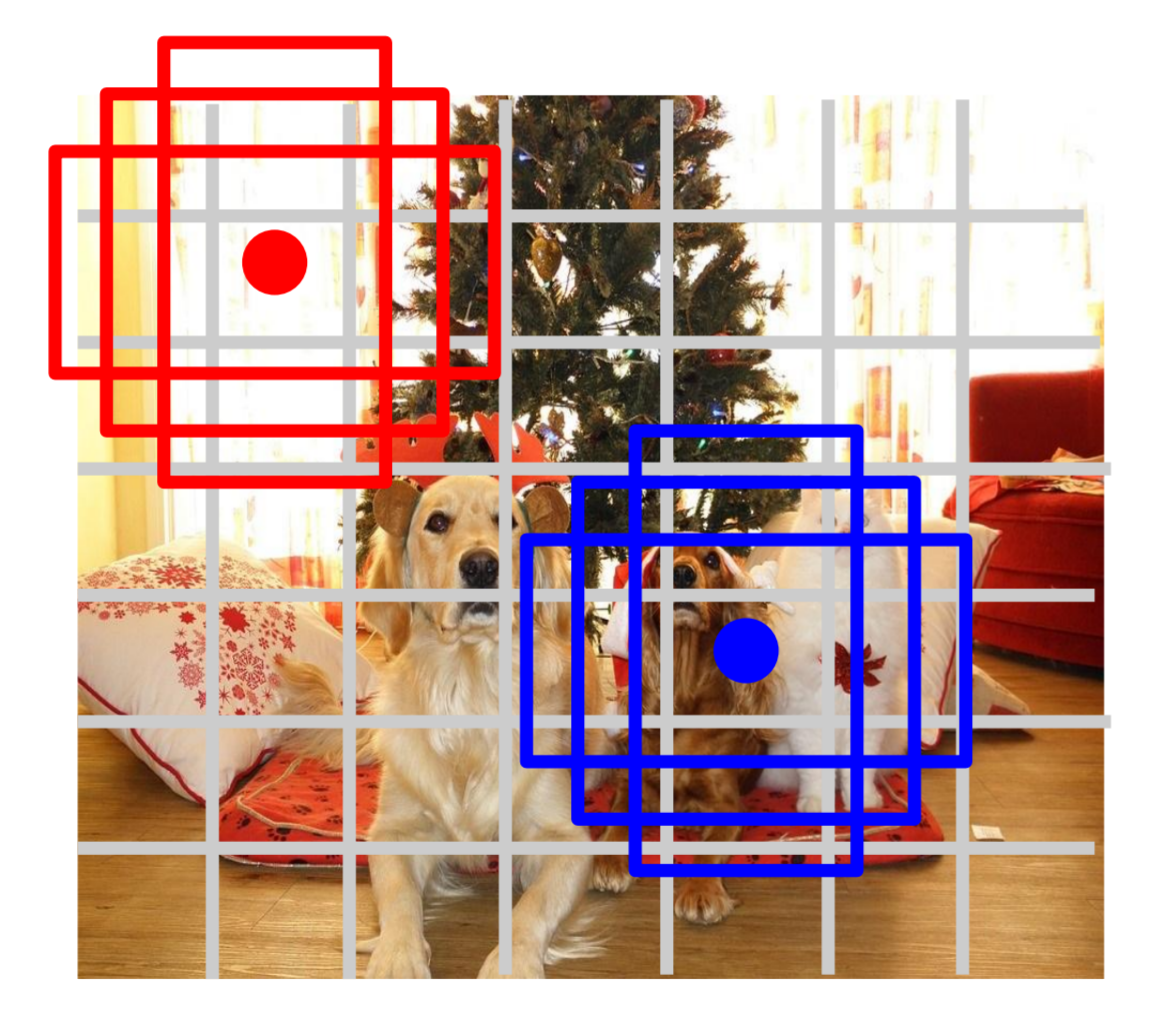
\includegraphics[width=7cm]{objectDetection/retall2.png}}\\
%
%
%\caption{SSD detector scheme.}
%\label{yolo1}
%\end{figure}
%


%\begin{figure}[H]
%\centering         
%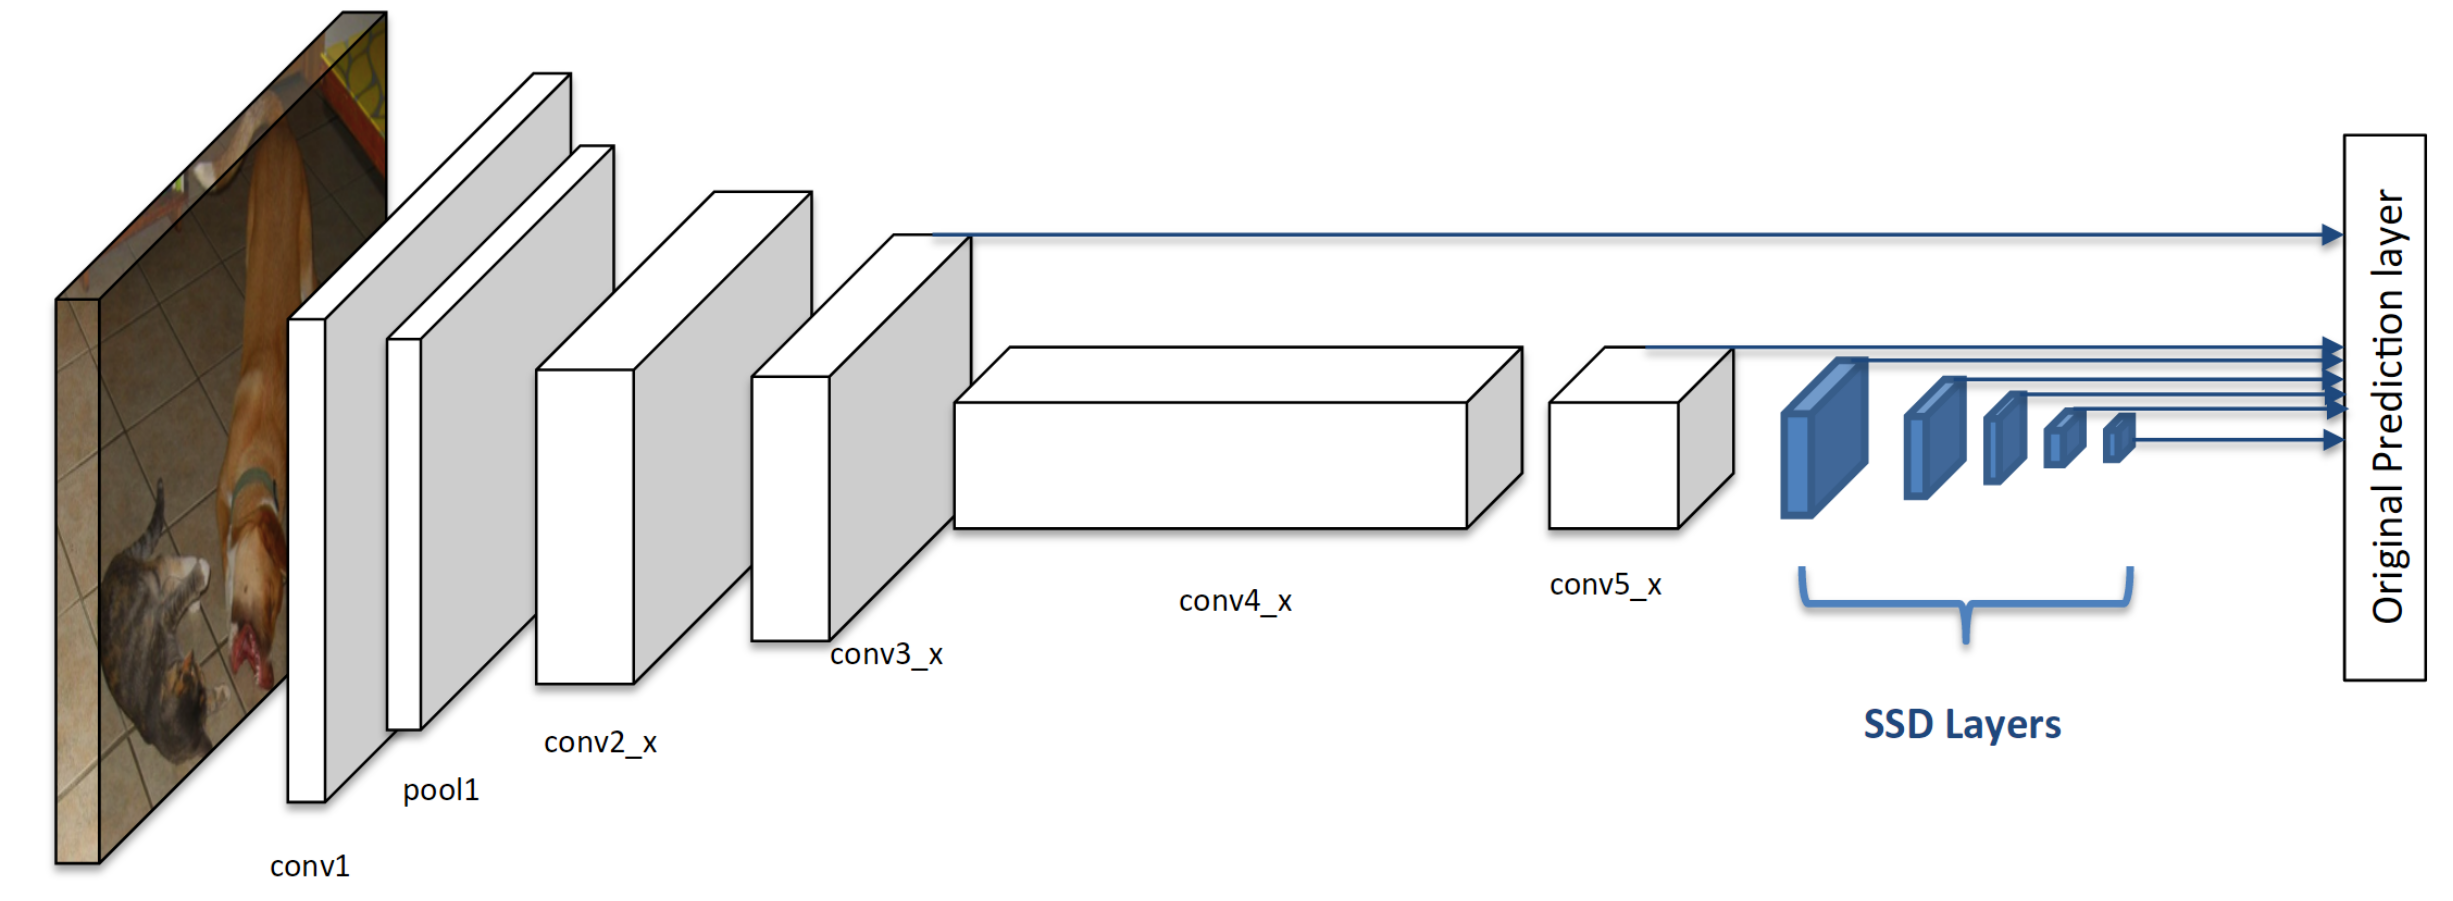
\includegraphics[width=12cm]{objectDetection/ssdArchitecture2.png}
%\caption{SSD architecture.} \label{yolo2}
%\end{figure}


In the survey \cite{cnnComparision}, they compared the different methods including changing the features extractors ( ResNet, Inception, VGG ) and they measured the precision ( mean average precision ) and computing time. This results are showed in \ref{comparisio}. The conlcusion are as follows, SSD is the fastest detector, RFCN it has the best balance between speed-acurracy, and FasterRCNN, is the most acurate detector altough is slower than the other ones.



\begin{figure}[H]
\centering         
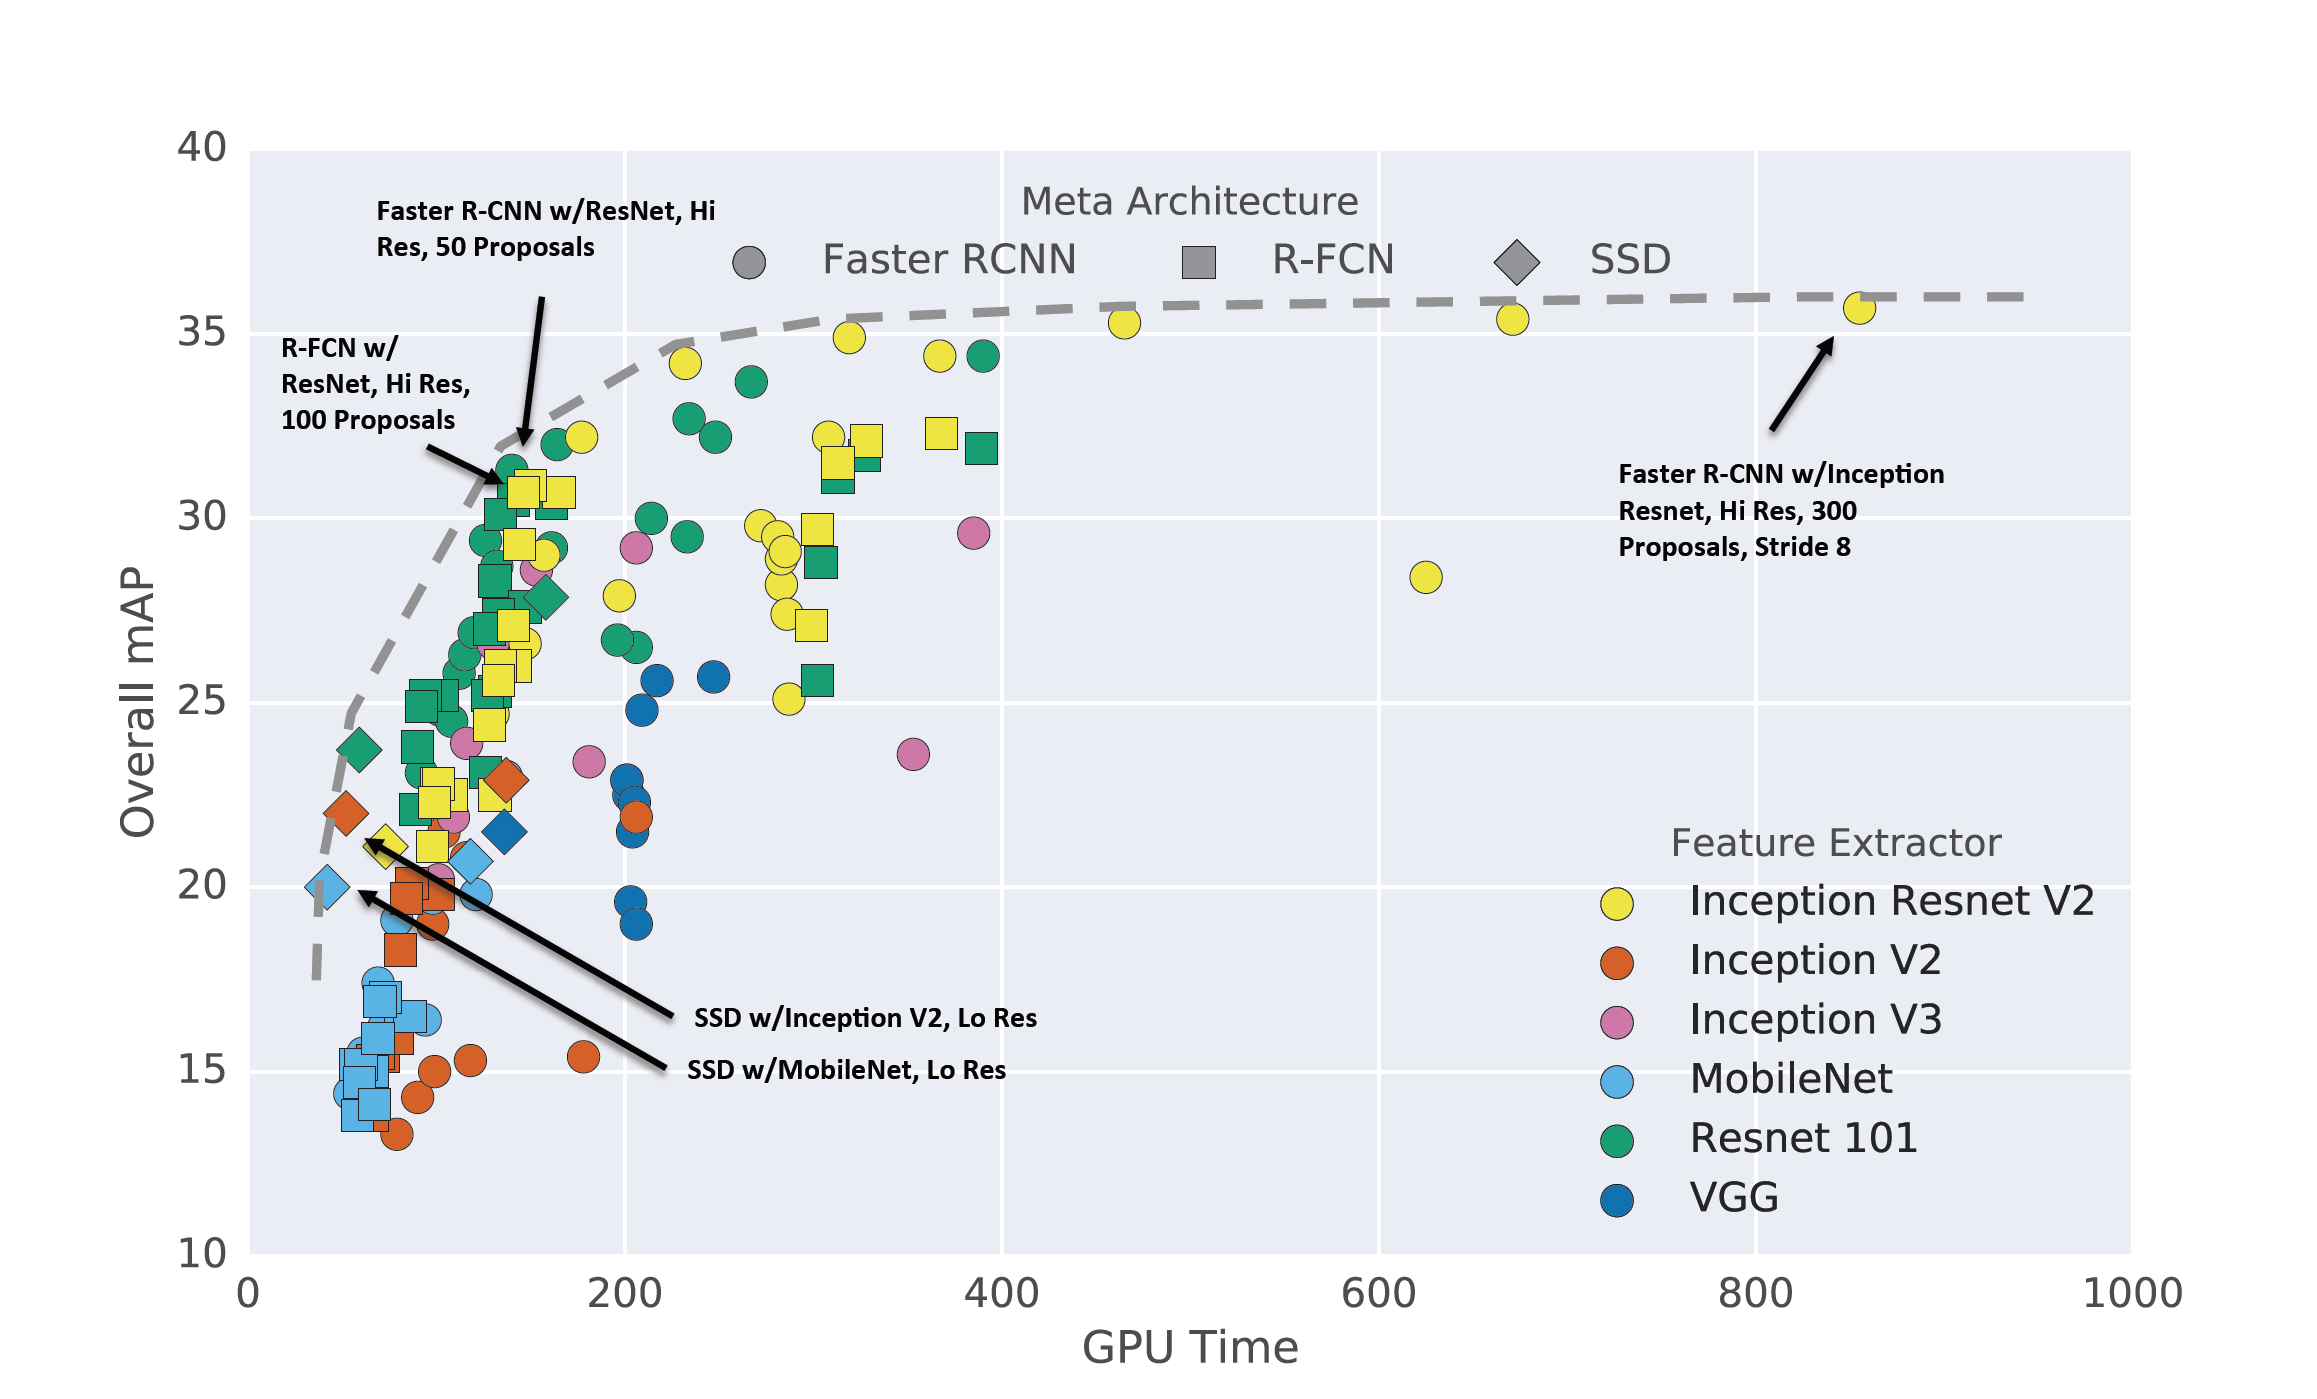
\includegraphics[width=0.9\linewidth]{objectDetection/comparisionTensor.png}
\caption{Comparision architectures.} \label{comparisio}
\end{figure}

We will finish off our review with a numeric comparision of the methods, as we can observe in the table \ref{tableDet}. This information is extracted from the original papers with their implementation, all of them are trained with the union of the training set of VOC07, VOC12, and COCO, and subsequently evaluate on VOC07 test set on a Nvidia Titan X GPU.   

\begin{table}[H]
\centering

\begin{tabular}{lllll}
                    & \textbf{mAP} & \textbf{mAP\_person} & \textbf{FPS} & \textbf{Proposals} \\
\textit{RCNN}       & 66           & 64.2                 & 0.077        & 2000               \\
\textit{FastRCNN}   & 70           & 69.9                 & 6.7          & 2000               \\
\textit{FasterRCNN} & 85.6         & 82.3                 & 7            & 6000               \\
\textit{SSD300}     & 81.2         & 81.4                 & 46           & 8732               \\
\textit{SSD512}     & 83.2         & 84.6                 & 19           & 24564              \\
\textit{YOLO}       & 66.4         & 63.5                 & 45           & 98                 \\
\textit{YOLOv2}     & 78.6         & 81.3                 & 40           & -                  \\
\textit{RFCN}       & 83.6         & -                    & 10           & -                  \\
\textit{PVANET}     & 84.9         & -                    & 31.3         & 300               
\end{tabular}

\caption{Summarize of the object detectors.}
\label{tableDet}
\end{table}







\subsection{Tracking fundamentals}\label{trackingIssues}

As we said above, we need to find features in the image and study how they move to estimate the movement of the targets.

\subsubsection{Features}\label{feature}

Our goal is to find points in an image, that can be found in other images and then compute some information, in this case, the movement. The characteristics of good features are:

\begin{itemize}

\item Repeatability, the same feature can be found in several images despite geometric and photometric transformations.

\item Matchability, each feature has a distinctive description, thus easy to find.

\item Efficiency, few features have to compact much more possible information.

\item Locality, a feature occupies a relatively small area of the image, so therefore it is robust to clutter and occlusion.

\item Perfomance, computation speed of features is a critical parameter. 

\end{itemize}

Features points are used in all sort of operations in computer vision: Image alignment, 3D reonstruction, Motion Tracking, Object recognition, Index database retrieval, robot navigation and so on.

%How can we find image locations where we can reliably find correspondes with other images.

Looking at the figure \ref{patches}, the flat patch, is a patch without texture and impossible to localize. Patches with large contrast edges are easier to localize, although straight lines segments at a single orientation suffer from the \textit{aperture problem}, are also impossible to localize. Finally, patches with large gradients in at least two different orientations are the easiest to localize.

\begin{figure}[H]
		
\centering

\subfigure[Flat region.]{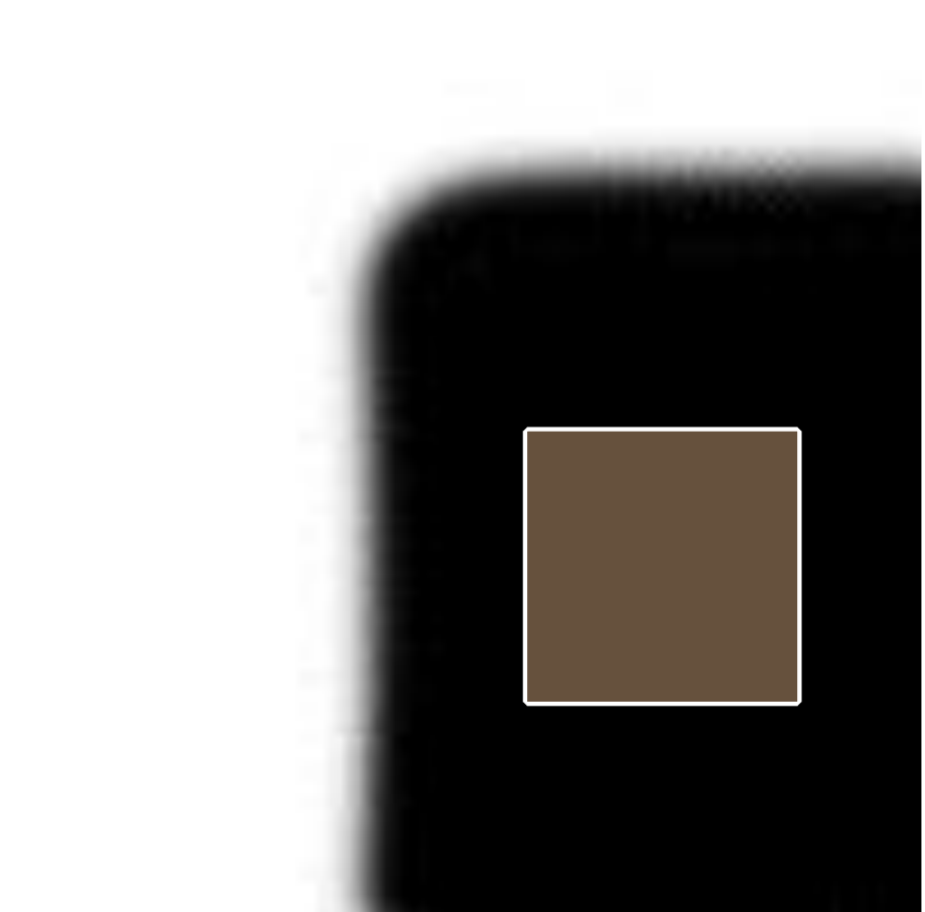
\includegraphics[width=5cm]{lucasKanade/flat.png}}
\subfigure[Edge region.]{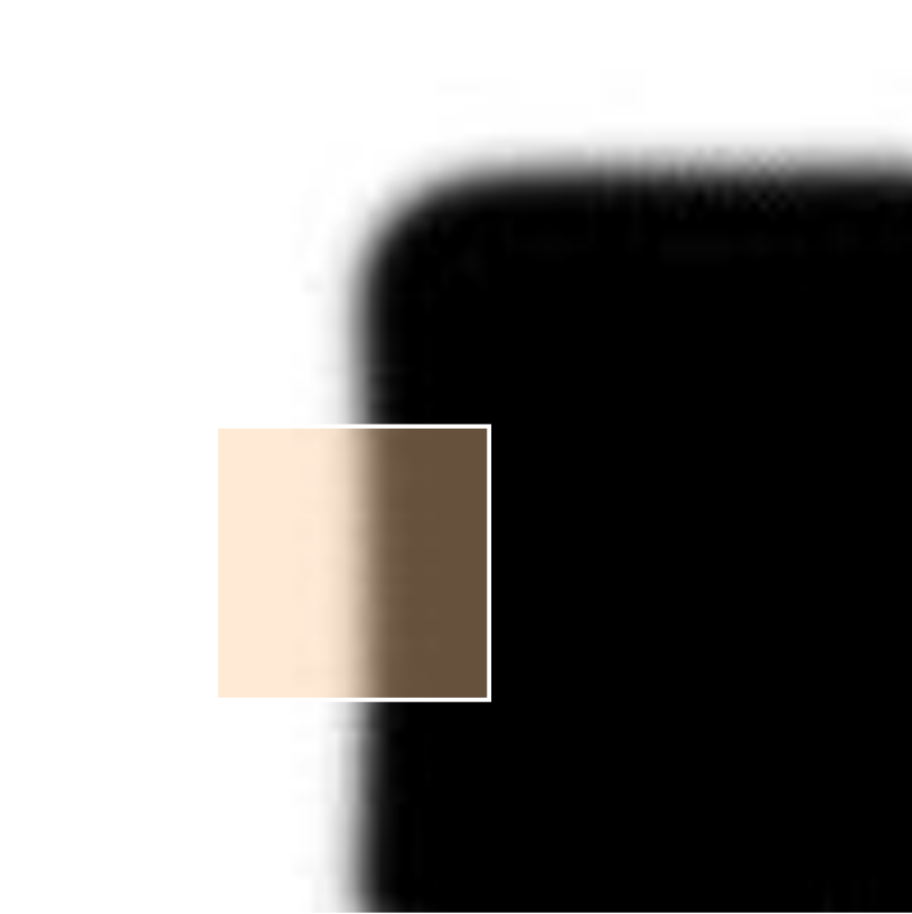
\includegraphics[width=5cm]{lucasKanade/edge.png}}
\subfigure[Corner region.]{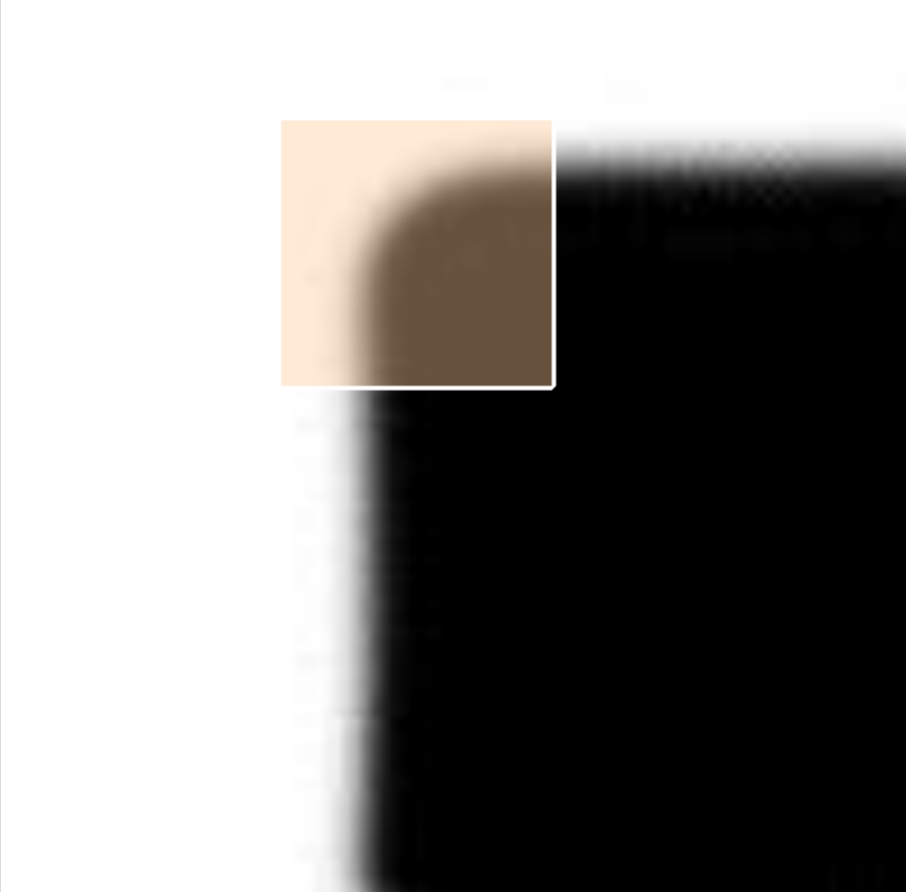
\includegraphics[width=5cm]{lucasKanade/corner.png}}\\


\caption{Types of patches.}
\label{patches}
\end{figure}

These intuitions can be formalized by looking at the simples possible matching criteron for comparing two images patches, their weighted summed square difference:

%Change in appearance for the shift [u,v]:

%$$ E(u,v) = \sum_{x,y} w(x,y) [I(x+u,y+v)-I(x,y)]^{2}$$
$$ E(u) = \sum_{i} w(x_{i}) [I(x_{i}+u)-I(x_{i})]^{2}$$

where $I(x)$ is the image, $I(x+u)$ is the shifted image, and $w(x,y)$ is a window function like a box or gaussian kernal around the pixel, and the summation $i$ is over all the pixels in the patch. Then we are looking for points, which if we move according to $u$ we have a change. 

%In figure \ref{refMovementHarris} we can observe the error $E(u)$ of different positions of the $w(x)$, we can observe that the patch without displacement it does not have an error but if we move it the similarity decresases adn therefore the error increases.

When performing feature detection, we do not know which other image locations the feature will end up being matched against. Therefore, we can only compute how stable this metric is with respect to small variations in positions $\Delta u$ by comparing an image patch against itself:

$$ E( \Delta u) = \sum_{i} w(x_{i}) [I(x_{i}+\Delta u)-I(x_{i})]^{2}$$

Using a Taylor series expansion of the image function $I(x_{i}+\Delta u) \approx I(x_{i}) + \nabla I(x_{i})*\Delta u  $ we can approximate the expresion as follows:

$$ E( \Delta u) \approx \sum_{i} w(x_{i}) [I(x_{i})+\nabla I(x_{i}) \Delta u-I(x_{i})]^{2}$$


$$ E( \Delta u) = \sum_{i} w(x_{i}) [\nabla I(x_{i}) \Delta u]^{2}$$

With algebraic notation it transforms to:

$$ E( \Delta u) = \Delta u^{T} M \Delta u$$

where $ \nabla I(x_{i}) = [I_{x},I_{y}](x_{i}) $ is the image gradient and $M$ is the second moment matrix:

\[ M = \left( \begin{array}{ccc}
I_{x}^{2} & I_{xy}^{2} \\
I_{xy}^{2} & I_{y}^{2} \end{array} \right).\] 

Computing the eigenvalue descompostion of this matrix, shows the directions of the fastest change, thus a measure of the \textit{cornernes}. There are several algorithms that use in different ways this eigenvalues:

%In the figure \ref{corner} we can observe the relationship between eigenvalues and patches types.
%
%
%
%
%\begin{figure}[H]
%\centering         
%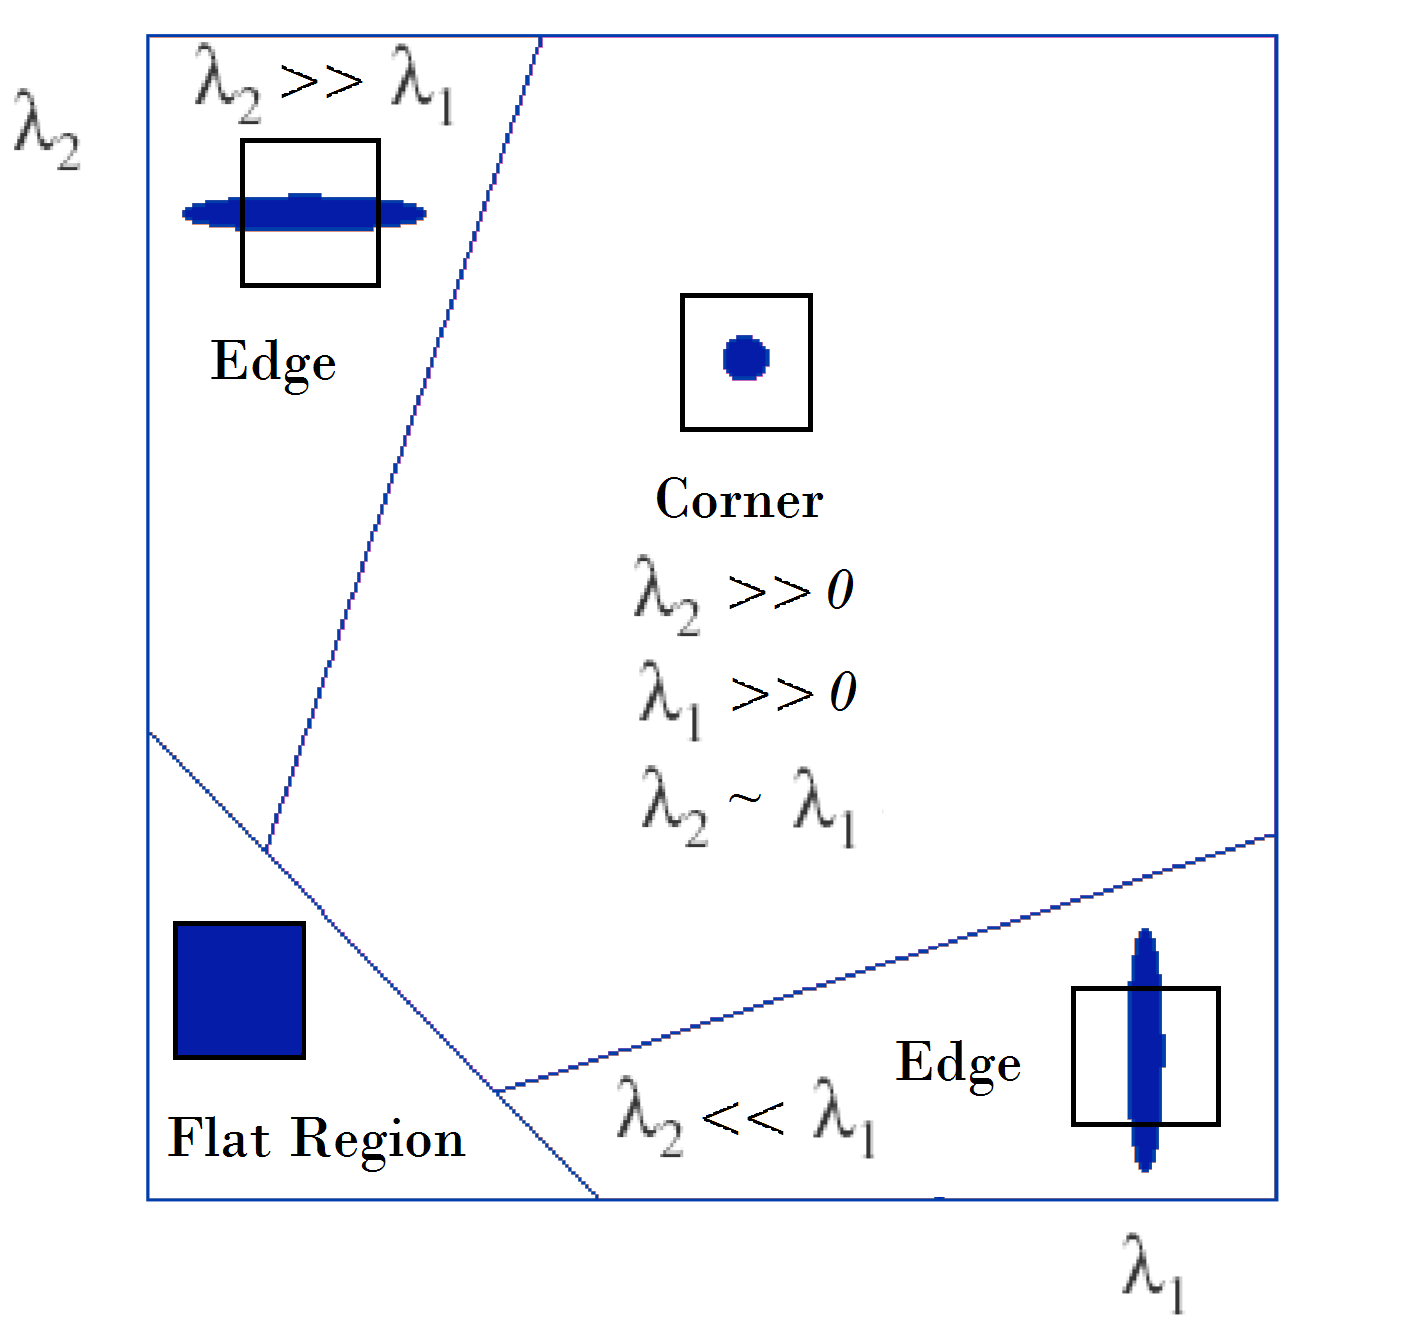
\includegraphics[width=0.6\linewidth]{lucasKanade/harrisMillora.png}
%\caption{Eigenvalues response for different regions .} \label{corner}
%\end{figure}




%There are several algorithms that use in different ways this eigenvalues:

\begin{itemize}

\item Harris \cite{harris}, they propose a corner detection response function. So for each pixel, they compute a matrix $M$ and with it, they compute the function
R, $R = det(M)-a \hspace{0.1cm} trace^{2}(M)$. if R is large, that pixel is a corner, if R is negative with larger magnitude, it is a an edge, and if R is small it is a 
flat region. So the they a treshold to classify those pixels as a corner. 

\item Shi-Tomasi \cite{shi}, they define the \textit{cornerness} in another way. The image has a maximum value ( e.g. 255), so $\lambda_{1}$, $\lambda_{2}$ also have an upper bound, then it is only necessary to check that $min(\lambda_{1},\lambda_{2})$ is large enough, this is how they define \textit{cornerness}. This feature is called good features to track, because the authors defined a \textit{good} features those whose motion can be estimated reliably, and they reached the same conlusions as Harris. This method is implement in the OpenCV's routine \texttt{goodFeaturesToTrack()}.

\end{itemize}

\subsubsection{Motion estimation}

Now, we have invariant points, we want to estimate the motion of those points. In order to do so, we compute the optical flow. This is the apparent two-dimensional motion of birightness pattern in the image. In the next figure \ref{refArchiteOF} we visualized this idea.


\begin{figure}[H]
		
\centering

\subfigure[$I(x,y,t) $.]{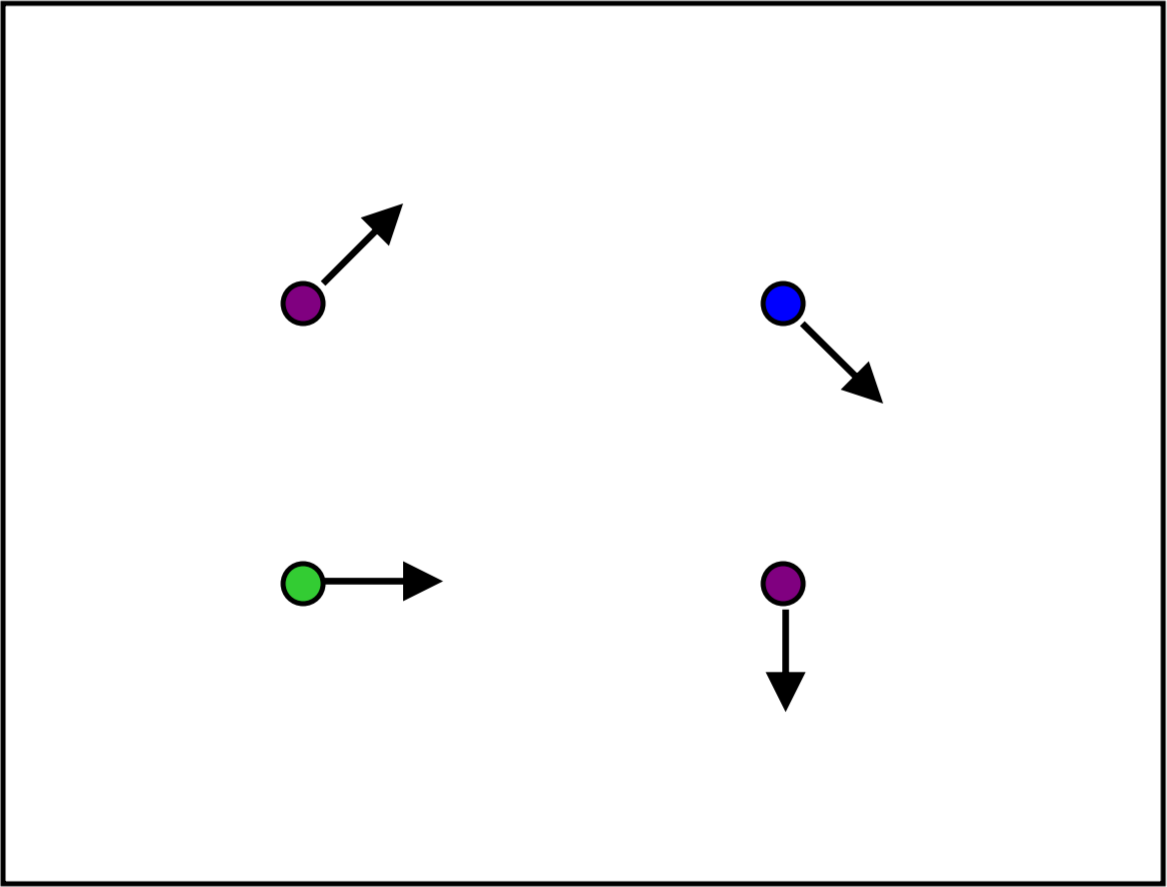
\includegraphics[width=5cm]{lucasKanade/retall1g.png}}
\subfigure[$I(x,y,t+1) $.]{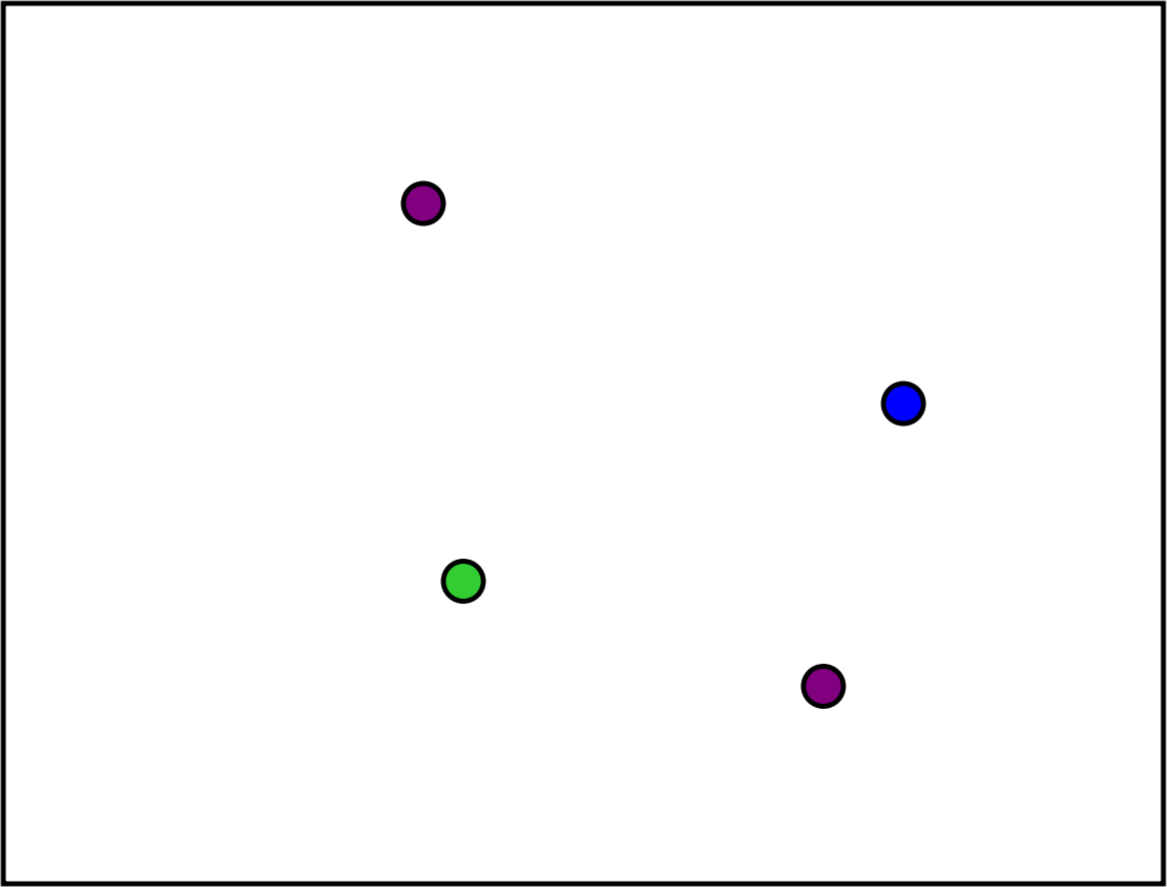
\includegraphics[width=5cm]{lucasKanade/retall2g.png}}\\


\caption{Optical flow example.}
\label{refArchiteOF}
\end{figure}

So, the question is: How do we estimate pixel motion from image $I(x,y,t)$ to image $I(x,y,t+1)$. We need to solve the pixel corresponde problem. Given a pixel in $I(x,y,t)$, look for nearby pixels of the same color in $I(x,y,t+1)$. Solving this problem is what is referred as the optical flow problem. By nearby pixels and same colour we have two assumptions:

\begin{itemize}

\item Colour constancy: a point in $I(x,y,t)$ looks the same in $I(x',y',t+1)$. For grayscale images, this is called \textit{Brightness constancy constraint}. Stated in mathematical formulation:

$$ I(x,y,t) = I(x+u,y+v,t+1) $$

$$ 0 = I(x+u,y+v,t+1)-I(x,y,t)  $$

\item Small motion: Subsequents points do not move very far, so we can estimate the motion by Taylor expansion: 

$$ I(x+u,y+v) 	\approx  I(x,y) + \dfrac{ \partial I}{\partial x}u +\dfrac{ \partial I}{\partial y}v + higher \hspace{0.1cm} order \hspace{0.1cm} terms $$


\end{itemize}
 
Then, combining these two equations, we get:

$$ 0 	\approx  I(x,y,t+1) + I_{x}u +I_{y}v - I(x,y,t) $$

where $I_{x} =  \dfrac{ \partial I}{\partial x}$, isolating the terms we obtain:

$$ 0 	\approx [I(x,y,t+1) - I(x,y,t)] + I_{x}u +I_{y}v $$

$$ 0 	\approx I_{t} + I_{x}u +I_{y}v $$

In the limit of $t$, $u$ and $v$ approaches zero ( asumption of small motion ), so it becomes, what it is called the the \textit{brightness constancy constraint equation}:
$$ 0 	= I_{t} + I_{x}u +I_{y}v $$

If we look closely, we realized that we have two unknowns $u,v$ and one equation. This is an underdetermined system. Intuitively, this means, that locally we can only determine the component of the flow in the gradient direction, the component of the flow parallel to an edge is unknown, this is the called the aperture problem. To recover the motion we need to add some extra constraints. There are several types of constraints to solve this problem:

\begin{itemize}

\item \textbf{Global constraint}, adding a smooth constraint to the brightness constraint, this new constraints penalizes for changes in $u$ and $v$ over the images, it assumes that the motion fields vary smoothly over the image. This approach was developed by Horn and Schunk \cite{horn}.

\item \textbf{Local constraint}, locally the motion field is almost the same, so we add the neighbpur pixels to the equation. This approach was developed by Lucas and Kanade \cite{LucasKana}.
\end{itemize}



\textbf{Local constraint}

In this thesis we use the Local constraint to solve the optical flow problem. As we stated above, we add a local constraint to get more equations, this assumes that the motion field is the same in the locallity. From the brightness constraint equation:

$$ 0 = I_{t}(p_{i}) + \nabla I(p_{i}) \hspace{0.1cm} [u \hspace{0.2cm} v]$$

Adding the neighborhood equations:

% 2

\[
\begin{bmatrix}
    I_{x}(p_{1}) & I_{y}(p_{1})  \\
    I_{x}(p_{2}) & I_{y}(p_{2})  \\
    \vdots & \vdots  \\
    I_{x}(p_{n}) & I_{y}(p_{n})
\end{bmatrix}
\begin{bmatrix}
    u \\
    v \\
\end{bmatrix}
=
\begin{bmatrix}
    -I_{t}(p_{1}) \\
    \vdots \\
    -I_{t}(p_{n}) \\
\end{bmatrix}
\]


Now, there are more equation than unknows, it is an overdetermined system, we have to solve it with the least squares technique. It is based on the optimization of the function:
%by using the pseudo inverse:
% 4
$$(A^{T}A) \hspace{0.1cm} d=A^{T} \hspace{0.1cm} b$$

Using the image notation:

% 5

\[
\begin{bmatrix}
    \sum I_{x}I_{x} & \sum I_{y}I_{x}  \\
    \sum I_{x}I_{y} & \sum I_{y}I_{y}   \\
\end{bmatrix}
\begin{bmatrix}
    u \\
    v \\
\end{bmatrix}
=
\begin{bmatrix}
    - \sum I_{x}I_{t} \\
    - \sum I_{y}I_{t} \\
\end{bmatrix}
\]



The system has a solution when $A^{t}A$ is invertible, it will be invertible when is well conditioned, this is when the ratio of the great and the small eigenvalues of the matrix is large but no too much. The matrix $A^{t}A$ in terms of image formulation is the second order matrix that we stated in the section \ref{feature} developing the \textit{cornerness}, then in order to be solvable it should have a strong gradient in both directions. After checking the invertability, we can solve the problem and extract the motion field:

% 6
$$ d = (A^{T}A)^{-1} \hspace{0.1cm}  A^{T}  \hspace{0.1cm} b  $$

Thus, using the image notation:

\[
\begin{bmatrix}
    u \\
    v \\
\end{bmatrix}
=
\begin{bmatrix}
    \sum I_{x}^{2} & \sum I_{y}I_{x}  \\
    \sum I_{x}I_{y} & \sum I_{y}^{2}   \\
\end{bmatrix}^{-1}
\begin{bmatrix}
    - \sum I_{x}I_{t} \\
    - \sum I_{y}I_{t} \\
\end{bmatrix}
\]



In practice motion is large, the assumption that it is small fails, consequently the approach using Taylor expansions. For two reasons, the linearity does not hold, in order to solve it, we apply an iterative refinement, which conists in compute the displacement, apply it to the pixels, and compute it again till it converges. The other one is there are local minimia and it will fail into it. To solve it, we need to utilize a coarse to fine approach, the idea is to use multiresolution to compute optical flow, the basic is that in a low resolution image the motion between pixels is very small and we can compute optical flow.

So, in order to do so, we use image pyramids, this consists in downsample these images to specific resolution, then in top level, we compute the motion field using the previous stated method, then 
we upsample the motion field and the images, We apply a transformation to one image according to the motion field computed in the previous level and then compute the optical flow between that 
transformed image and the other image, we apply this algorithm in al the resolutions

% image pyramids


\begin{figure}[H]
\centering         
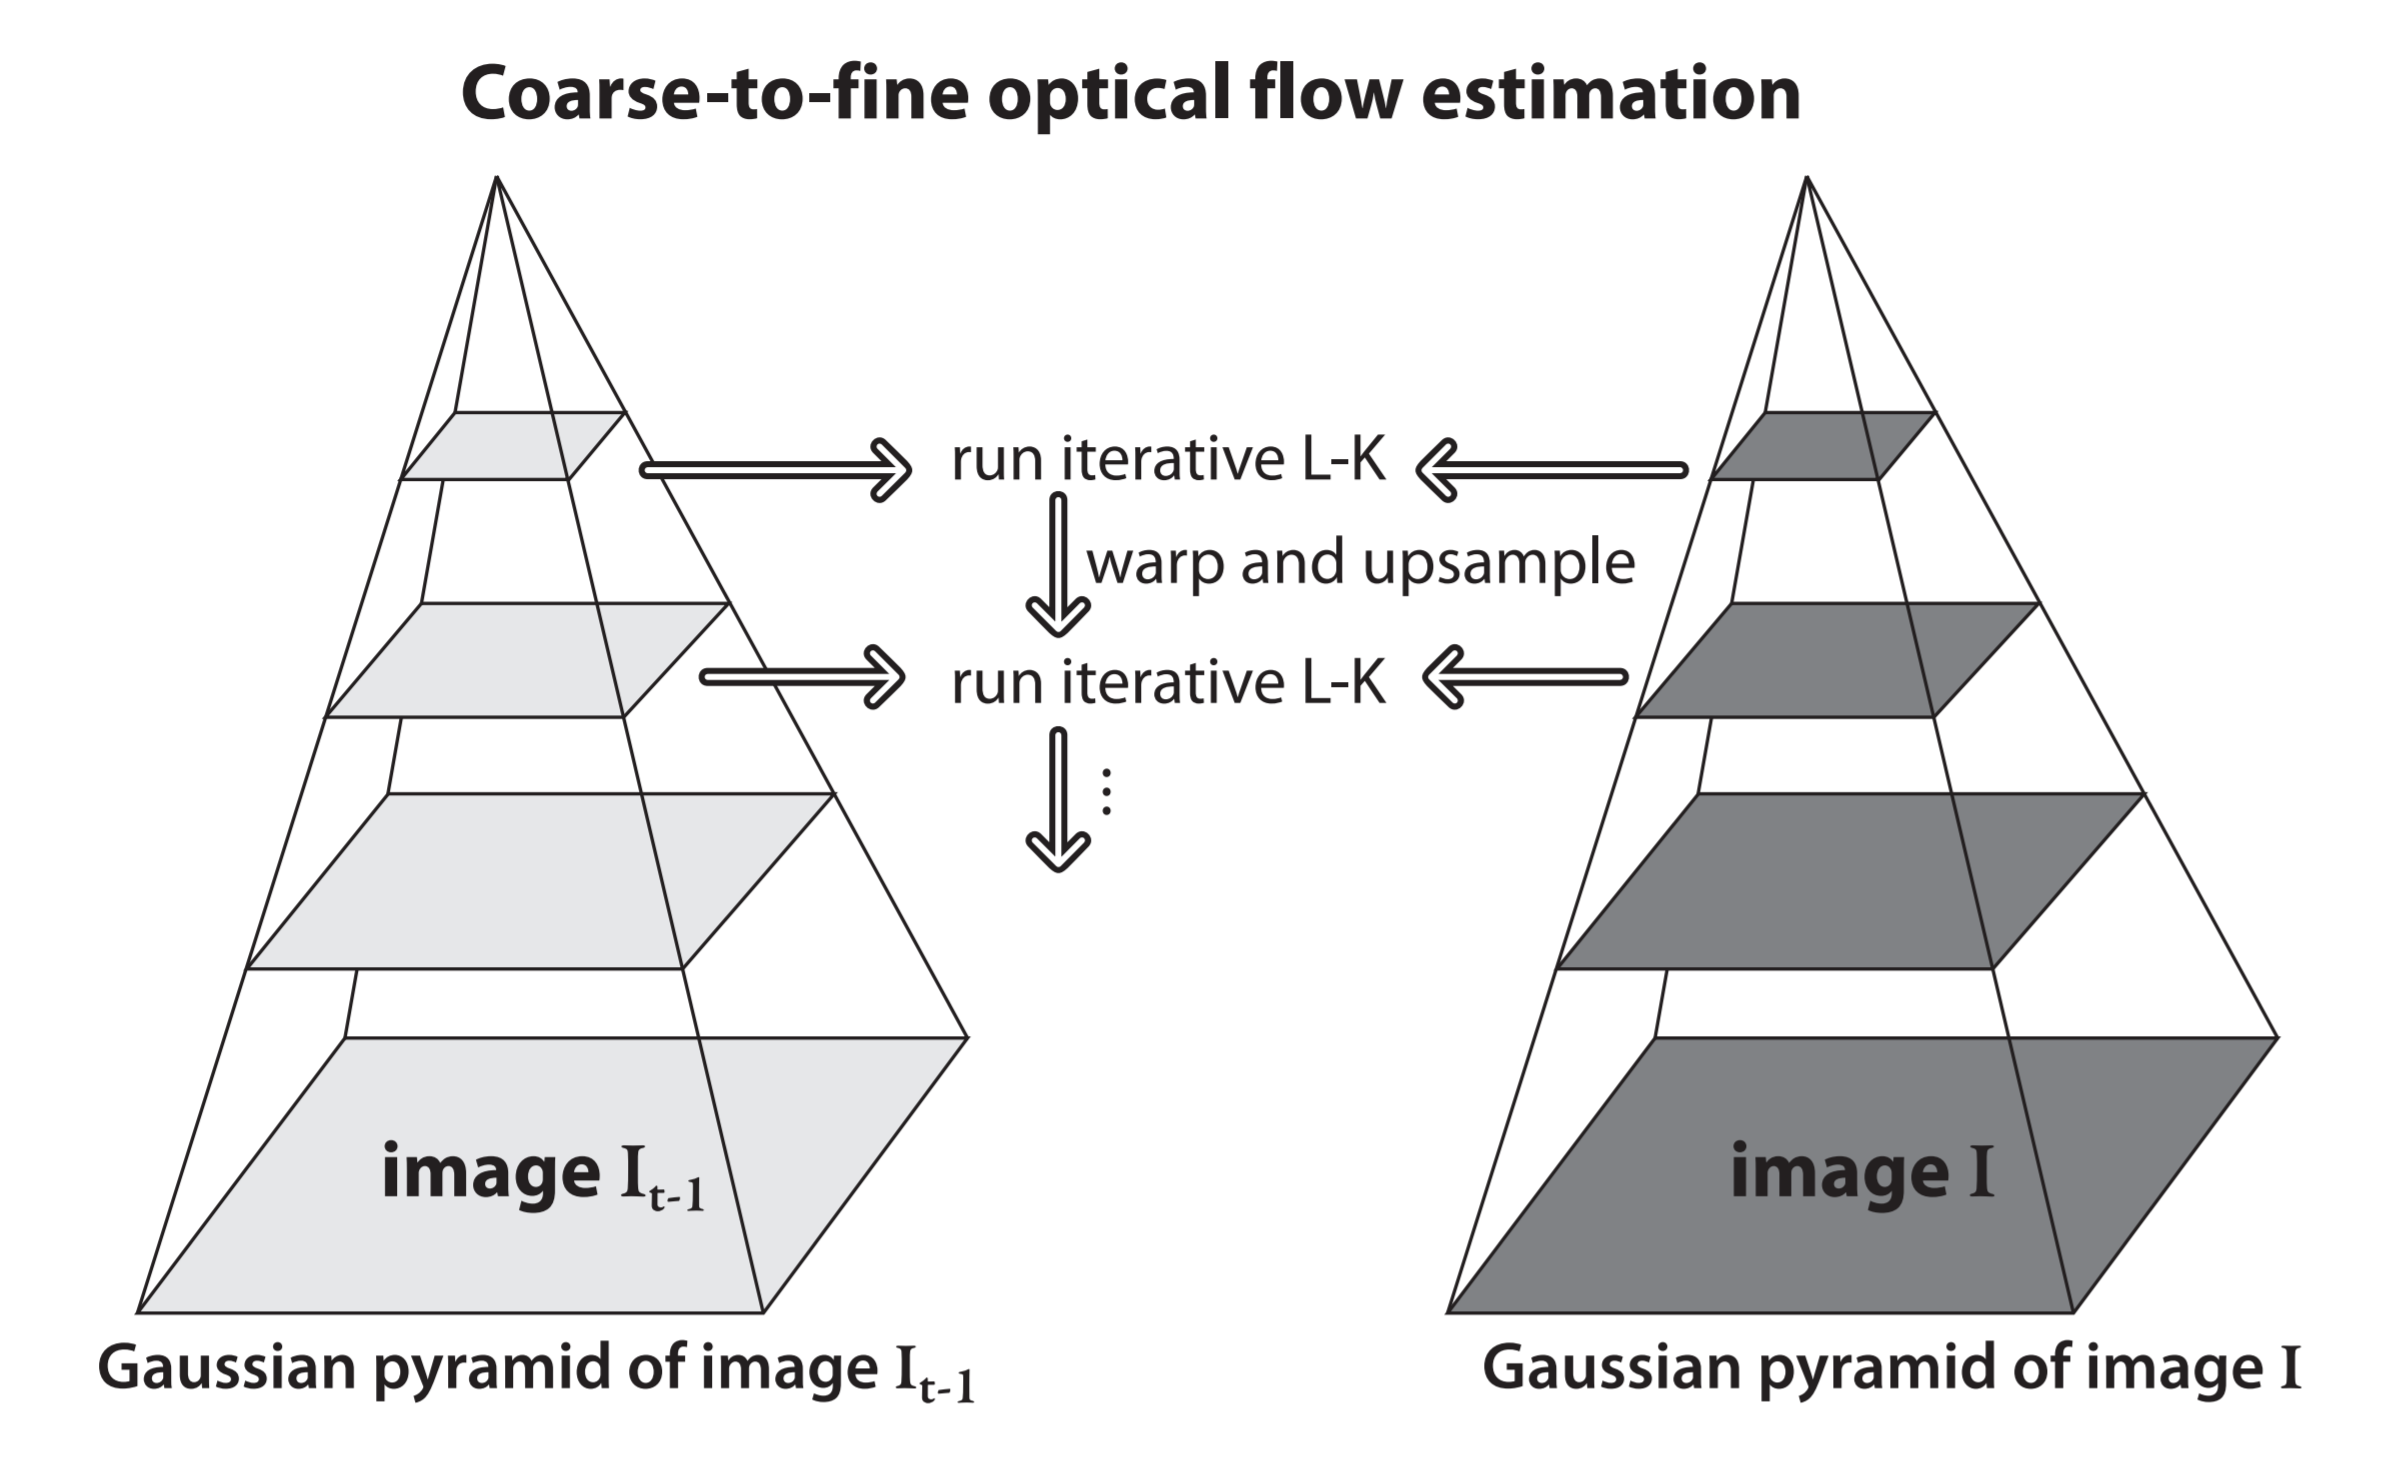
\includegraphics[width=0.6\linewidth]{lucasKanade/piram.png}
\caption{Grpahical .} \label{corner}
\end{figure}



\subsection{Person re-Identification}\label{misMatch}


After running the tracking module we might lose some trackets and in the detection step we might recover them. We need a module to check whether these have the same identity. In order to do so, we studied the methods to recover the identity with deep learning techniques.

Person identification is thoroughly studied in the field of Biometrics, it consists of  knowing one biometric characteristic, and comparing with a claiming identity query. Specifically, the topic of pedestrian identification based on images has rised in the last years, this is due to the growth of survillance applications. Also inside the topic of tracking there is a subfield called data association which studies this problem, it consists in matching trackets with further pedestrian detections.

Let's define mathematical the problem, consider $G$ is a gallery composed of $N$ images, denoted as $(g_{i})_{i=1}^{N}$. They belong to $N$ different identities $ 1,2,...,N $. Given a query image $q$, its identity is determined by:

%$$ i^{*} = argmax_{i \in 1,2,...,Ni \in 1,2,...,N} \hspace{0.5cm} sim(q,g_{i})$$

$$ i^{*} = \underset{i \in 1,2,...,N}{\arg\max} \hspace{0.5cm} sim(q,g_{i}) $$

where $i^{*}$ is the identity of probe $q$, and $sim( . , . )$ is some kind of similarity function. There are several categories of this similarity function \cite{pastPresent}:

\begin{itemize}
 
\item \textbf{Hand-crafted systems}. This involves two components, an image descriptor and a distance metric algoritm. The most common image descriptors are those used in computer visiont too, like colour \cite{lbp}, texture \cite{pairwise}, SIFT \cite{sift}, bag of word \cite{bagword}. The general idea of global metric learning is to keep all the vectors of the same class closer while pushing vectors of different classes further apart. The most commonly used formulation is based on the class of Mahalanobis distance function \cite{kiisme}, \cite{lnnn}. Other works focus on learning discriminative subspaces \cite{lda}.

\item \textbf{Deep learning techniques}. Two types of CNN models are commonly employed in the community, the first is the classification model as used in image classification, the ouptut is identity label, and the second is the siamese model using image pairs as input. The major drawback of the classification models is that they need a great quantity of training data by category, and most of the identifications datasets only provide a few examples for identity. So currently methods focus on siamese model.

\end{itemize} 

The main differences between them, is that in hand-crafted methods feature representation of the data and the metric are not learned jointly, instead, deep leraning techniques jointly optimize the representation of the input data conditioned on the \textit{similarity} measure being used \cite{EC1}. 





\subsubsection{Siamese networks}



The first work with siamese architectures were developed by LeCun \cite{siamLecun}, \cite{siameLecun2} and they adressed the identification of signatures, besides the siamese networks are used in a variaty of problems like: image recovery \cite{siameseQuer}, feature descriptor \cite{siameDescri}, comparing patches \cite{patch1}, one shot learning \cite{siameseOne}, learning visual similarity \cite{siamesSImi}. 

Siamese CNN topologies can be grouped under three main categories, depending on the point where the information from each input is combined:

\begin{itemize}

\item \textbf{Cost function}. Input patches are processed by two parallel branches featuring the same network structure and weights. Finally, the top layers of each branch are fed to a cost function.

\item \textbf{In-network}. The top layers of the parallel branches processing the two different inputs are concatenated and some more layers added on top of that. Finally, the standard softmax log-loss function is employed.

\item \textbf{Joint data input}. The two input patches are stacked together forming a unified input to the CNN. Again, the softmax log-loss function is used here.

\end{itemize}

While the two first approaches have yield good results and historically were dominant, the best perfomance is obtained with the joint data input strategy. As pointed out by  \cite{patch1} and further corroborated by \cite{patch2}, and \cite{patch3}, jointly using information form both images from the first layer tends to deliver a better perfomance. 


In the field of person re-identification, the community has used these architectures, and they also, have developed their own loss function, what is called \textit{contrastive loss}, this loss is an extension of the Hinge loss of the SVM. This loss longs for getting close similar pairs and moving away according to one defined margin, dissimilar pairs, altough, the binary cross entropy is used by the community. Also, the community has focused in the developing of the datasets, increase the size and use of different losses but there are not any landmark dataset.


There are several papers in the literature, one of the most famous is developed by Ahmed \cite{ahmed}, they used In-network architecture although in order to join to the convolutional layers, they used \textit{cross-input neighborhood differences} layer, this layer tried to increase the differences between the features of the inputs and obtain richer representation to the classification layer.

Another paper was published by Leal-Taixé \cite{lealTaixe}, they are also the authors of the MOT challenge, their network used a cost function architecture besides they used as inputs the two images and their optical flow. They used the network as part of a data association algorithm.


\section{Software implementation}

In this section, we will explain the implementation of the algorithm based on the theoretical \ref{TheoriecArch} review.

\subsection{System setup}

The developing and testing of the software has been carried out by a personal computer. This computer has a Intel Core i7 processor and 16 GB of RAM, whereas the operative system is Ubuntu 16.04 Xenial. The graphical processing unit consist in a AMD R7 M265, but its codecs are not available for our operative systems, therefore we can not take advantage of this hardware unit. For training our deep learning models we used the Amazon Web services platform, which instances is runned in operative system with a Nvidia Tesla K80 GPU. 


\subsection{System Overview}


The system consists in two threads, one responsible of the execution of the object detector and the other one, the main thread, reasponsible of the tracker. The communication between them is unilateral, the object detector thread loads into a shared buffer the detections and the main thread incorporate them when he requires it.

So, the object detector thread, reads images, proces the forward pass of the neural network and save the detections in the shared buffer, it repeats this sequence until it has processed all the predefined list of images.

In another hand, the main tread, activates the object detector thread and waits till it gets the first detection, after this, it starts the tracking algorithm. It reads the images and computes the motion of all the regions of interest. However, at beginning of each cycle it comproves whether it has newer detection to mix in. This is the main operating mode of the algorithm and it summarizes in the figure \ref{system1}. In the next sections we will develolpe in detail these parts. 

\begin{figure}[H]
		
\centering

\subfigure[Main thread.]{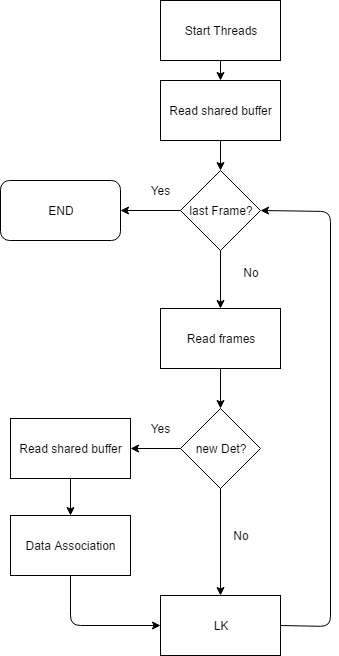
\includegraphics[width=6cm]{flows/arc.png}}
\hspace{1cm}
\subfigure[Object detector Thread.]{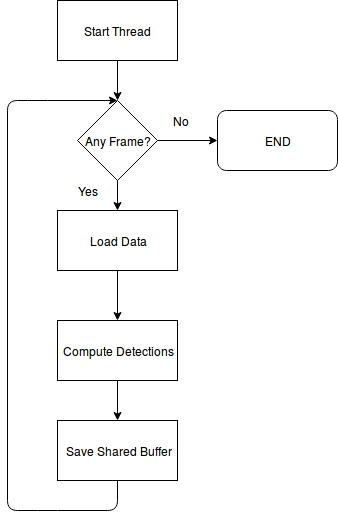
\includegraphics[width=6cm]{flows/detetc.png}}\\


\caption{Flow chart of the system.}
\label{system1}
\end{figure}





\subsection{Object detector}


As we have stated previously, the responsible of getting the detection is the object detector thread. It only read images and computes the forward pass of the network and the results are like in the figure \ref{objectDetector1}.

\begin{figure}[H]
\centering         
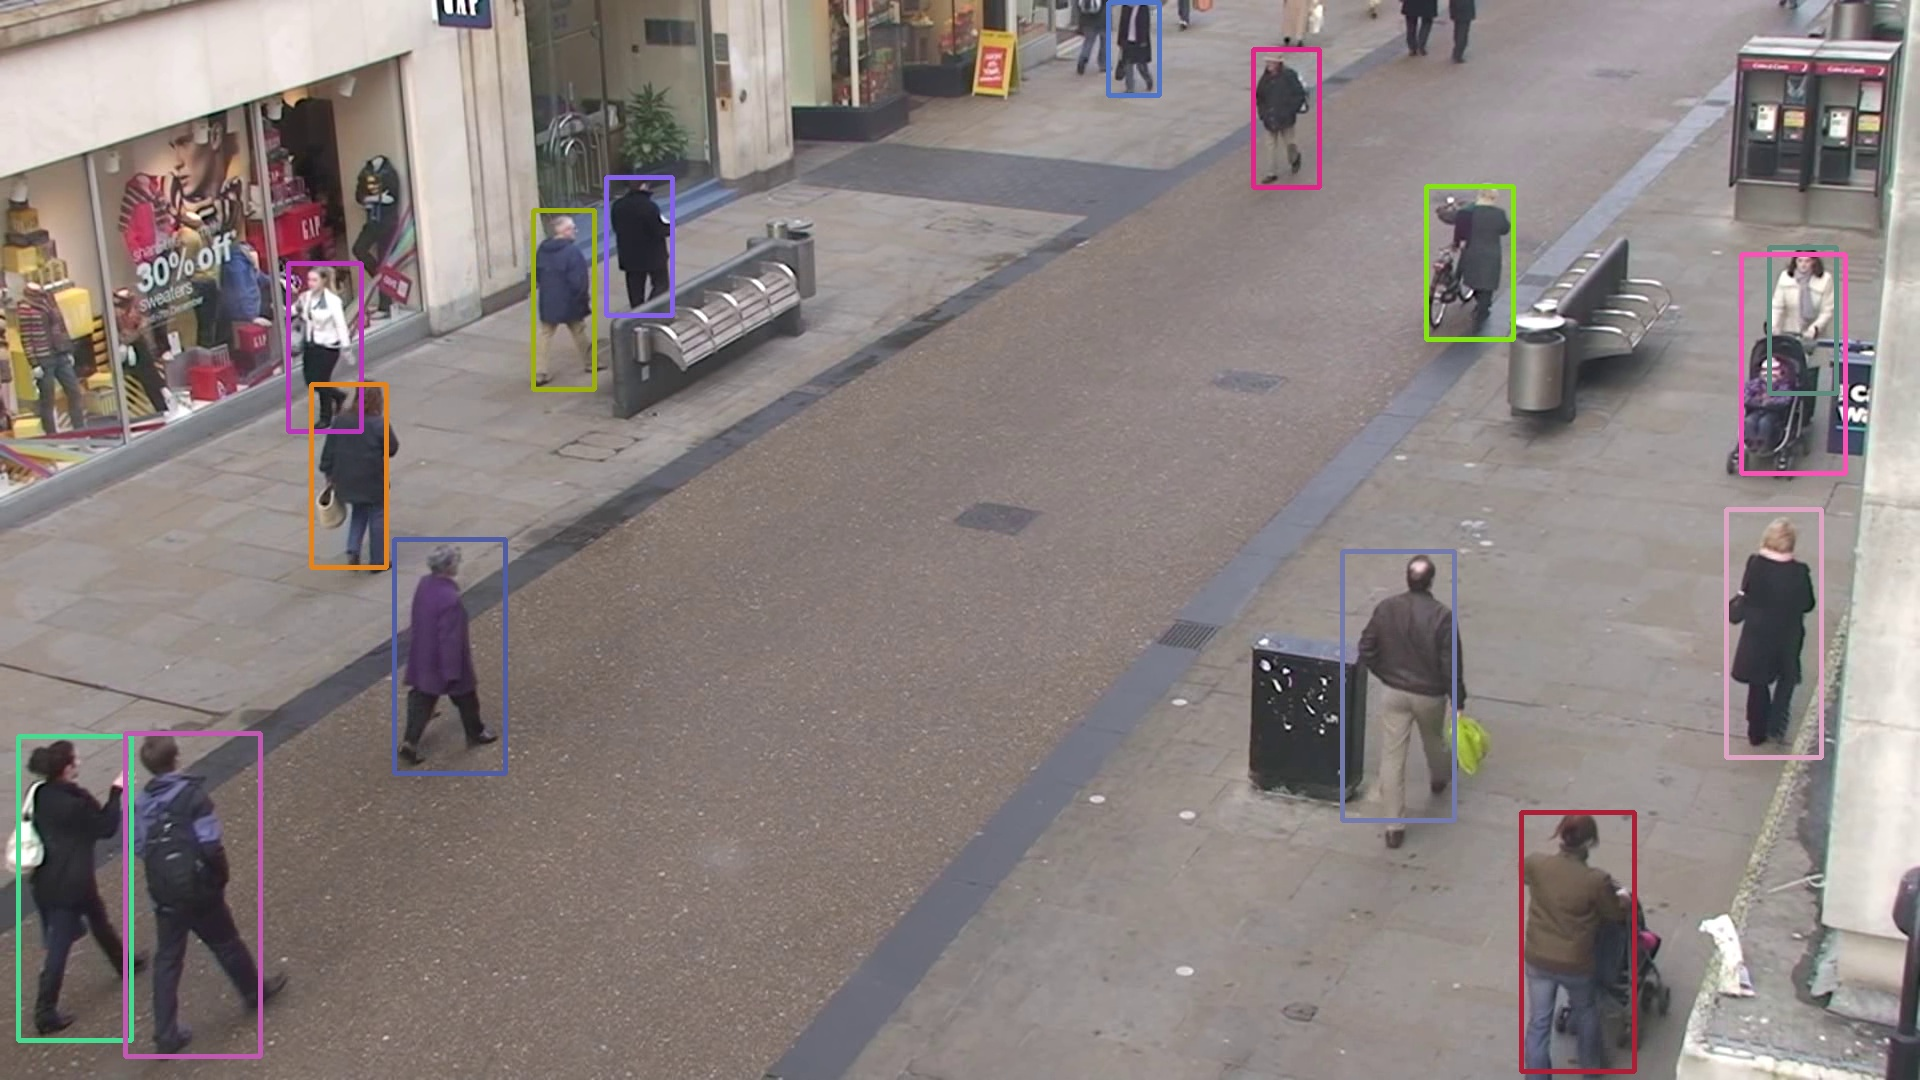
\includegraphics[width=10cm]{intro/deteccions.jpg}
\caption{Detections of the algorithm.} \label{objectDetector1}
\end{figure}



%For the choice of the detector we use the previous information of the detectors \ref{trackingBounding}, this comparision is has been done with the VOC07 challenge, particularly the perfomance detecting the person class. Also, we have extend the comprarision in the \textit{MOT16} dataset.  
%

For the choice of the detector we compare the detectors studied in the theoretical review on the \textit{MOT16} dataset. In the figure \ref{objectDetector2} we can observe the ROC curve of different detectors.


\begin{figure}[h!]
\centering         
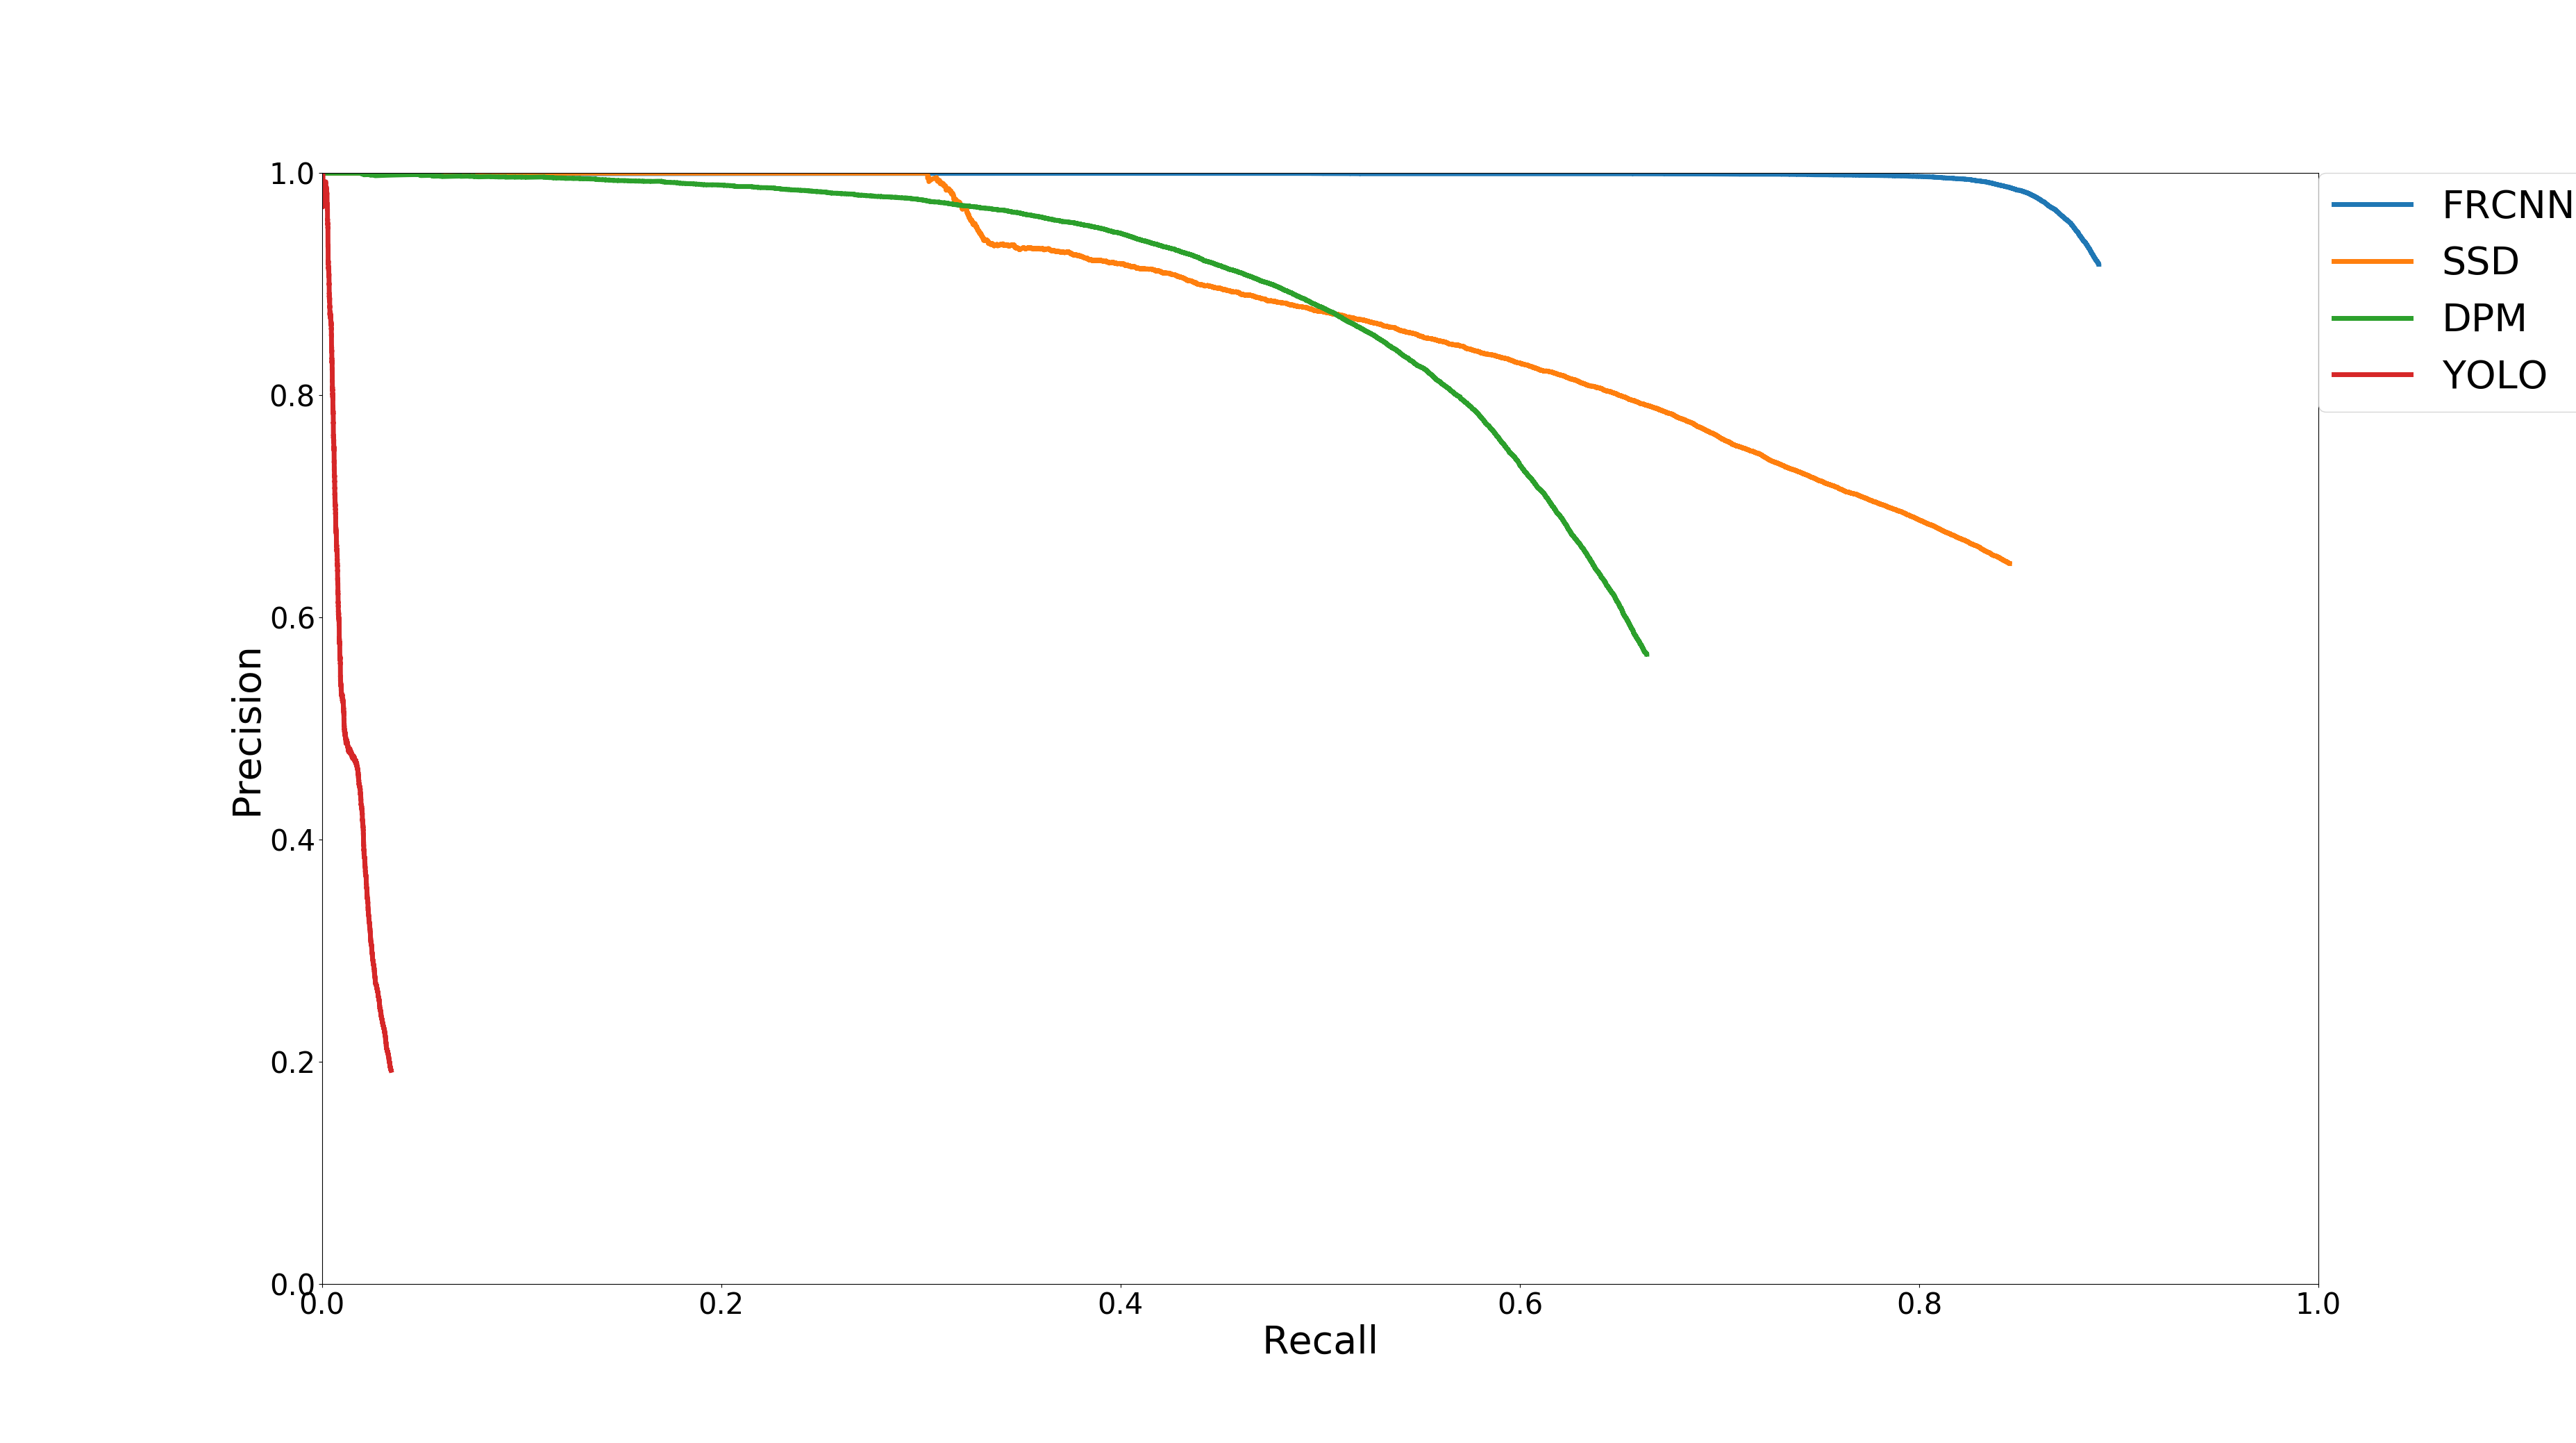
\includegraphics[width=15cm]{objectDetection/det.png}
\caption{Detections ROC curve.} \label{objectDetector2}
\end{figure}

% tablas y grafica comparación

Finally, the conclusions of the characteristics are the following:

\begin{itemize}

\item \textbf{Faster-RCNN}, it scores $0.81$ average precision on the dataset, although we could not used due a software incompabilities, it requires a Nvidia GPU to be executed.

\item \textbf{R-FCN}, the code is not publicly available.

\item \textbf{DPM}, it scores $0.69$ average precision on the dataset, although we could not used due a software incompabilities, it requires a Nvidia GPU to be executed.

\item \textbf{YOLO}, it scores $0.09$ average precision on the dataset, it takes $6$ seconds per image \cite{yoloDark}. 

\item \textbf{PVANET}, the code is not publicly available.

\item \textbf{SSD}, it scores $0.73$ average precision on the dataset, it takes $0.9$ seconds per image. We used the tensorflow version of the detector \cite{ssdCode} instead of the original code \cite{ssdCode2}.


\end{itemize}

According to these results we chose the SSD detector, as object detector on this thesis.


\subsection{Tracker}

Once we have the detections, as we have stated previously, the responsible of compute the motion of the detections is this module. First, computing the features and then extract the motion from the movement of those features, we can observe this process in the figure \ref{tracker1}.

\begin{figure}[H]
		
\centering

\subfigure[Features extraction.]{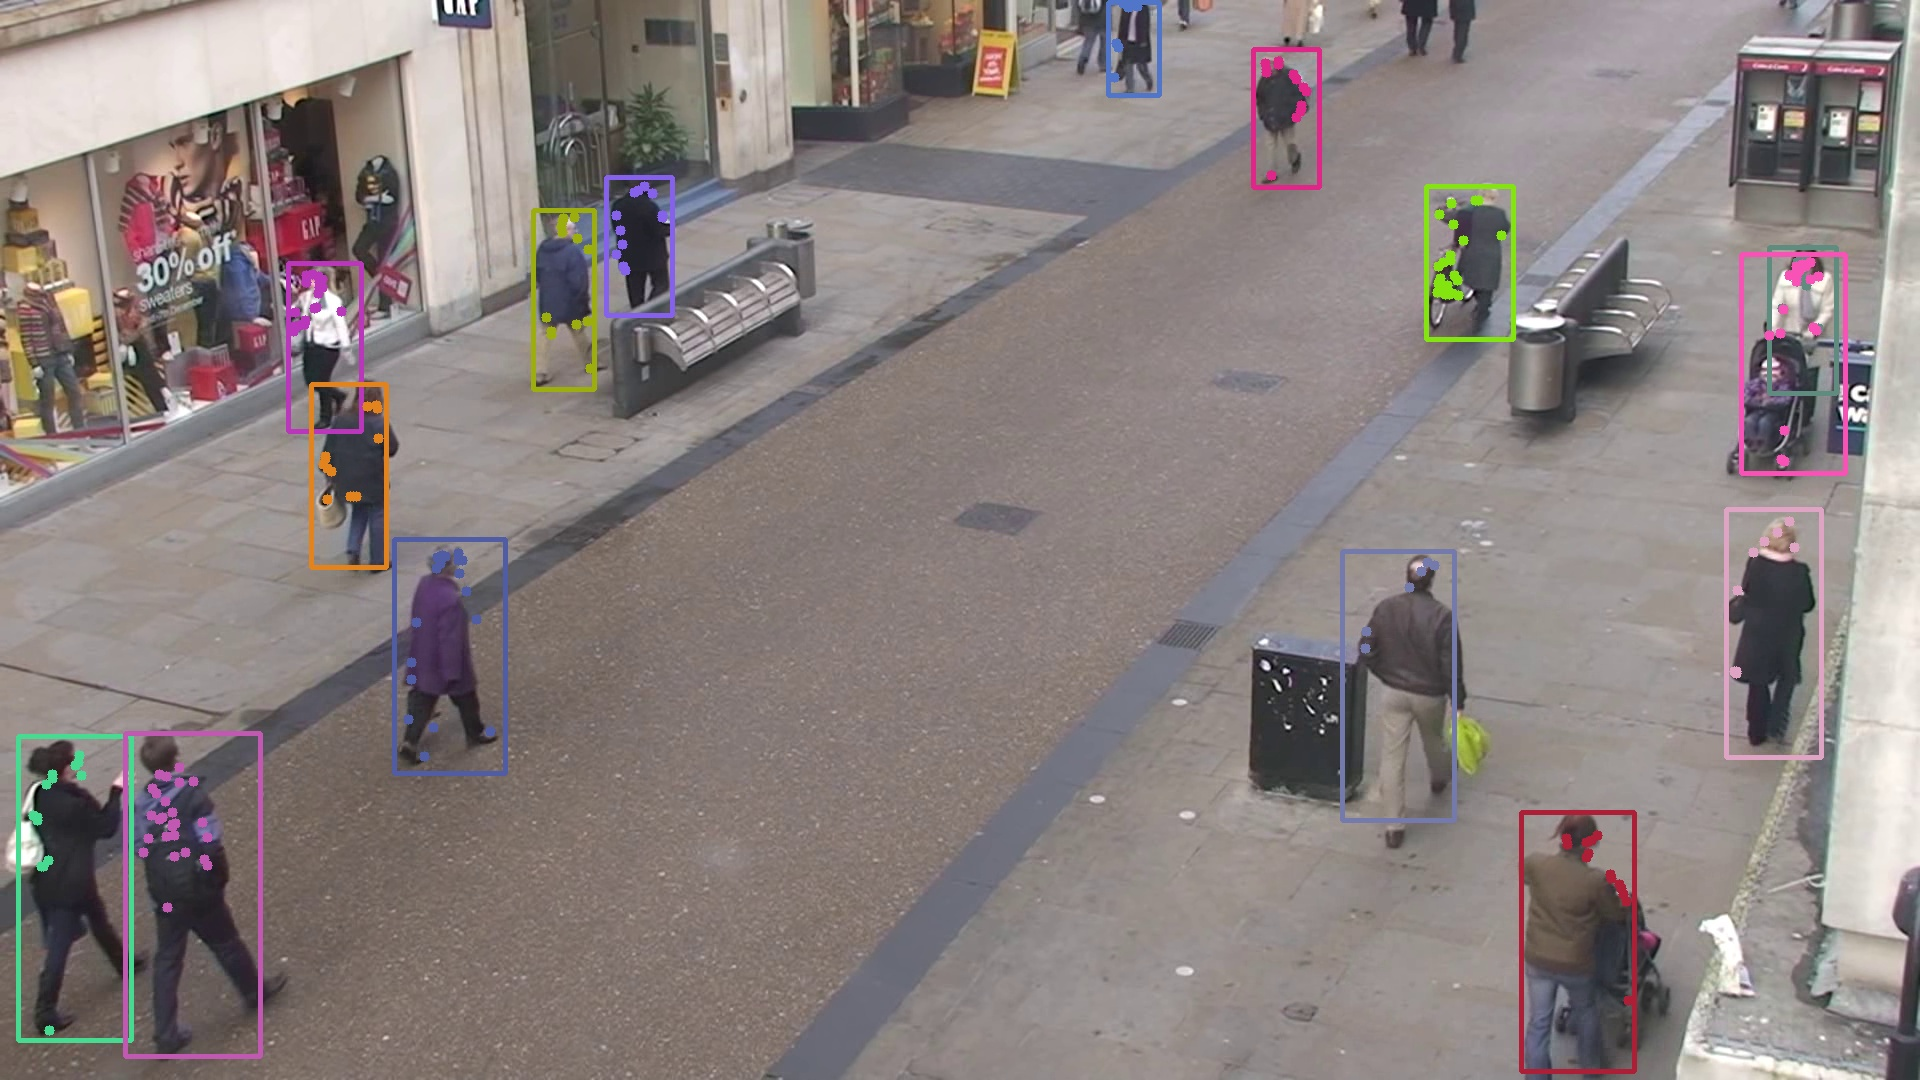
\includegraphics[width=7cm]{intro/pounts.jpg}}
\subfigure[Motion estimation.]{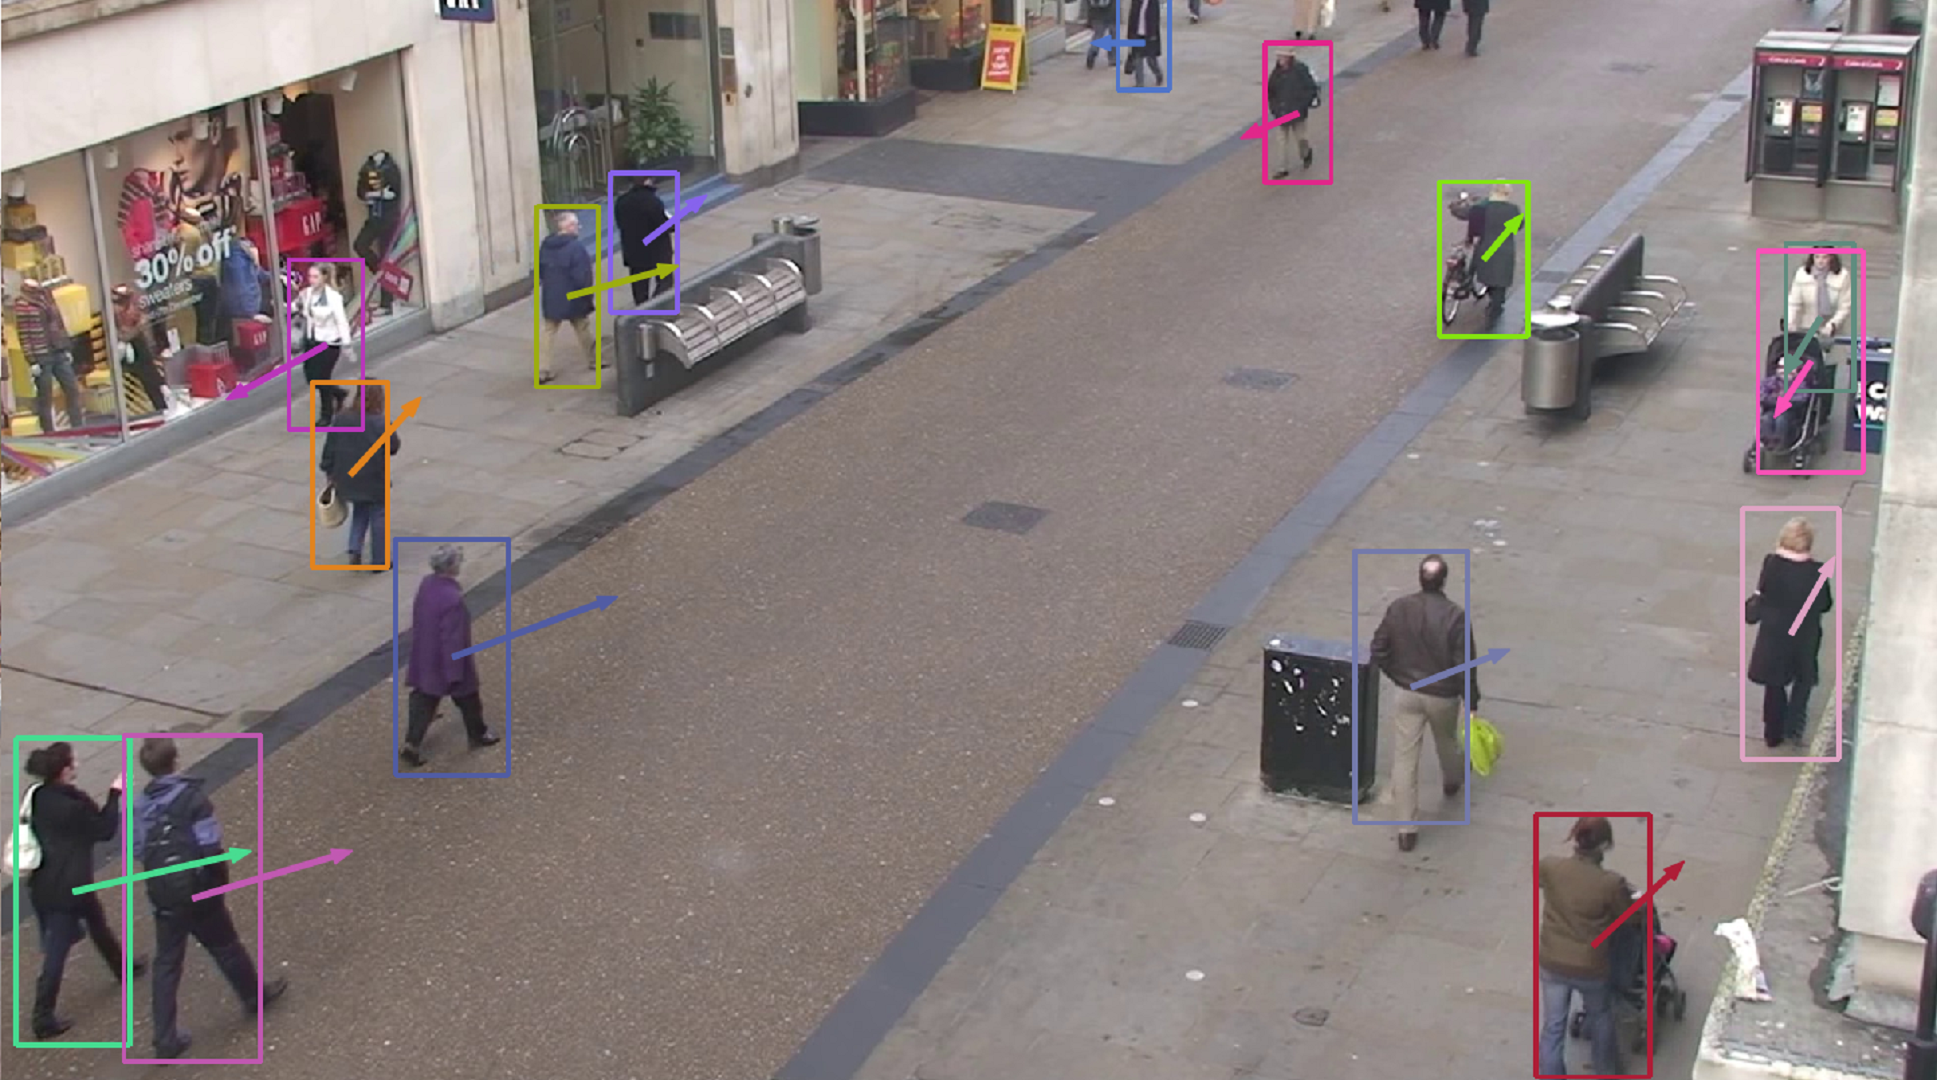
\includegraphics[width=7cm]{intro/alcover2.png}}\\


\caption{Motion computation.}
\label{tracker1}
\end{figure}



According to \cite{visualTrackingSurvey}, our method belong to tracking using matching, considering that the algorithm performs a matching of the representation of the target model built from the previous frames. We do not build an additional extended model of the appearance and merge it with the matching, instead we will apply an object detector to correct the drift of the matching.


The tracking using matching is based on the optical flow, explained in \ref{TheoriecArch}, it computes the new position through gradient descent in several frames. We will assume that the motion is pure translational. As we can observe in the sequences of frames \ref{track1w} of the dataset, the pedestrians move in translation way in the image plane, so this assumption is achieved. 


\begin{figure}[H]
\centering         
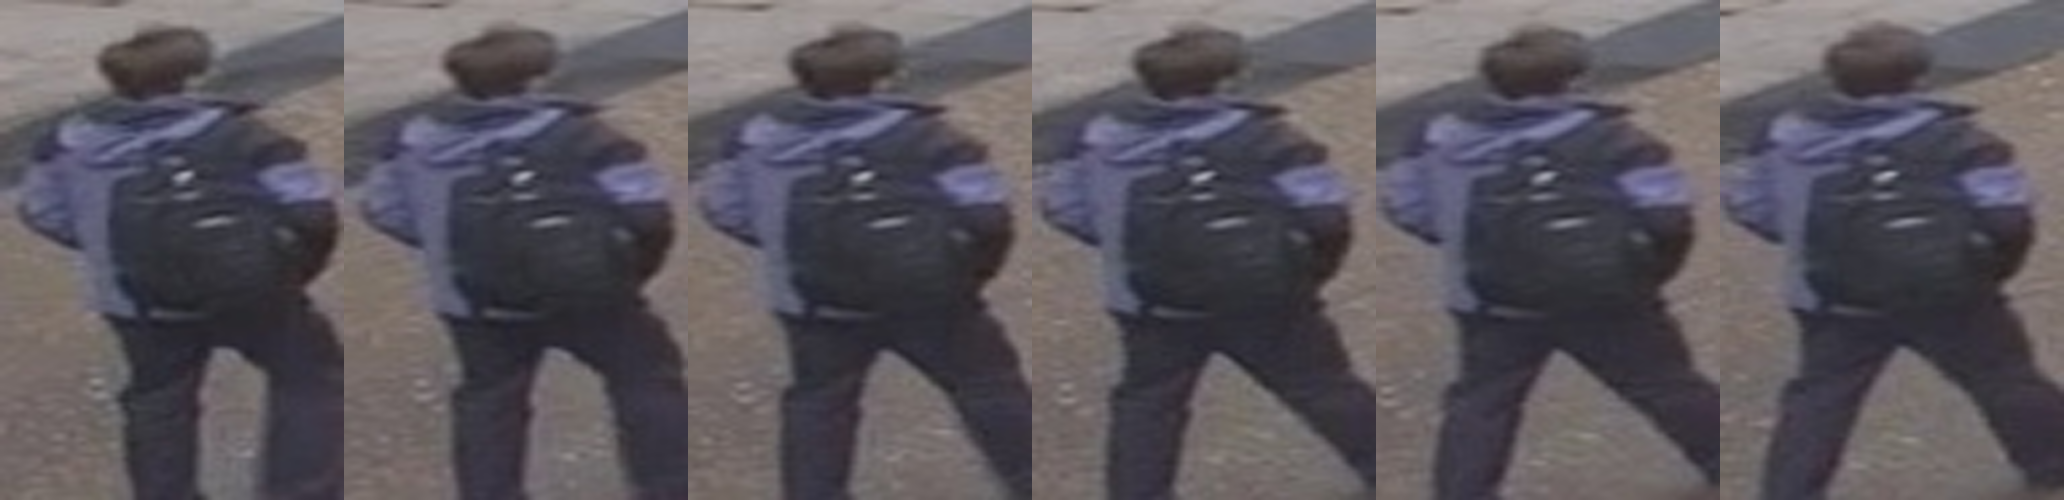
\includegraphics[width=0.9\linewidth]{changeCamera/tomeu.png}
\caption{Sequence of translational movement.} \label{track1w}
\end{figure}

In contrast to the previous figure, we can observe the next figure \ref{track2w} where the assumption of translation motion is not fulfilled ( this sequences does not belong to the used dataset, only showed to contrast the previous idea) and a translational assumption will failed.

\begin{figure}[H]
\centering         
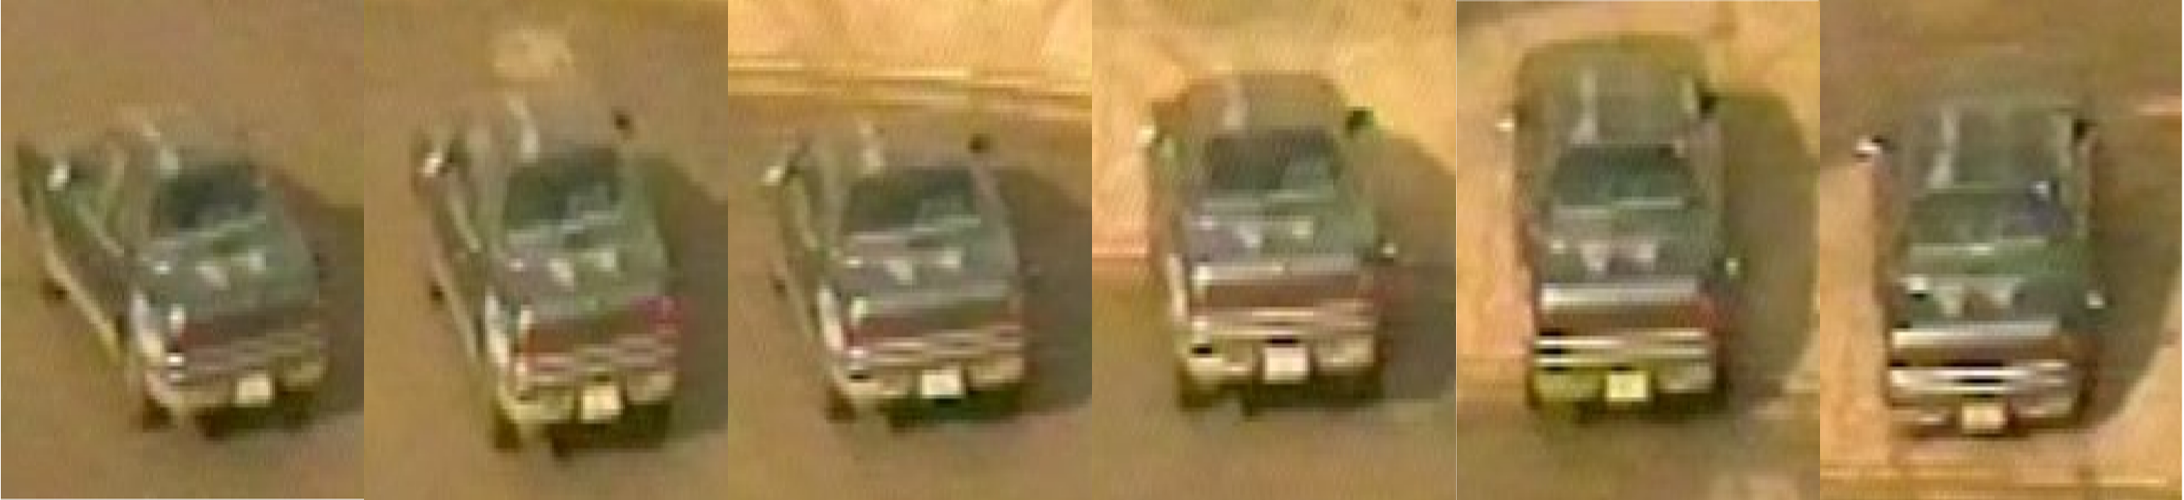
\includegraphics[width=0.9\linewidth]{changeCamera/out2.png}
\caption{Sequence of no translational movement.} \label{track2w}
\end{figure}




The tracking module is inspired by the well-known tracking algorithm \textit{MedianFlow} by Zalal et al\cite{medianFlow} with his correspondent implementation in Python\cite{medianFlowPython}. Next we explain the tracking module in details.


\subsubsection{Preprocessing and feature extractor}


For extracting the features, we use the OpenCV routine \texttt{goodFeaturesToTrack()}, this function determines strong corners on an image, according the Shi Tomasi method. His parameters are the following:
 
\begin{itemize}

\item \texttt{image}, input image

\item \texttt{maxCorners}, maximum number of corners to return. If there are more corners than are found, the strongest of them is returned.
\item \texttt{qualityLevel}, parameter characterizing the minimal accepted quality of image corners.
\item \texttt{minDistance}, minimum possible Euclidean distance between the returned corners.
\item \texttt{mask}, optional region of interest.
\item \texttt{blockSize}, Size of an average block for computing a derivative covariation matrix over each pixel neighborhood.
\item \texttt{useHarrisDetector},  Parameter indicating whether to use a Harris detector.
\item \texttt{k},  Free parameter of the Harris detector.

\end{itemize}
 
 
The strength of the further processing depends on the quality and quantity of this features, so in other to improve both, we apply some prepreprocessing to the image, we tried several preprocessings like sharpening, image contrast, median filter, and equalization. We can observe the features extraction after this preprocessings in figure \ref{prepoe}.


\begin{figure}[H]
\centering         
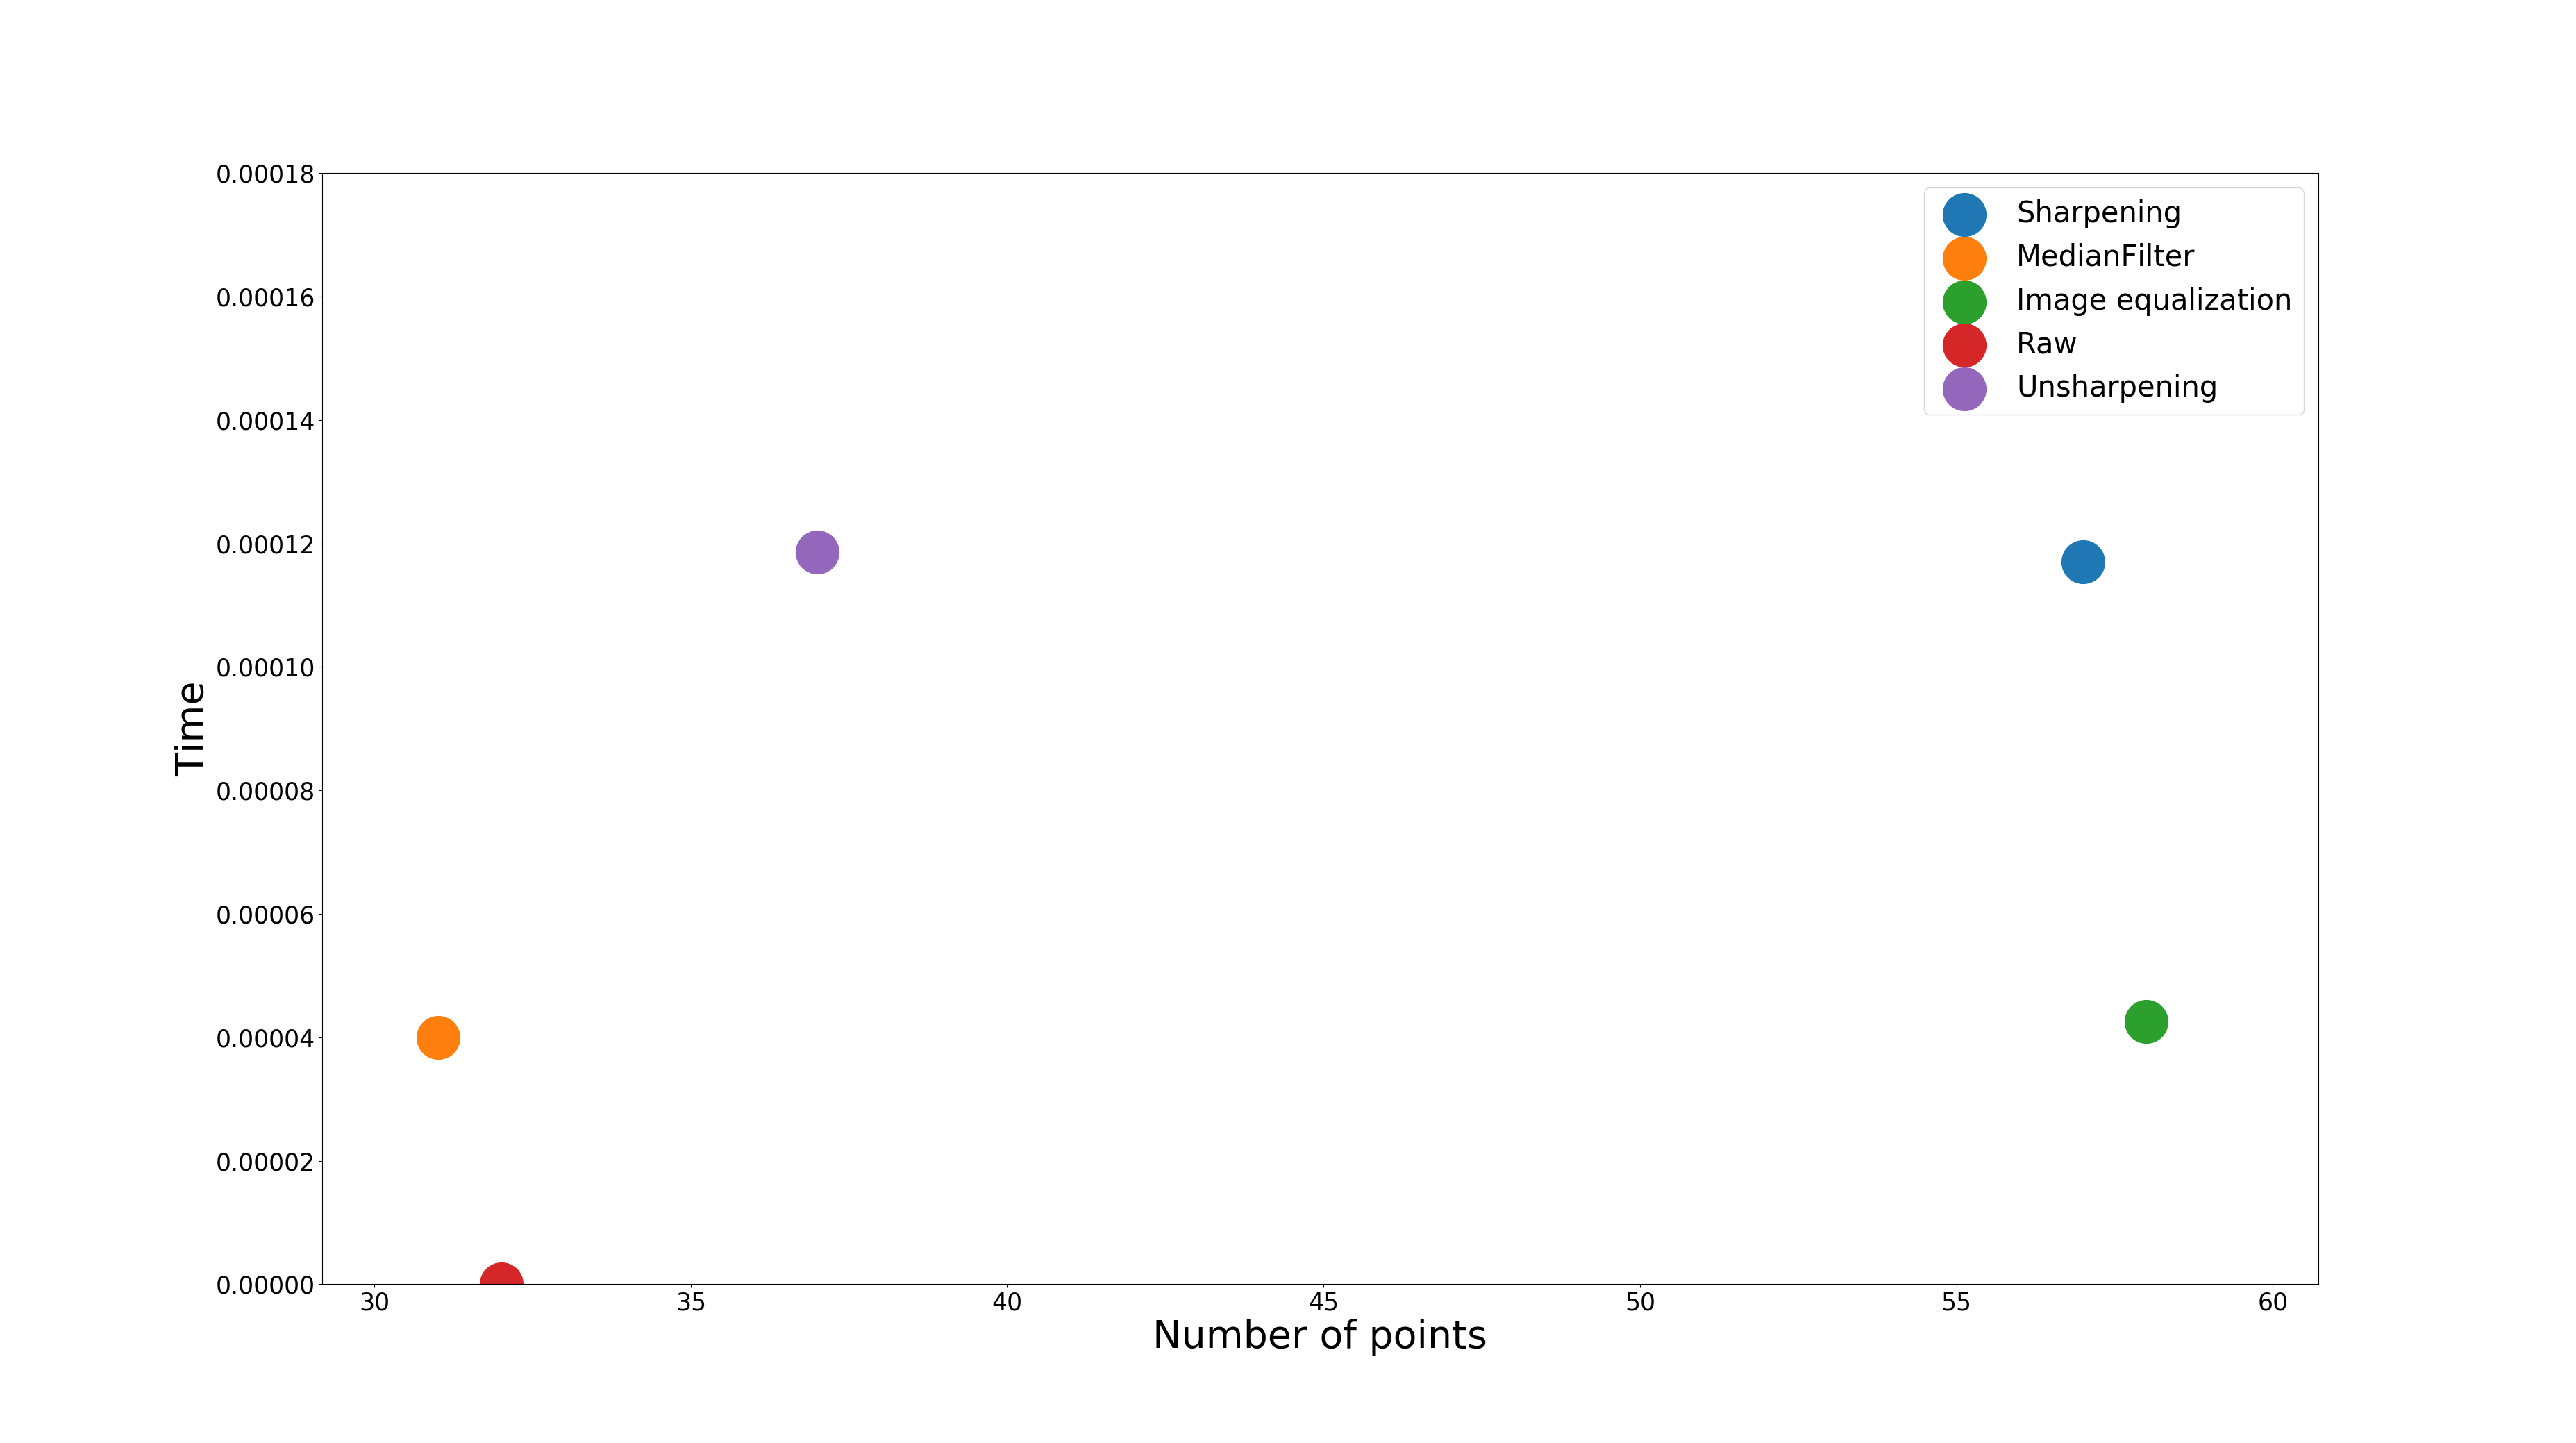
\includegraphics[width=0.9\linewidth]{tracker/preprocesing.png}
\caption{Preprocessing methods.} \label{track1w}
\end{figure}

We realized that the best preprocessing is to equalize the image, in terms of speed, it only consists in equalize an histogram and transform the image, and in terms of quality and quantity, it increases over $ 55 \%$ the number points in comparision to apply it to the raw image. In the figure \ref{prepoes} we can observe the different number of features in the raw and in the equalized image.

\begin{figure}[H]
		
\centering

\subfigure[Raw image.]{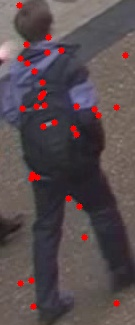
\includegraphics[width=3cm]{implementation/pointsSIN_EQU.jpg}}
\subfigure[Equalaized image.]{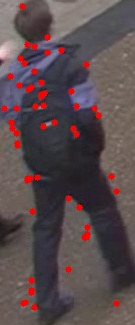
\includegraphics[width=3cm]{implementation/pointsEQU.jpg}}\\
\caption{Different preprocessings.}
\label{prepoes}
\end{figure}





\subsubsection{Motion estimation}\label{mott}

We used the lucas kanade method to matching the points. Also, we implement the same method used in \cite{medianFlow}, the proposed method is based on so called forward-backward consistency assumption that correct tracking should be independent of the direction of time-flow. Algorithmically, the assumption is exploited as follows. First, a tracker produces a trajectory by tracking the point \textit{forward} in time. Second, the point location in the last frame initializes a validation trajectory. The validation trajectory is obtained by \textit{backward} tracking from the last frame to the first one. Third, the two trajectories are compared and if they differ signicantly, the forward trajectory is considered as incorrect. \ref{motion23} illustrates the method when tracking a point between two images. Point number 1 is visible in both images and the tracker is able to localize it correctly. Tracking this point forward or backward results in identilcal trajectories. On the other hand, point number 2 is not visible in the right image and the tracker localizes a different point. Tracking this point backward ends in a different location then the original one. We also implemented the forward method.


%\begin{algorithm}
%\caption{Forward-backward method}\label{euclid}
%\begin{algorithmic}[1]
%\Procedure{FB}{}
%\State $A tracker prodcues a trajectory by tracking the point forward in time$
%\State $i \gets \textit{patlen}$
%%\BState \emph{top}:
%\If {$i > \textit{stringlen}$} \Return false
%\EndIf
%\State $j \gets \textit{patlen}$
%%\BState \emph{loop}:
%\If {$\textit{string}(i) = \textit{path}(j)$}
%\State $j \gets j-1$.
%\State $i \gets i-1$.
%\State \textbf{goto} \emph{loop}.
%\State \textbf{close};
%\EndIf
%\State $i \gets i+\max(\textit{delta}_1(\textit{string}(i)),\textit{delta}_2(j))$.
%\State \textbf{goto} \emph{top}.
%\EndProcedure
%\end{algorithmic}
%\end{algorithm}
%

\begin{figure}[H]
		
\centering

\subfigure[Image forward-backward.]{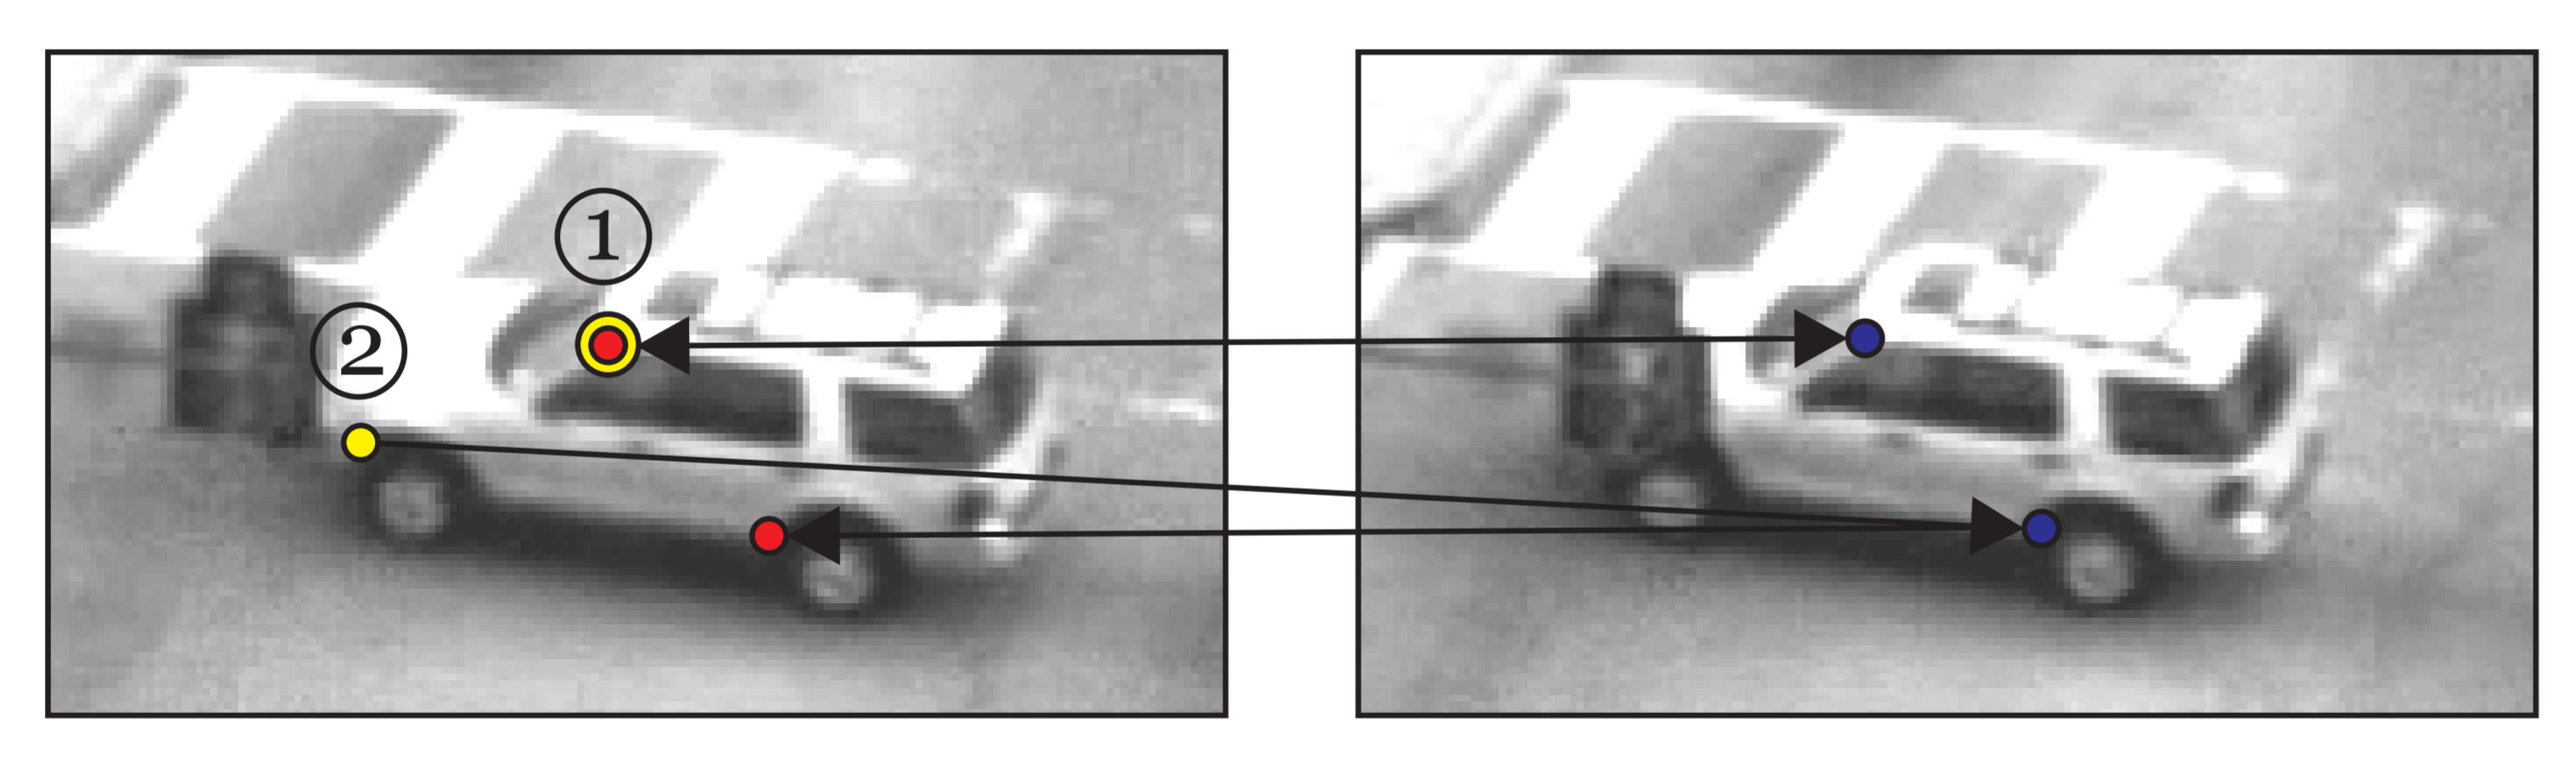
\includegraphics[width=7cm]{tracker/forwardBack.png}}
\subfigure[Scheme forward-backward.]{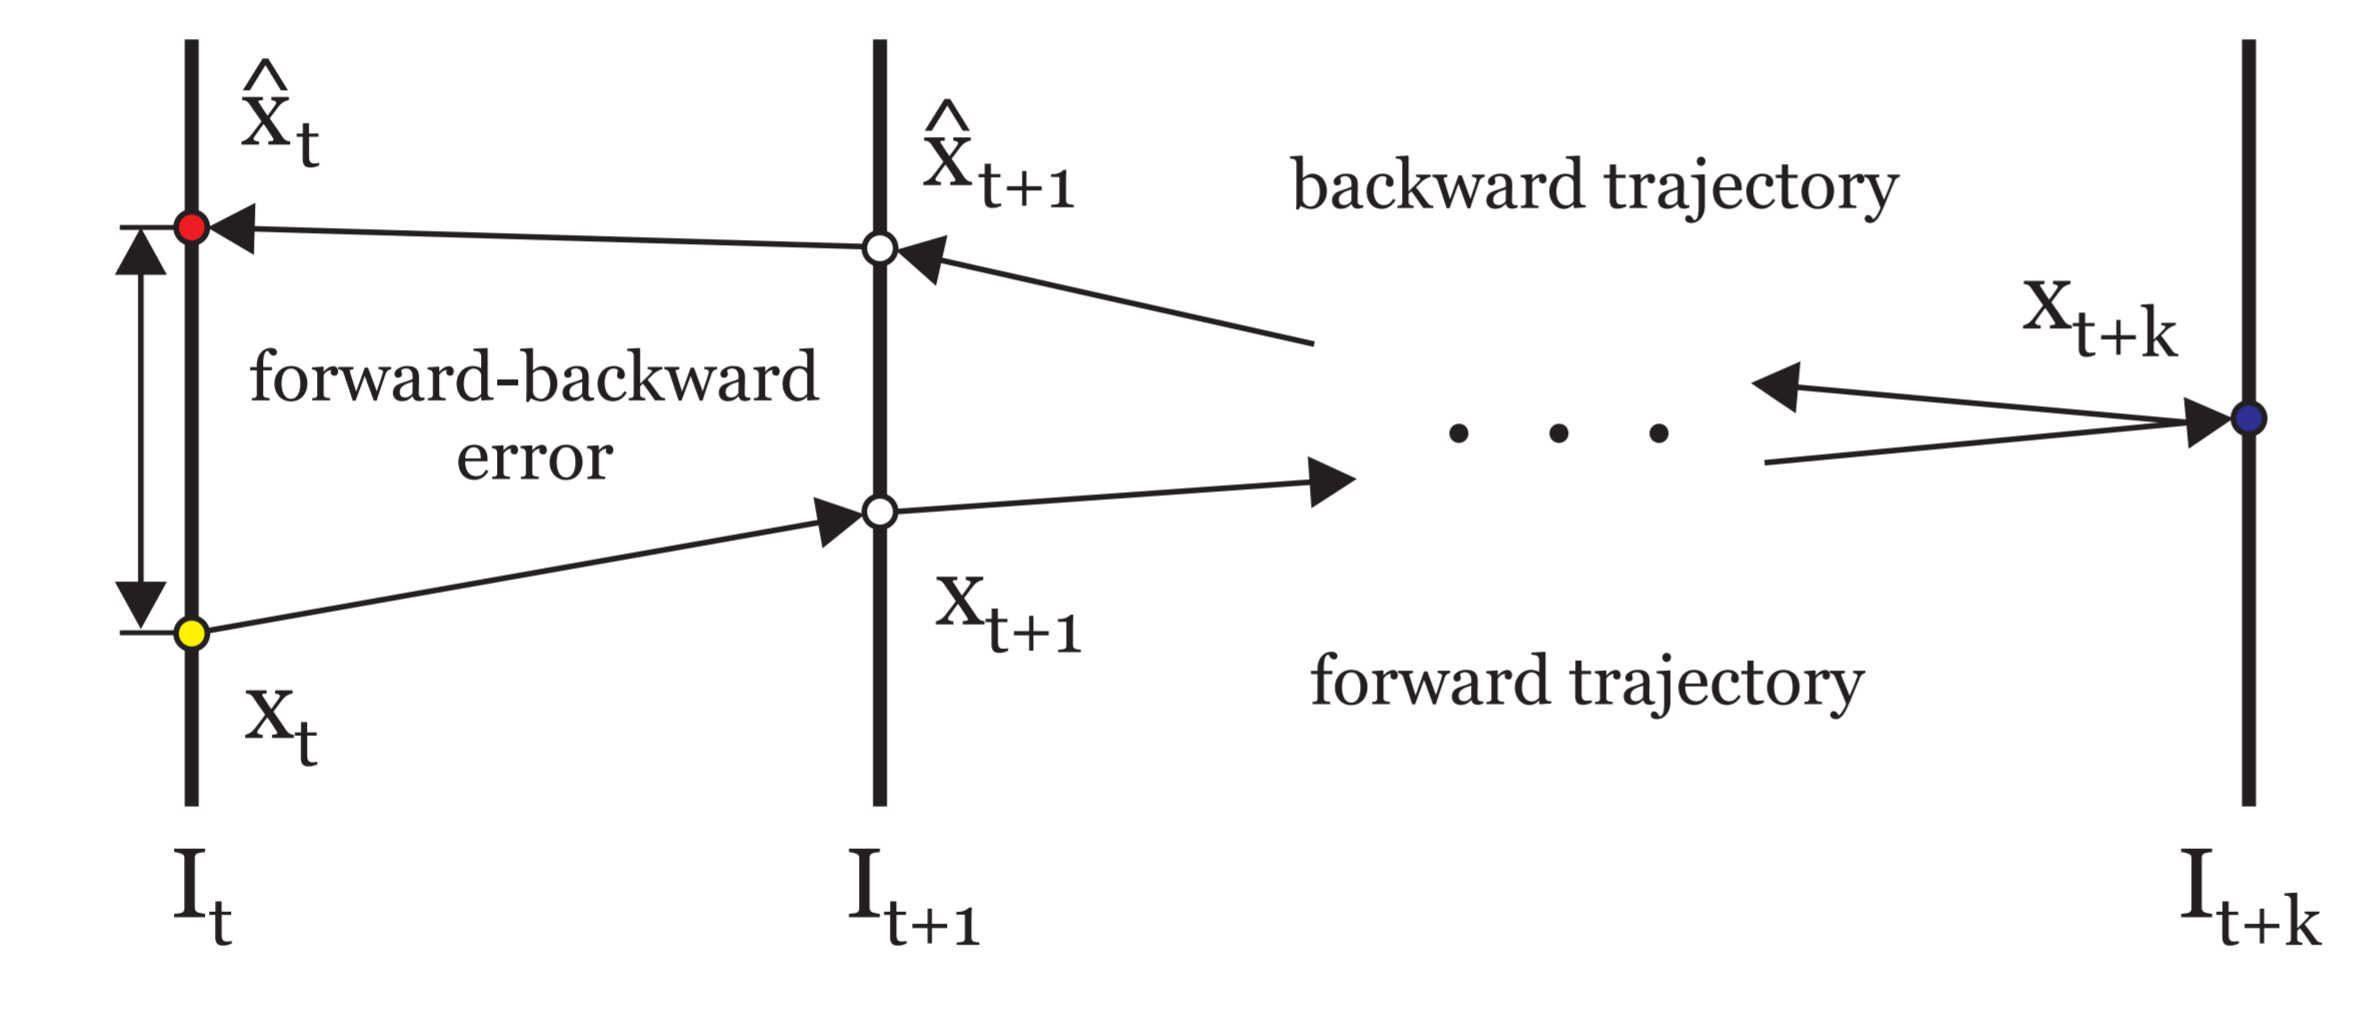
\includegraphics[width=7cm]{tracker/forwardBack2.png}}\\
\caption{Ilustration forward backward error.}
\label{motion23}
\end{figure}


To compute the matching we used the OpenCV routine \texttt{calcOpticalFlowPyrLK()}, this function implements a sparse iterative version of the Lucas-Kanade optical flow with pyramids. And his parameters are:
 
\begin{itemize}

\item \texttt{prevImg}, first image.
\item \texttt{nextImg}, second image.
\item \texttt{prevPts}, vector of 2D points for which the flow needs to be found. 
\item \texttt{nextPts}, output vector of 2D points containing the calculated new positions of input features in the second image. 
\item \texttt{status}, output status vector, it tells you whether the flow has been found.  
\item \texttt{err}, each element of the vector is set to an error for the corresponding feature.
\item \texttt{winSize}, size of the search window at each pyramid level. 
\item \texttt{maxLevel}, number of pyramid levels.  
\item \texttt{criteria}, parameter, speifying the termination criteria of the iterative search algorithm.
\end{itemize}


In the next figure we can observe the matching of the feaetues in subsequents frames.

\begin{figure}[hptb]
\centering         
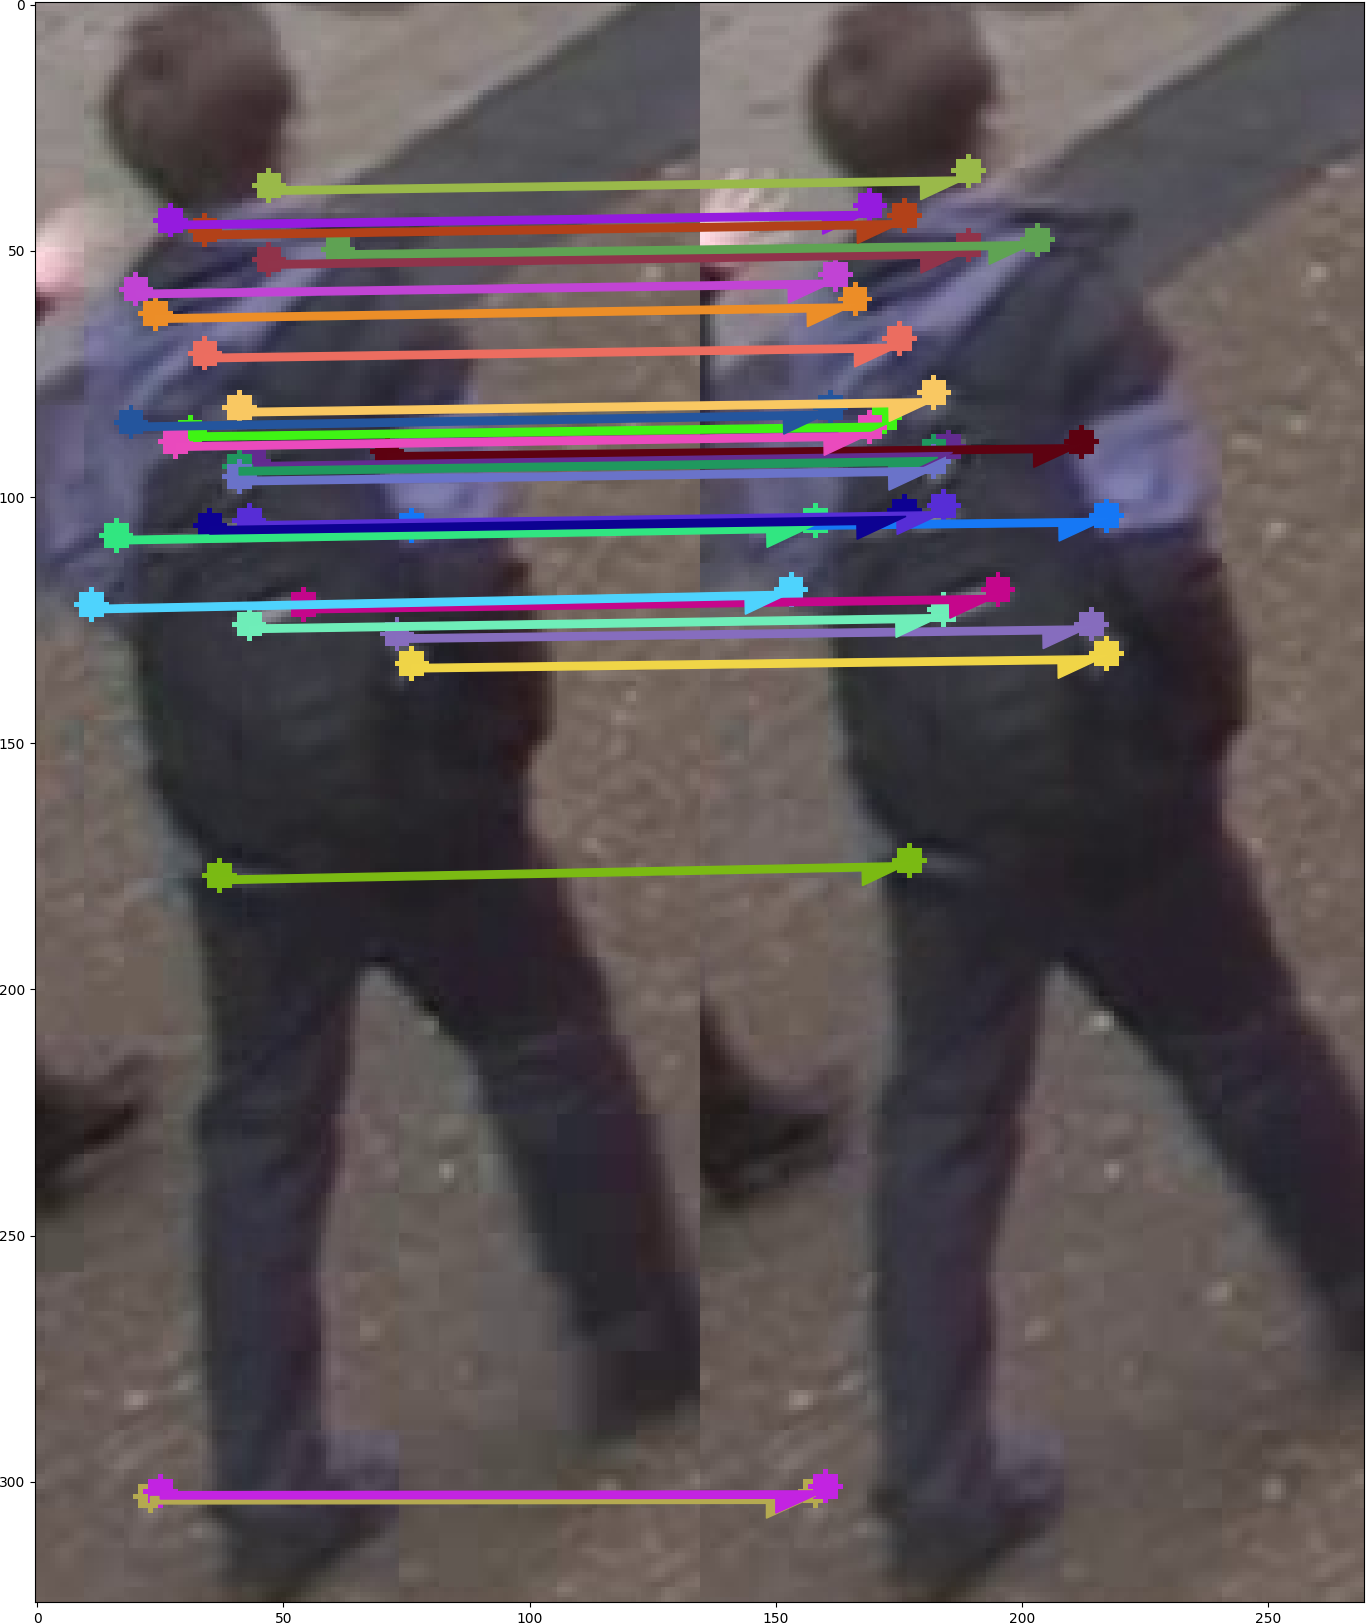
\includegraphics[width=0.3\linewidth]{implementation/matching.png}
\caption{Image and motion vectors.} \label{motion1}
\end{figure}


After this step we have a bunch of motion vectors, but some vectors in the bounding box do not belong to the person, and if we do not erase it will contribute to the motion compuation. Usually this points belong to the static elements of the frames, like the floor or urban furniture, this points in terms of motion between subsequents frames will be very low or almost statics. We can observe this fact plotting the displacement of this points and drawing it in the image, we can observe it at \ref{motion2}. So, we erase the points with a displacement smaller than a threshold. 

\begin{figure}[H]
		
\centering

\subfigure[Image points.]{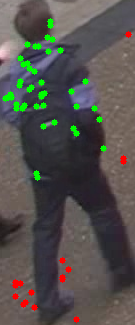
\includegraphics[width=2.5cm]{implementation/reejctMore.png}}
\subfigure[Displacement graphics.]{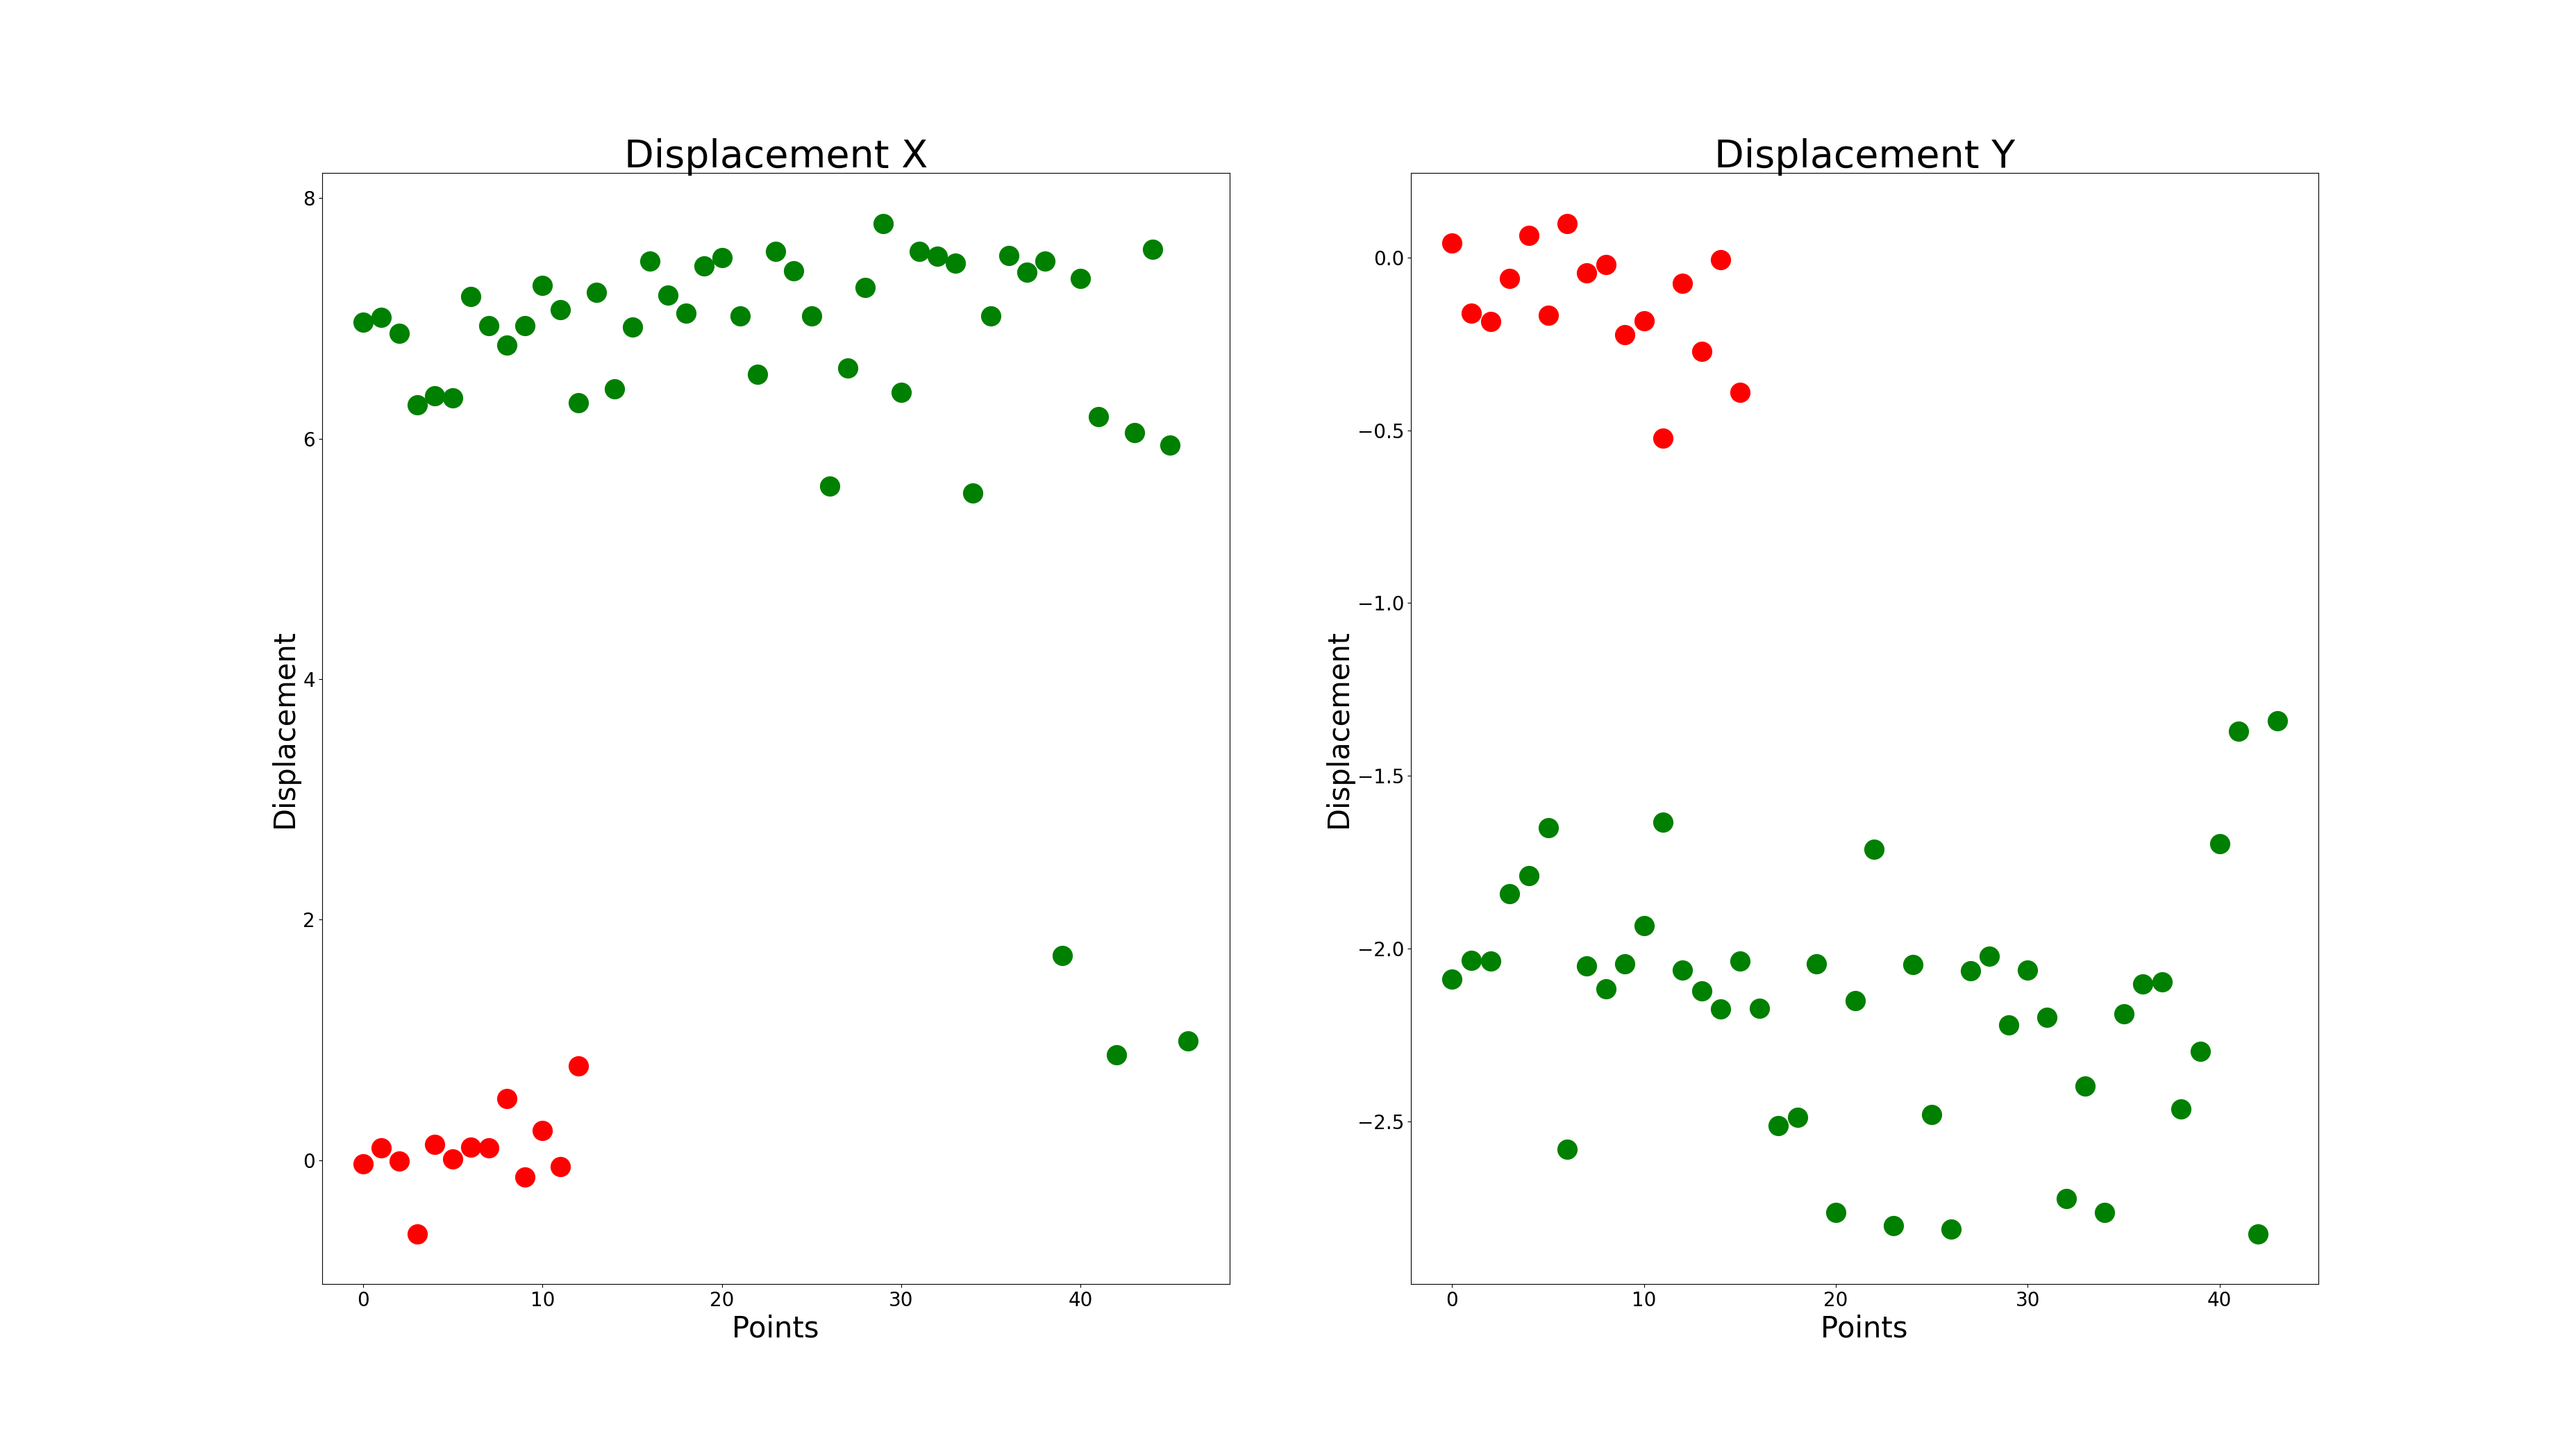
\includegraphics[width=13cm]{implementation/filterVeloPoints.png}}\\
\caption{Image and motion vectors.}
\label{motion2}
\end{figure}

But, this behavior will only work on sequences where the camera is fixed, in sequenes produced by a moving camera it will not work, we can observe the plot of displacement vectors on a sequence acquired by a moving camera \ref{motion3}. 

\begin{figure}[H]
		
\centering

\subfigure[Image points.]{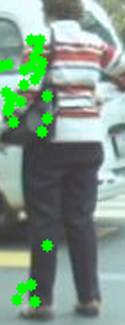
\includegraphics[width=2.5cm]{implementation/foto004.png}}
\subfigure[Displacement graphics.]{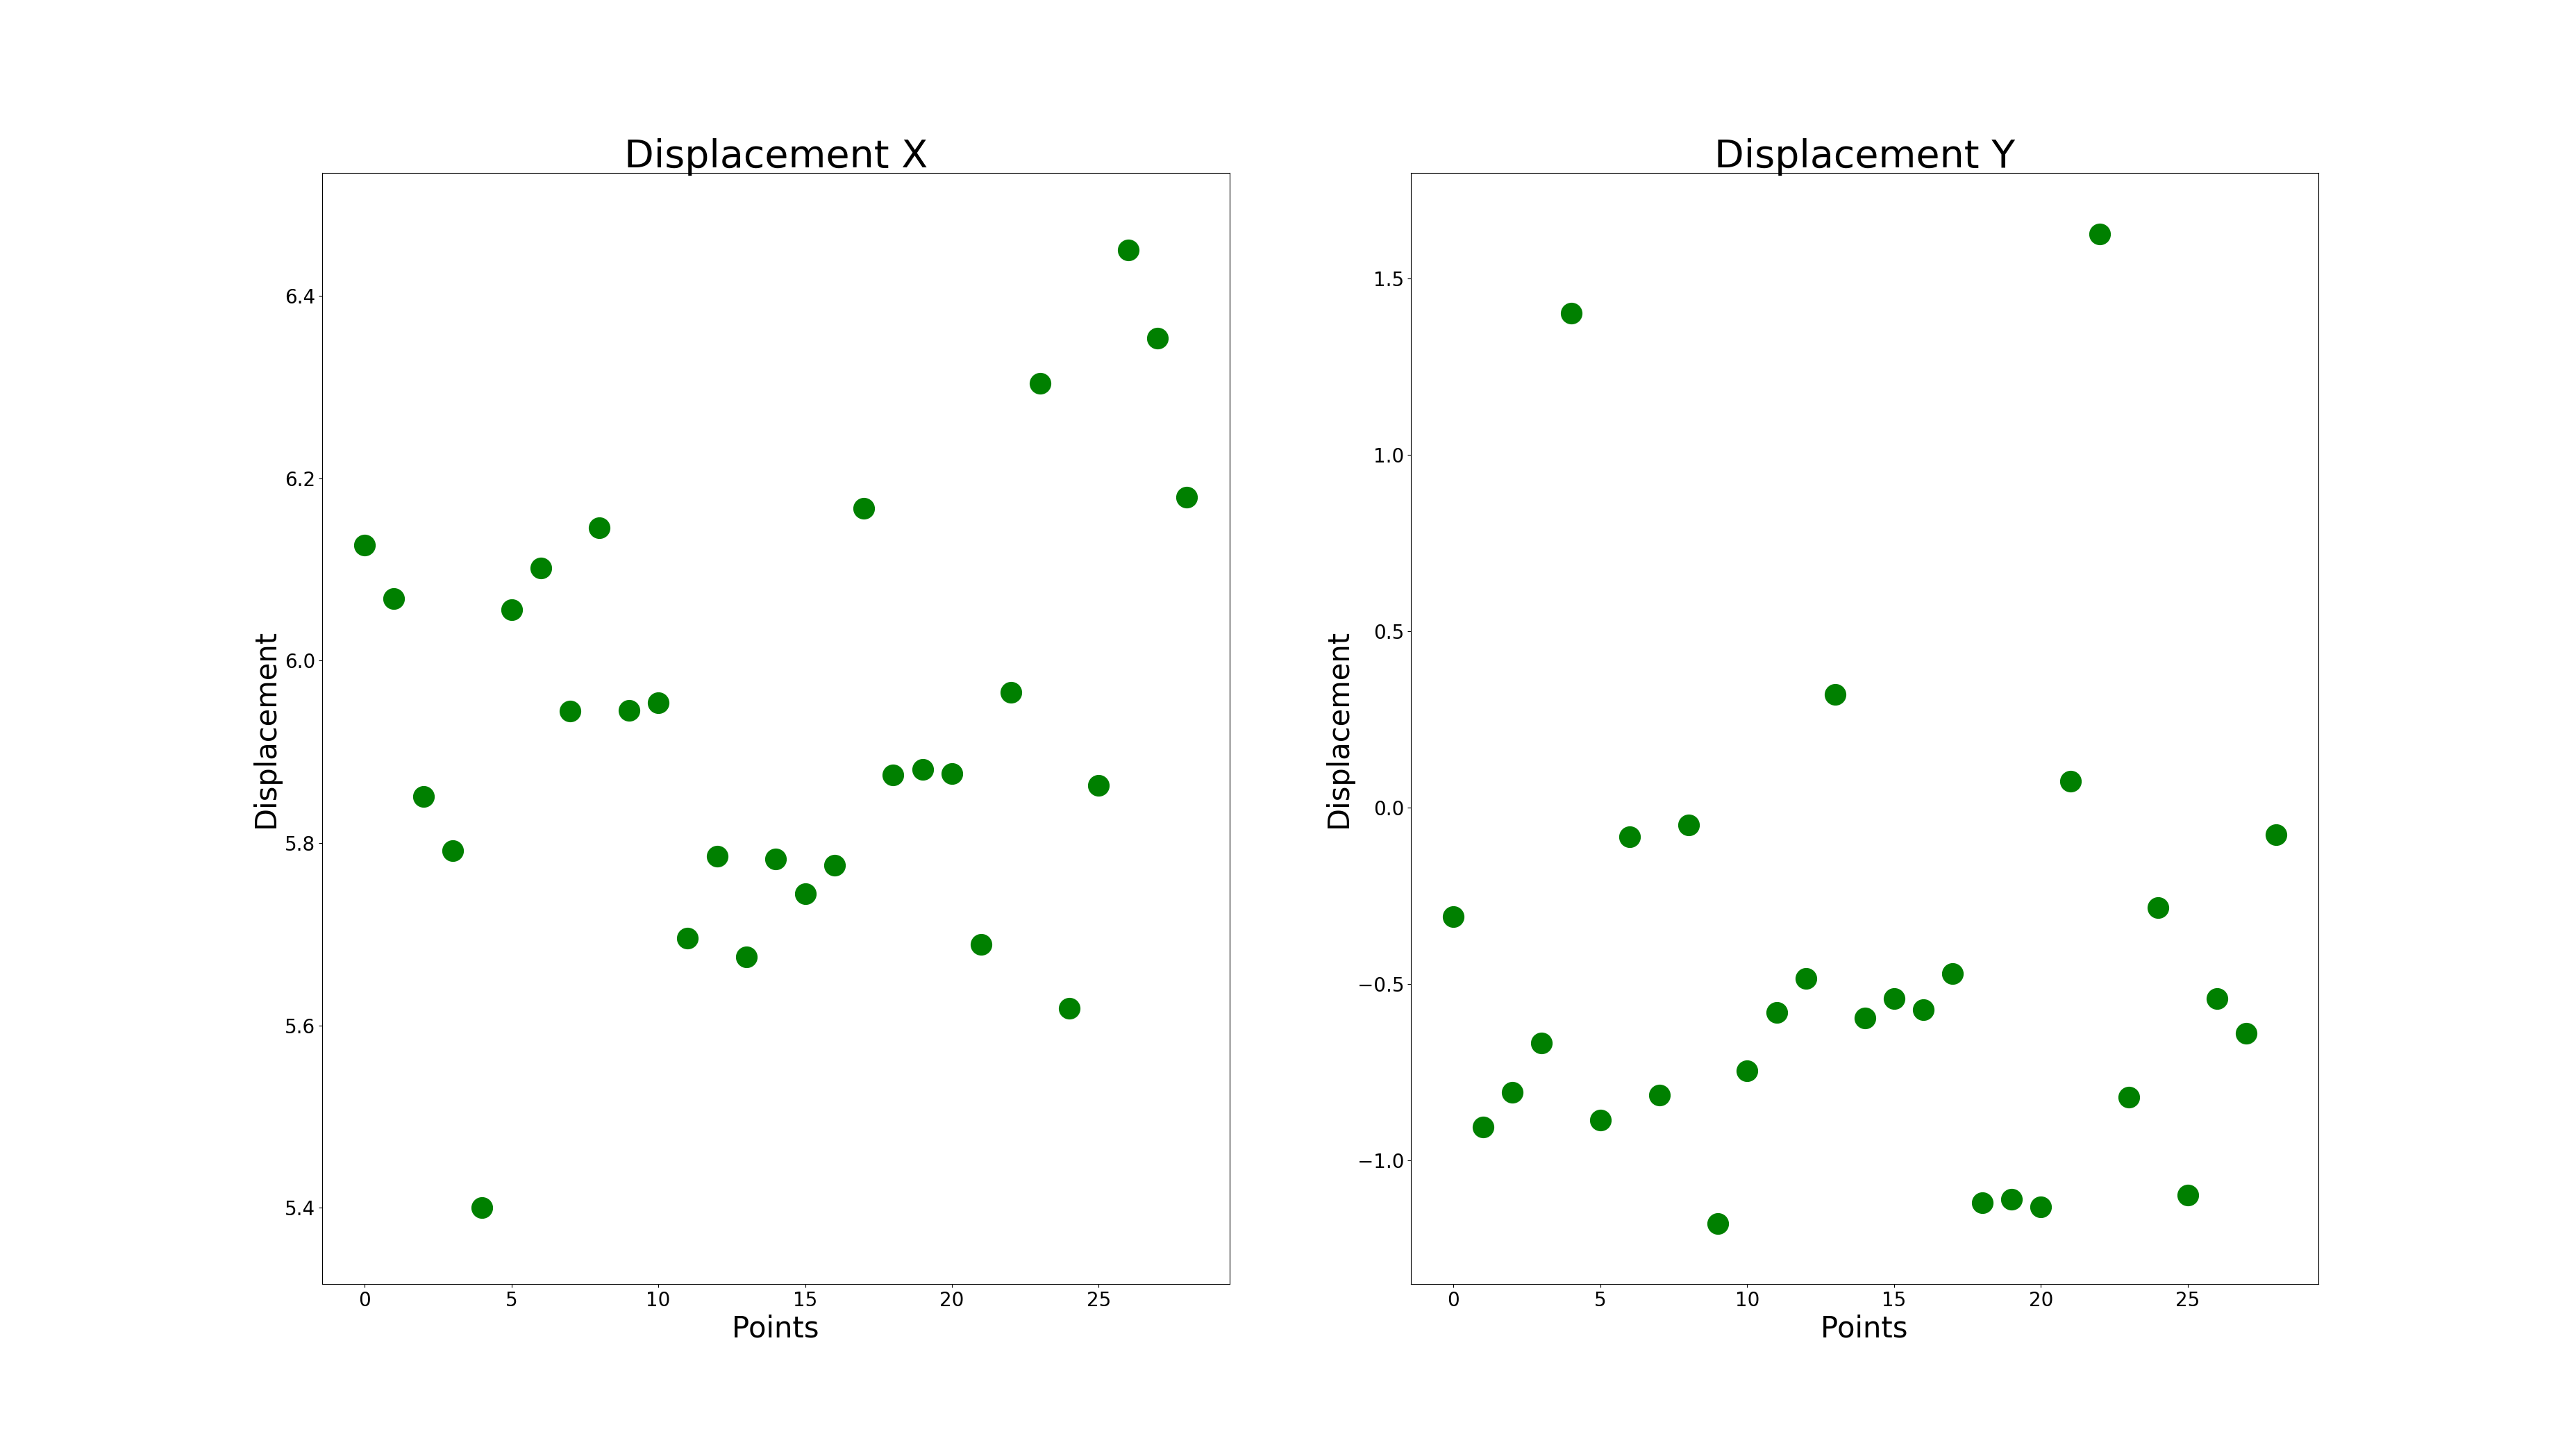
\includegraphics[width=13cm]{implementation/figurePoints.png}}\\
\caption{Different preprocessings.}
\label{motion3}
\end{figure}


Next we erased this points, we compute the motion as the median of all the contibutions displacement vectors. The scale change is computed as follows: for each pair of points, a ratio between current point distance and previous point distance is computed, bounding box scale change is defined as the median over these ratios. 

At this point, we have an implementation of the tracking algorithm given a set of bounding boxes. Nevertheless, we notice running our algorithm on the dataset, that the bounding box could compute the motion of the assigned pedestrian including the points belonging to another pedestrian who appears also in the bounding box and this interaction will cause a wrong estimation of the movement of the target and eventually the pedestrian will not be embedded by the bounding box. So, we need a mechanism to detect this fails, therefore we studied how the motion algorithm behaves in these situations. When it has got a trajectory without crossing with other pedestrian, the vertical and horizontal displacement behave like a damping sine wave   ( or amplified sine wave )   and the increment respect the previous displacment is small. We can observe this process in figure \ref{motion2Correct}.




\begin{figure}[H]
		
\centering

\subfigure[Trajectory.]{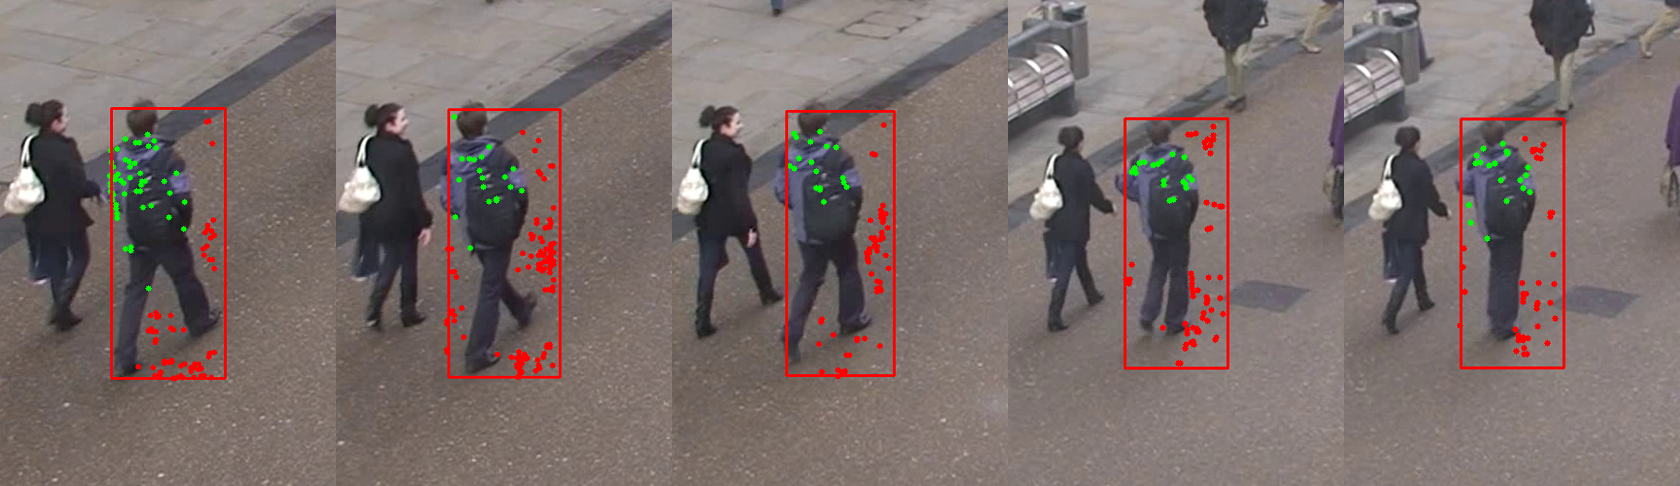
\includegraphics[width=15cm]{velocidadas/tomeuPont.png}}\\
\subfigure[Plots movement.]{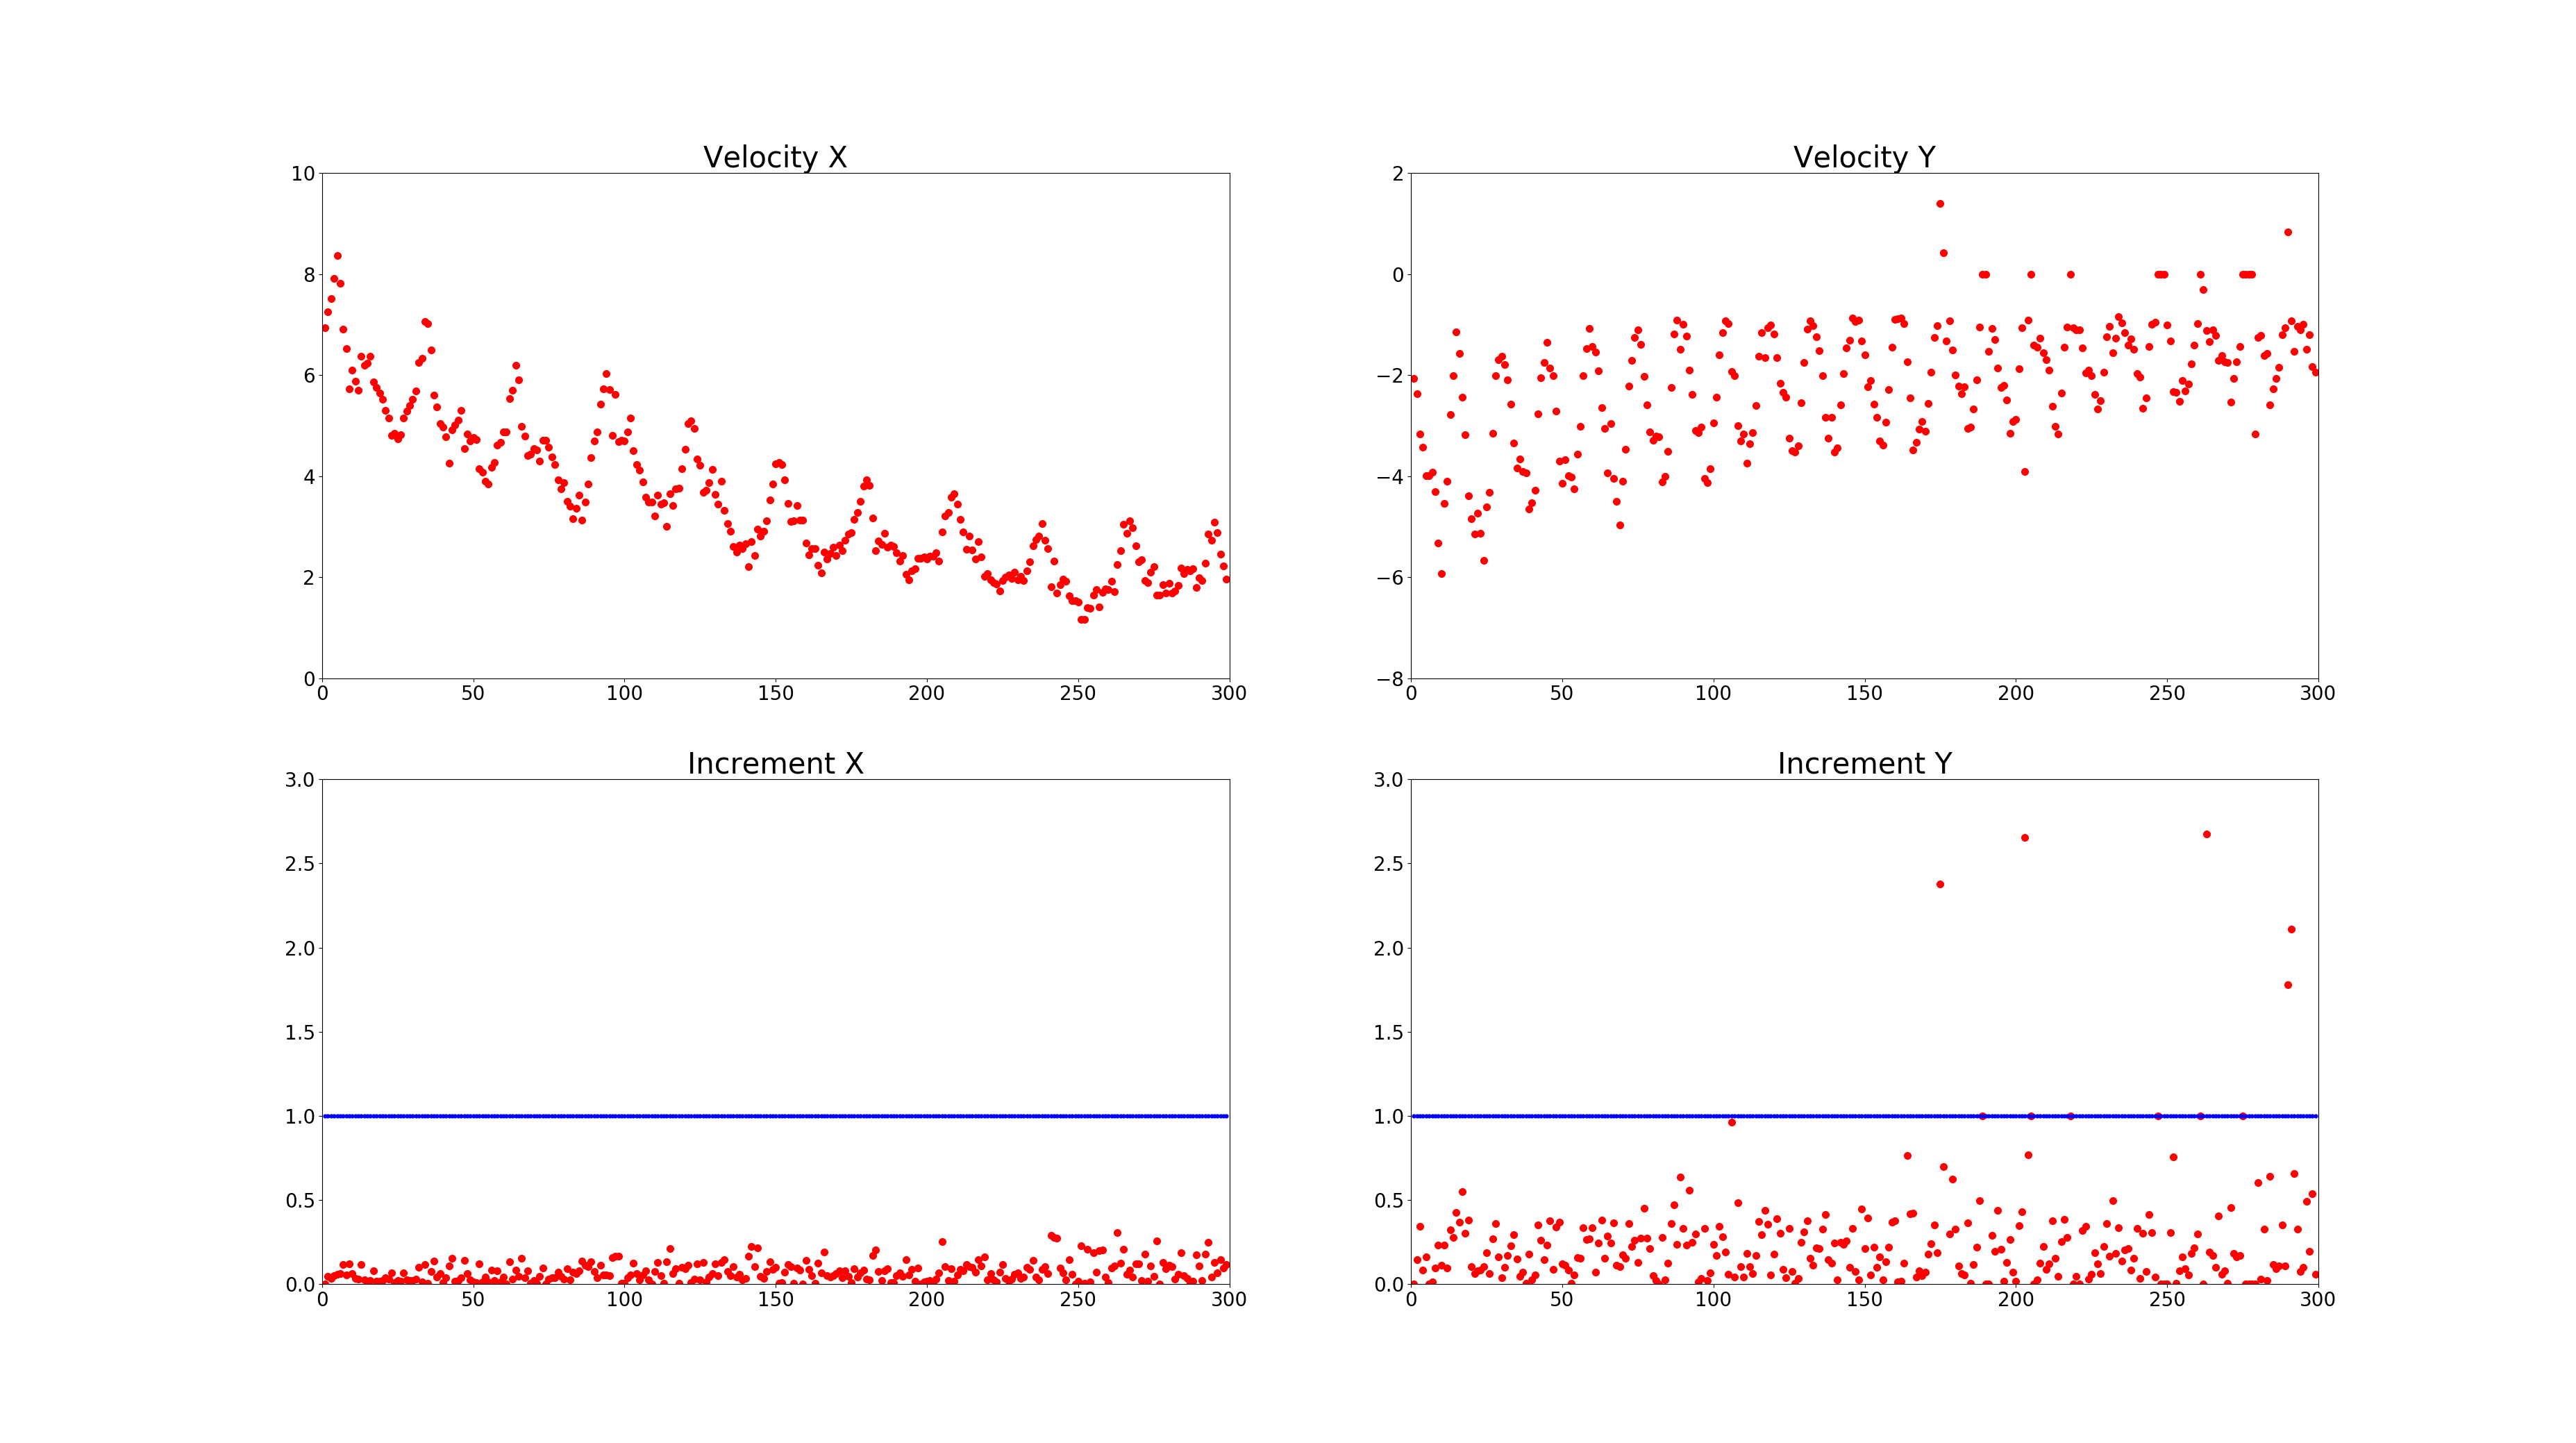
\includegraphics[width=16cm]{velocidadas/good_treshold.png}}\\
\caption{Regular trajectory.}
\label{motion2Correct}
\end{figure}


In contrast, when it crosses with another pedestrian, the displacement gets disrupt, then the normalized different with the previous displacement gets a high value, we can observe this process in figure \ref{motion2nocoorrect}. We set a threshold to notice this interference and delete this bounding box. We delete them from the current tracking execution, but we save the bounding box for following processings.

\begin{figure}[H]
		
\centering

\subfigure[Trajectory.]{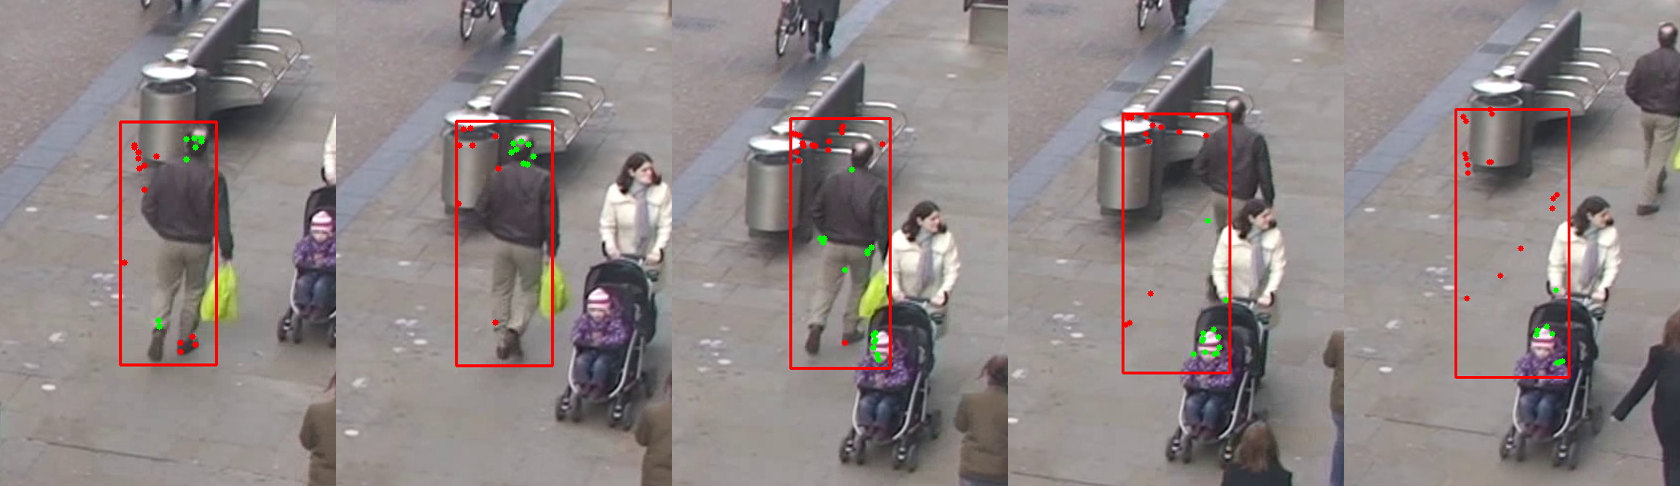
\includegraphics[width=15cm]{velocidadas/mateuPont.png}}\\
\subfigure[Plots movement.]{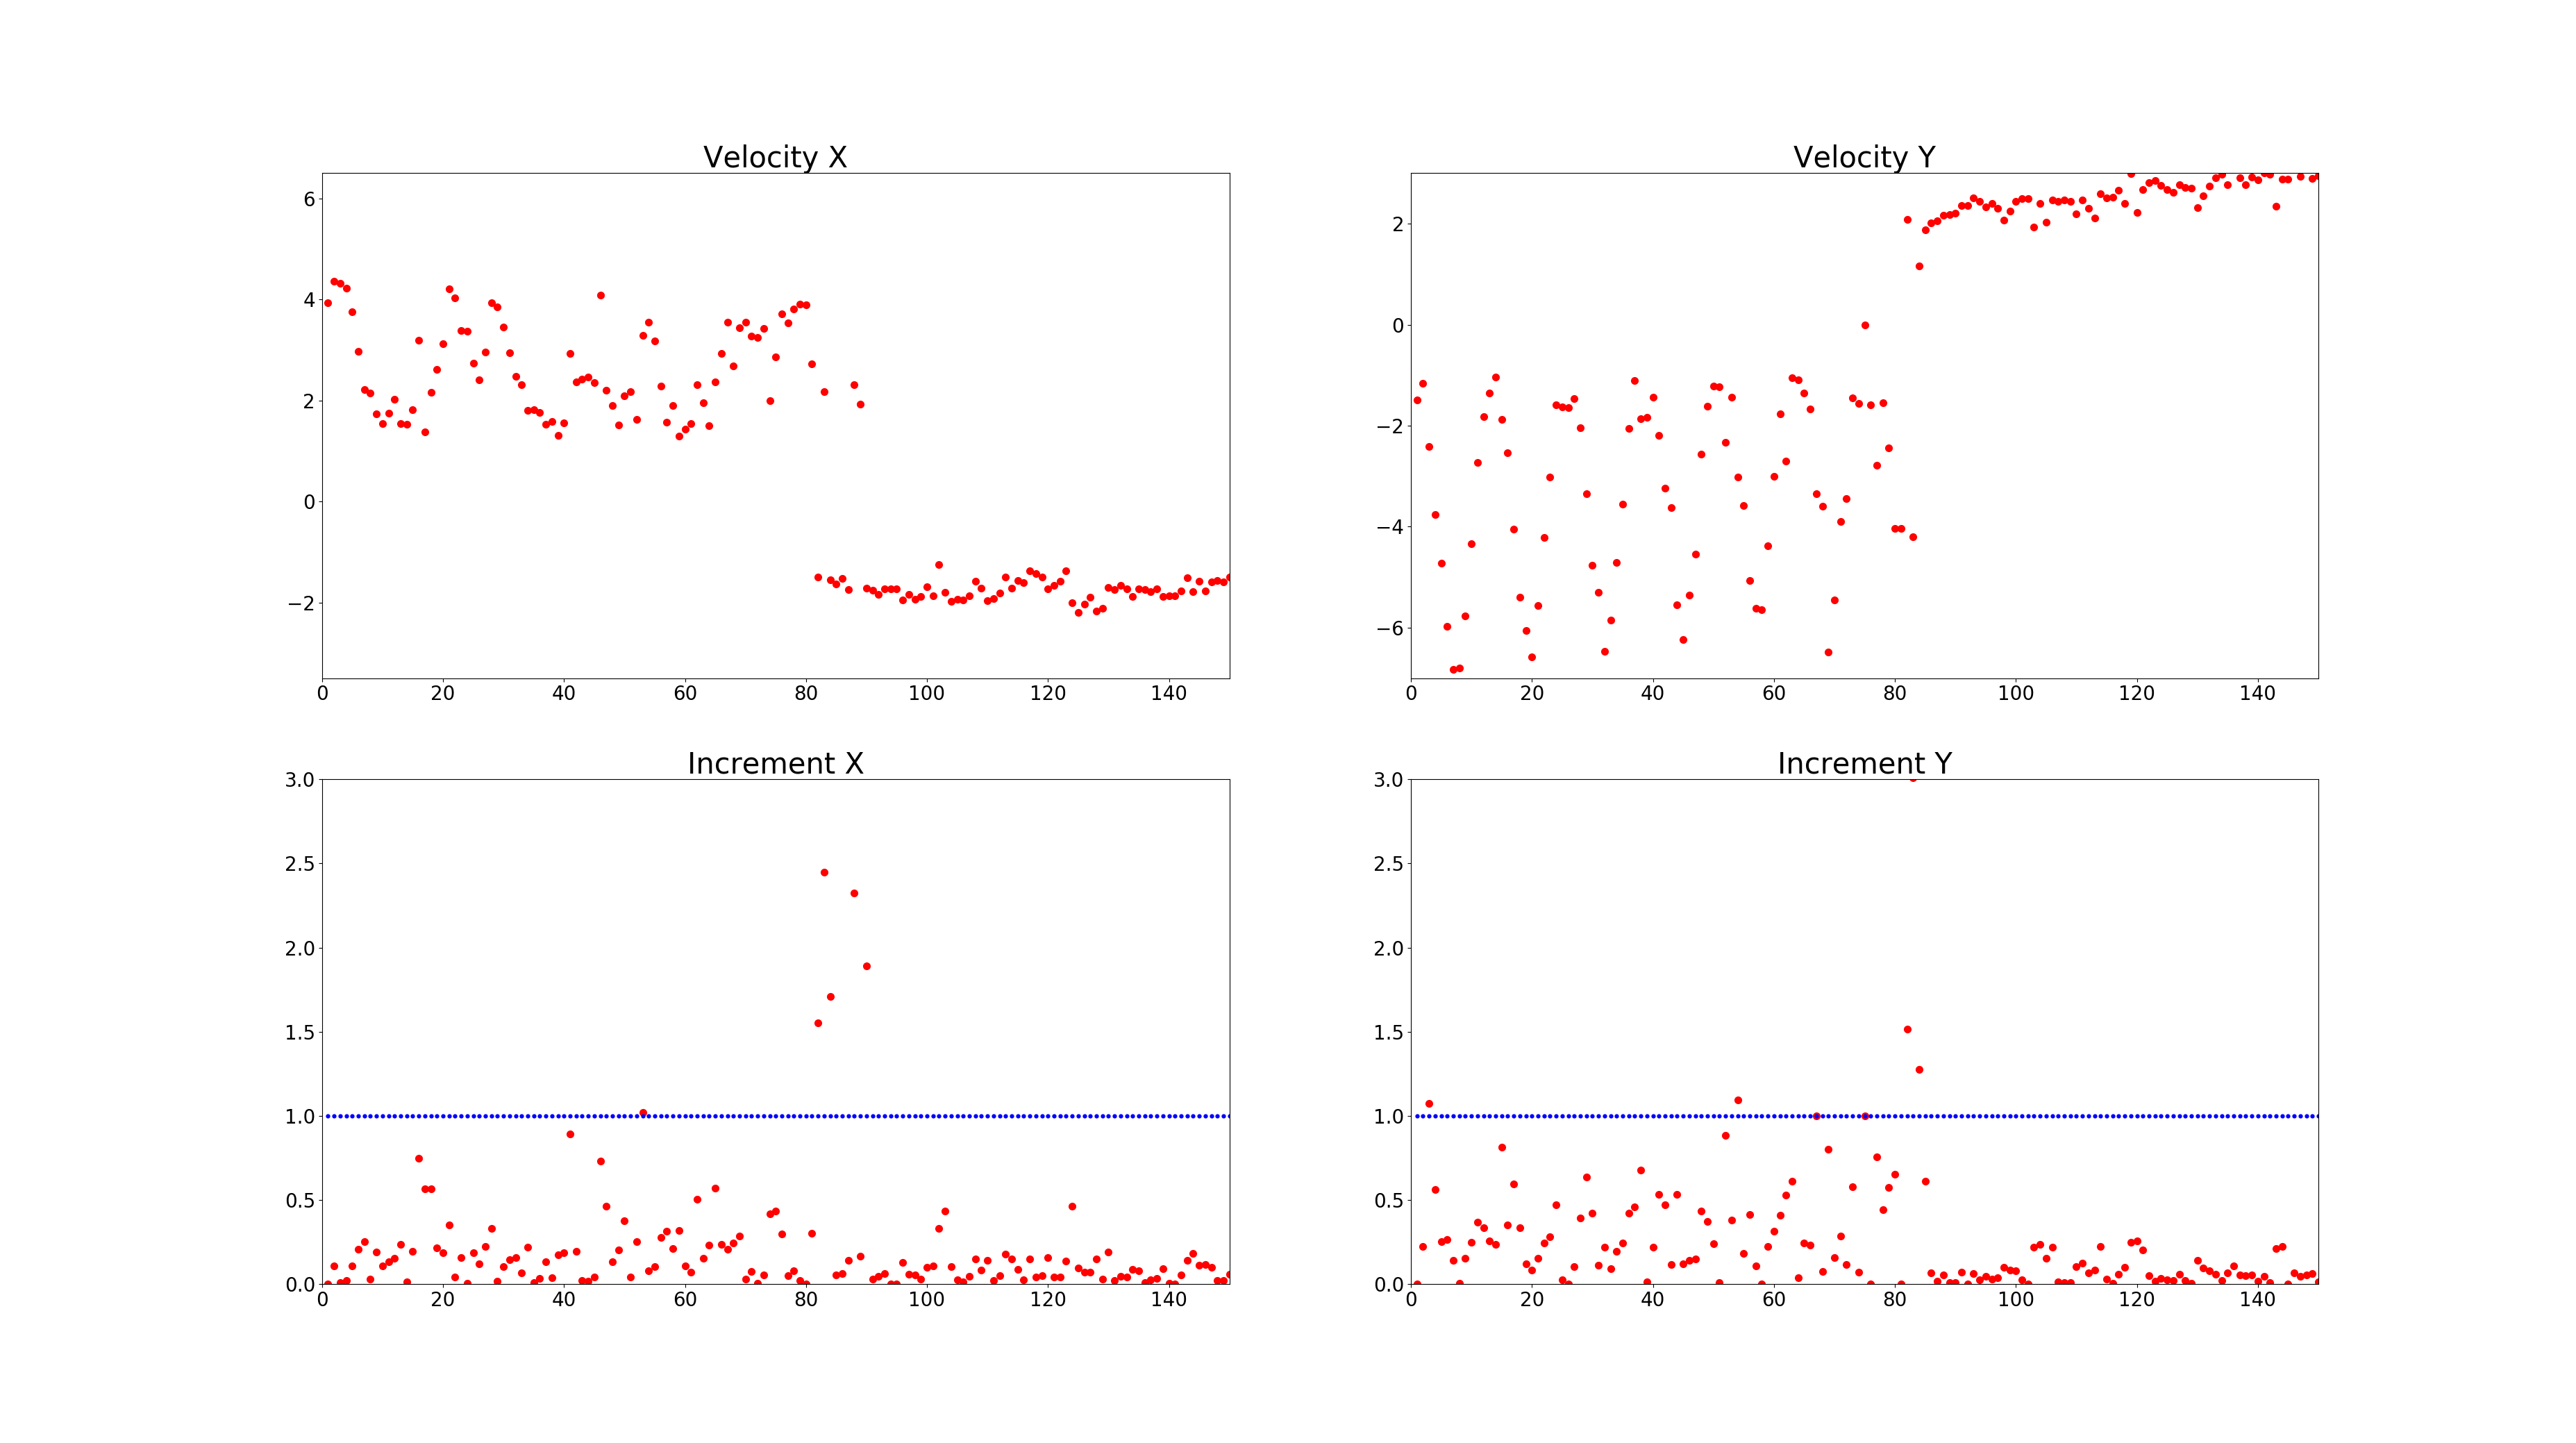
\includegraphics[width=16cm]{velocidadas/bad_threshold.png}}\\
\caption{Wrong trajectory.}
\label{motion2nocoorrect}
\end{figure}





\subsection{Data association}


Once we computed the trajectories, in the next iteration we might have to add a detection, so we need a module to combine these trajectories with detections. So, for each pedestrian we distinguish three situations:

\begin{itemize}



\item \textbf{Situation 1}, the tracket has got a nearby detection, then the detection replace the tracket bounding box. This is what is called spatio-temporal constraint.

\item \textbf{Situation 2}, the tracket has not got a nearby detection, then the bounding box tracket continues.

\item \textbf{Situation 3}, the pedestrian has not got a tracket but has got a detection. In this case we need to decided whether this pedestrian is new in the scene or it has been seen before ( it is a lost tracket ).

\end{itemize}

We can observe the procedure for situations number one and two in the figure \ref{data1}, in green colour we can observe the detections and in blue colour the trackets. We defined nearby as the distance between the centres of the boundings boxes, this distance has to be lower than a threshold to be consider nearby. 

\begin{figure}[hptb]
\centering         
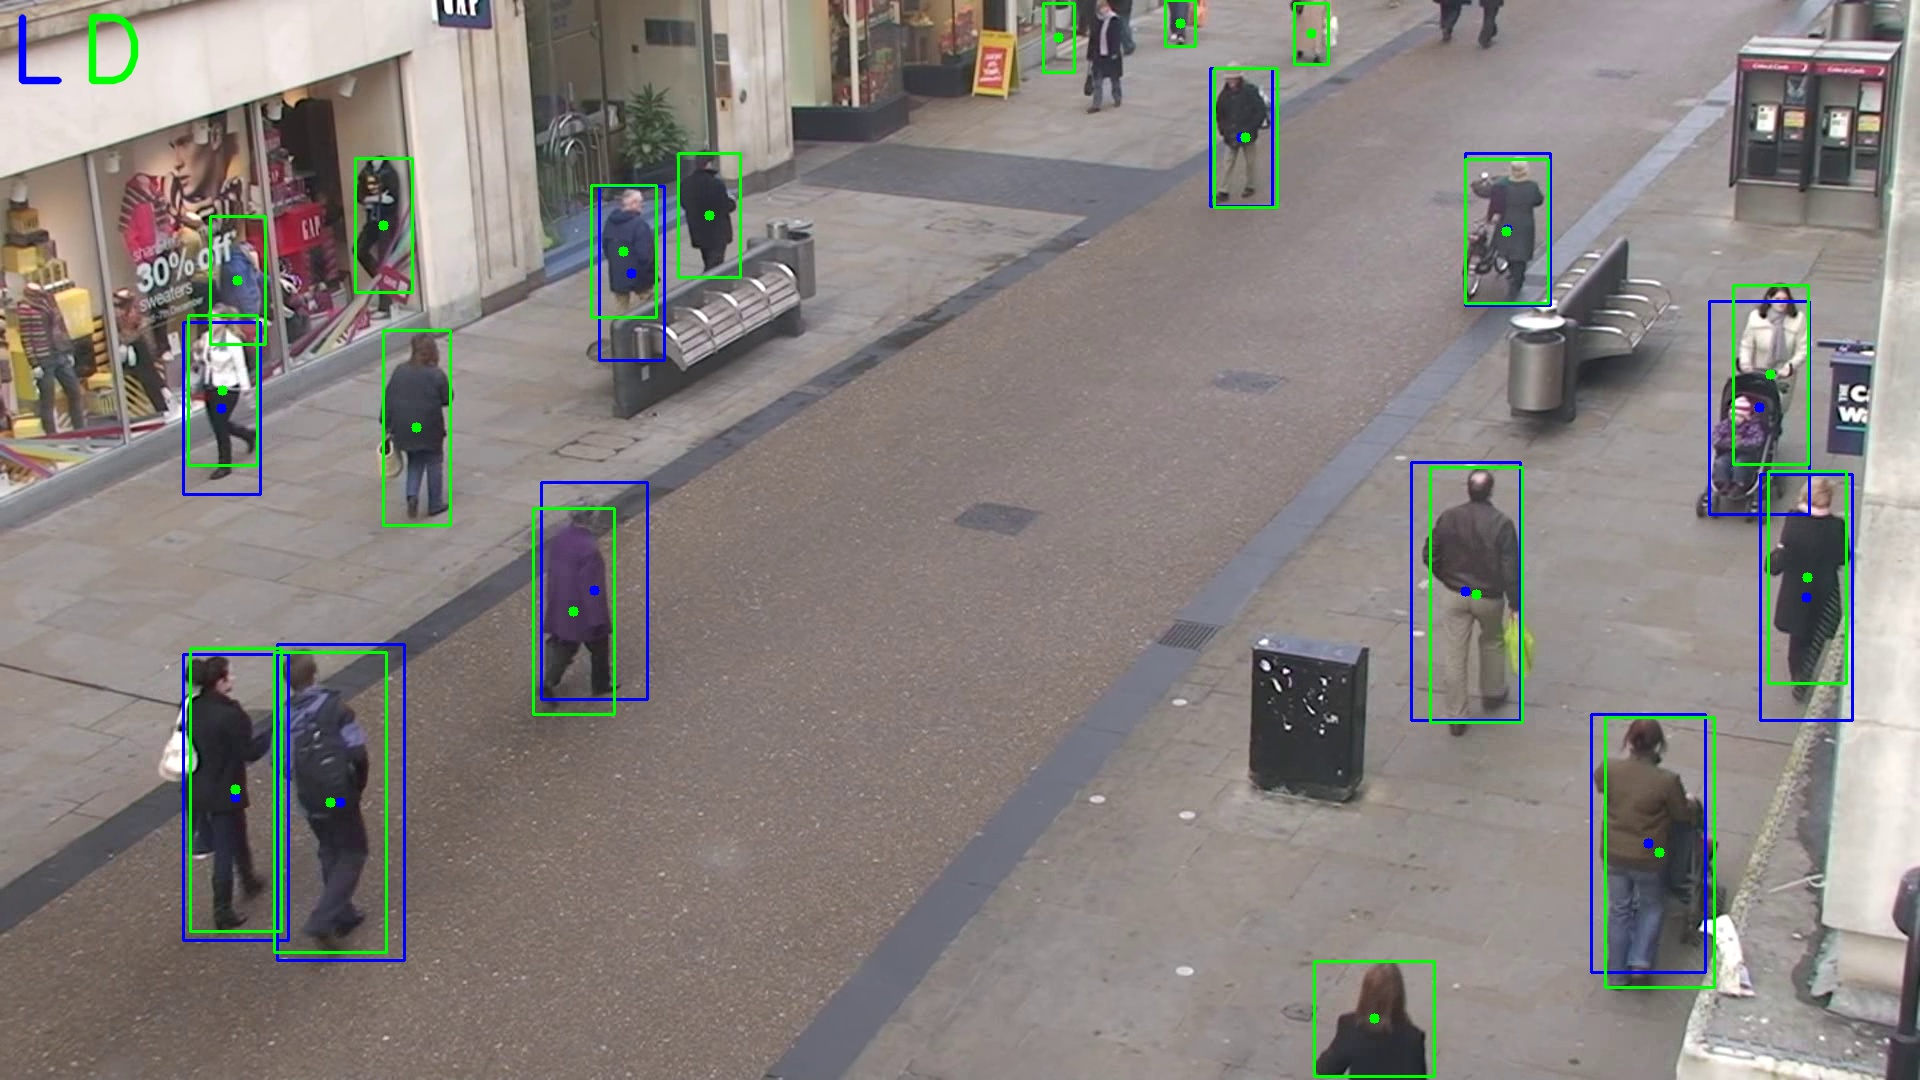
\includegraphics[width=12cm]{lucasKanade/dataAssociation.jpg}
\caption{Spatio-temporal data association.} \label{data1}
\end{figure}


As we stated, in situation number three, we might delete some tracking bounding box, like we explained in section \ref{mott} and get a new detection that it might belong to the same identity, we need a mechanism to preserve the identity of the pedestrians. In an early version of this algorithm we consider those detections as new, and we assign it a new identity.





\subsubsection{Siamese Network}


To mantain the identity of the pedestrian we need a mehtod to compare miss trackets with no associated detections. So, we decided to solve it with deep learning techniques, the convolutiona neural networks that we considered are the following:


\begin{itemize}

\item \textbf{Siamese network: Joint data input}, according to the literature this architecture gives the best results compared with the other topologies. The input of the network is aa concatenation of the two images and the network proces together.

\item \textbf{Siamese network: Cost function}, this is based on the idea of deep learning as feature extractor and top layers as classifier. Two branches that share parameters process the images and classify it.

\item \textbf{Siamese network: In-network}, this is a mix of the previous models, where the information of the convolutional layers merges at some point before the classifier.

\item \textbf{Feature extractor with cosine distance}, we used well-known architectures for image classification to extract features from the images and then compare those features with the cosine distance.

\item \textbf{Famous network fine-tuned}, we extract features for each image with a well-known architecture and merge it with a fully connected layer.

\end{itemize}

We can observe this architectures in the figure \ref{siameseData1}.

\begin{figure}[H]
		
\centering

\subfigure[Cost function.]{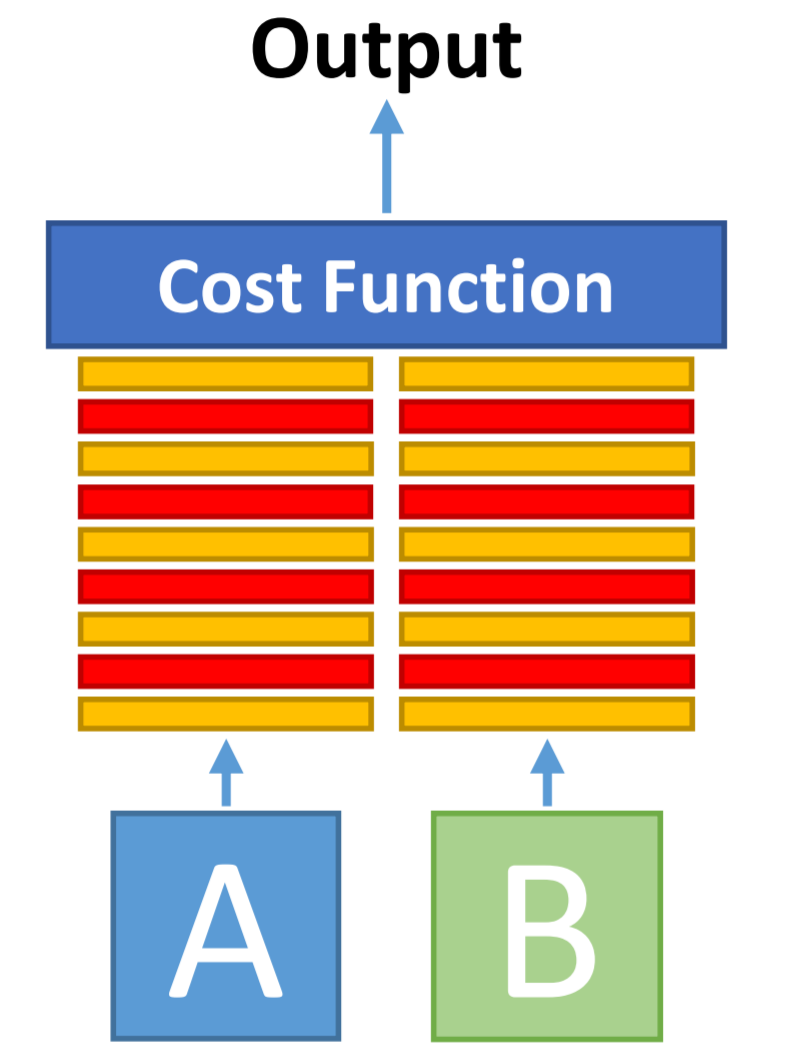
\includegraphics[width=2.7cm]{siamese/retall1.png}}
\subfigure[In-network.]{\includegraphics[width=2.7cm]{siamese/retall2.png}}
\subfigure[Joint data input.]{\includegraphics[width=2.7cm]{siamese/retall3.png}}
\subfigure[Features with cosine distance.]{\includegraphics[width=2.7cm]{siamese/cosineDistance.png}}
\subfigure[Cnn fine-tuned.]{\includegraphics[width=2.7cm]{siamese/retall2cnnMAss.png}}\\


\caption{Siamese CNN topologies.}
\label{siameseData1}
\end{figure}


%The base network has the following characteristic, several convolutional layers followed by max pooling, and in the end with a fully connected layer. We used the binary cross entropy as a loss, we tried with the contrastive divergence but it did not converge. As optimizer we used Adam, even though it has a mechanism to decrease the learning rate, we add a exponential decay, it speed up the convergence. To initialize the wrights we used He. inizialization, as activation function we used ReLu, in adition we inizializate the biases with the value of $0.1$, in this way we avoid the dead neurons at the begining. We make use of batch normalization to normailize the ouput of each layer. Also we use Dropout in the fully connected layer to avoid overfitting. In the junction between the convolutional layers and the fully connected historically, a flatten mechansihm of the tensor has been used, but it increases dramatically the number of neurons in the fully connected layer, and it shows problems to converge, from the publication of InceptionV3 it appears with a Global Average pooling, it computes the spatial average of each layer of the tensor, reducing the number of parameters.

The main characteristics of the trained networks are the following:

\begin{itemize}

\item \textbf{Loss}, we used the binary cross entropy as a loss, we tried with the contrastive divergence but it did not converge.

\item \textbf{Optimizer}, As optimizer we used Adam, even though it has a mechanism to decrease the learning rate, we add a exponential decay, it speed up the convergence

\item \textbf{Activation}, we used ReLu. Currently, there other activations functions, but ReLu has been stablished as the reference.

\item \textbf{Inizialization}, To initialize the wrights we used He. inizialization, as activation function we used ReLu, in adition we inizializate the biases with the value of $0.1$, in this way we avoid the dead neurons in the firsts iterations.

\item \textbf{Batch normalization}, We make use of batch normalization to normailize the ouput of each layer.

\item \textbf{Regularization}, we use Dropout in the fully connected layer to avoid overfitting.


\item \textbf{Final layers}, In the junction between the convolutional layers and the fully connected historically, a flatten mechansihm of the tensor has been used, but it increases dramatically the number of neurons in the fully connected layer, and it shows problems to converge, from the publication of InceptionV3 it appears with a Global Average pooling, it computes the spatial average of each layer of the tensor, reducing the number of parameters. Also we used the Spatial pyramid pooling layers

\begin{figure}[H]
		
\centering

\subfigure[Flatten.]{\includegraphics[width=4.5cm]{siameseDev/flatten2.png}}
\subfigure[Global average pooling.]{\includegraphics[width=4cm]{siameseDev/globalPooling.png}}
\subfigure[Spatial pyramid pooling.]{\includegraphics[width=4cm]{siameseDev/spp2.png}}\\



\caption{Final layers.}
\label{siameseData2}
\end{figure}


\item \textbf{Output}, We did not use softmax as ouput, we only used one neuron with sigmoid activation, in this way the output is constrainet between $0$ and $1$.



\end{itemize}

  

We developed our models in a VGG way, stacking  several convolutional layers and finishing it with a fully connected layers. We started with a few convolutional layers and added more till we reach an overfitting condition, this conditional will manifest when adding more layers the score on the test set decline. We started with $3$ and we end up with $7$ convolutional layer as best performance.

For the dataset, it does not exist a prominent dataset in the field, so we decided to use the MOT16 ground truth as dataset to adapt the domain. In order to do so, we extract the detections with their identities, and then for each identity we selected all possible random pairs and for the negative set we selected two random identites. The negative dataset is much bigger than the positive dataset, so we limited it to have a balanced dataset. The problem with the MOT16 dataset, is that the ground truth was built with the detections of a classifier and there is not a human intervention, resulting in a messy ground truth. We inspected the dataset and around the $70 \%$ of the dataset was wrong, there are a lot of oclussion in detection resulting in erronous pairs, pairs are not matching with the same identity.

Then, we decided to discard the MOT16 dataset an use the TownCenter dataset \cite{townCenter} from the University of Oxford. We have got $29824$ positive and negative pairs, then a dataset of $59648$ image pairs. We split the dataset between training and validation set, $80 \%$ and $20 \%$ respectively. For testing we selected a set of identities of the MOT16 dataset. To regularize and enlarge our dataset we added some data augmentation to our datase like we observe in figure \ref{msii1}. For each pair we added one transformation, so we double our dataset. We tried to apply all the transformation for each images but the dataset was too noisy and the network did not converge.






\begin{figure}[H]
		
\centering

\subfigure[Original image.]{\includegraphics[width=2cm]{dataAugmentation/resizedImage.jpg}}
\subfigure[Random image brightness.]{\includegraphics[width=2cm]{dataAugmentation/imageBrightnes.jpg}}
\subfigure[Random crop.]{\includegraphics[width=2cm]{dataAugmentation/imageRandomCrop.jpg}}
\subfigure[Vertical flip.]{\includegraphics[width=2cm]{dataAugmentation/imageVerticalFlip.jpg}}
\subfigure[Gaussian blur.]{\includegraphics[width=2cm]{dataAugmentation/imageGaussianBlur.jpg}}
\subfigure[Random shadow.]{\includegraphics[width=2cm]{dataAugmentation/imageRandomShadow.jpg}}


\subfigure[Zoom in.]{\includegraphics[width=2cm]{dataAugmentation/imageZoomIn.jpg}}
\subfigure[Rotation and translation.]{\includegraphics[width=2cm]{dataAugmentation/imageTransormed.jpg}}
\subfigure[Zoom out.]{\includegraphics[width=2cm]{dataAugmentation/imageZoomOut.jpg}}
\subfigure[Gaussian noise.]{\includegraphics[width=2cm]{dataAugmentation/imageNoiseGaussian.jpg}}
\subfigure[Opposite vignetting.]{\includegraphics[width=2cm]{dataAugmentation/imageBLURcenter.jpg}}
\caption{Data augmentation.}
\label{msii1}
\end{figure}

We trained all the models and obtained a graphs like the figure \ref{lossesSiam}, we observe that the network converge, it decreases the loss and increases the accuracy, also we observe that tests plots are a little bit noisy, but we considered that regularization techniques are enough.

\begin{figure}[H]
		
\centering

\subfigure[Losses.]{\includegraphics[width=7.5cm]{siameseDev/loss.png}}
\subfigure[Accuracy.]{\includegraphics[width=7.5cm]{siameseDev/accuracy.png}}\\

\caption{Results training.}
\label{lossesSiam}
\end{figure}



Finally, we can observe the comparision using the CMC measure in the figure \ref{lossesSiam2}, we can observe that the siamese with less layers than bigger models Incpetion perform better, this remarks the idea of training jointly the feature extractor and the classifier and the need of task specific networks. Also, the siamese network with the configuration Joint data input, outperforms the other siamese networks.




\begin{figure}[H]
		
\centering

\subfigure[CMC plot.]{\includegraphics[width=7.5cm]{siameseDev/cmcPlots2.png}}
\subfigure[Performance-timing comparision.]{\includegraphics[width=7.5cm]{graphicsRearrange/siameseGraph/siameseModels.png}}\\

\caption{Comparision of the systems.}
\label{lossesSiam2}
\end{figure}





\section{Datasets and evaluation procedures}

Next we explain the datasets and measures utilized in this thesis.

\subsection{Datasets for object detection}

This section describes the most common datasets used in object detection tasks. Throughout the history of computer vision research datasets have played a critical role.  They not only provide a means to train and evaluate algorithms, they drive research in new and more challenging directions. In order to accomplish this, they provide:


\begin{itemize}

\item a collection of challenging images and high quality annotation.

\item an standard evaluation methodology, so the performance of the algorithms can be compared. 


\end{itemize}



In the next subsections, we will explain the main datasets for object detection task.


\subsubsection{Pascal Visual Objects Classes}

The Pascal Visual Object Classes (VOC) challenge  \cite{voc07} is a benchmark in visual object category recognition and detection. Organised annually from 2005 to 2012, the challenge and its associated dataset has become accepted as one of the most benchmark for object detection. All the images are from the flickr consumer photographs website and annotated with the Mechanical turk tool.

The most popular editions of the challenge for object detection are those from years 2007 and 2012.

\subsubsection{VOC07}

%The VOC2007 dataset consists of annotated consumer photographs collected from %the flickr website. In addition, 

The challenge of the year 2007, it contains 10 thousand images in the trainval and test sets, with almost 12 thousand objects. This was one the first datasets for object detection before the era deep learning. Also, it is very useful for researchers, due it has 2.5 mean object per image and it is very challenging. In the figure \ref{data07} we can observe the distribution of images and objects instances. 

\begin{figure}[hptb]
\centering         
\includegraphics[width=0.7\linewidth]{datasets/log1.png}
\caption{Distribution of VOC07 dataset.} \label{data07}
\end{figure}



\subsubsection{VOC12}

The 2012's edition is also, one of the most used dataset in object detection tasks. It increases the volume of images of the 2007 edition up to 10 thousand images on trainval and test set and similar quantity of instances per image. 


\subsubsection{ImageNet}



ImageNet project \cite{imagenet} with the challenge ImageNet Large Scale Visual Recognition Challenge [ILSVRC] was the first large-scale database, temporally developed to supply the deep learning techniques, eager of feed with tons of images. ImageNet aims to populate the majority of the 80000 synsets of WordNet with an average of 500-1000 clean and full resolution images. The collection was based on the query of that words on several image search engines and human refined on the Amazon Mechanical Turk platform.

In 2016, the project collects more than 10 million of annotated images with 1000 classes. Although its main purpose is image classification, it has an object detection challenge with $200$ categories with over a 1 million images with objects annotated.







\subsubsection{COCO}

The Microsoft Common Objects in Context also known as COCO dataset \cite{coco}, is a dataset that address the three core research problems in scene understanding:


\begin{itemize}

\item detecting non-iconic views of objects, for many dataset most of the objects have an iconic representation, they appear unobstructed , near the center of the photo and with their canonical shape. So in this dataset, they included images to struggle the object recognition task, like objects in the background, partially occluded, amid clutter. Therefore, reflecting the composition of actual everyday scenes.

\item contextual reasoning between objects, nowadays natural images contain multiple objects, and their identity can only be solved using context, due to small size or ambiguos appearance in the image, so in this dataset, images contain scenes rather isolated objects. 

\item the precise 2D localization of objects, also the detailed spatial understanding of object layout will be a core component of an image understanding system, so this dataset struggle to do so.



\end{itemize}


So, the three main tasks of this challenge are object classification, object detection and semantic scene labelling. This dataset contains 91 object categories, with 2.5 million labelled object instances in 328 thousand images, labeled with the Amazon Mechanical Turk tool.

%
%\subsubsection{Dataset comparison}
%
%The table \ref{dataset0} summarizes the main statistics of the datasets and the figure \ref{diagrama2} the ratio of instances per images of the sets.
%
%The datasets from Pascal challenge are very useful to test object detection algorithms, their quantity is very handy ( a few thousands of images ) and contains a challenging quantity of objects per image, very interesting for the algorithms. But it little amount of images doesn't permit to train a network on this dataset, although it can be used to finetune the network.
%
%The datasets for the ImageNet challenge are not used to much in object detection tasks, it contains a few instances per image, this not encourage researcher to use it. Although, is very utilize to extract features and then finetune your net.
%
%
%The COCO datasets, is the most recent one, is the one focus on object recognition, and the detection suppose a challenge due the objects are in common places and are very challenging to detect. And it is very interesting to due of the quantity of instances per image.
%
%
%\begin{table}[H]
%\centering
%
%\begin{tabular}{lllll}
%                                 & \textbf{VOC07} & \textbf{VOC12} & \textbf{ImageNet [ 2014 ]} & \textbf{Coco [ 2015 ]} \\
%\textit{trainval set}            & 5011           & 11540          & 476688                     & 165482                 \\
%\textit{test set}                & 4952           & 10991          & 40152                      & 81434                  \\
%\textit{Number of classes}       & 20             & 20             & 200                        & 80                     \\
%\textit{Mean obj per image}      & 2.5            & 2.4            & 1.1                        & 7.2                    \\
%\textit{Number person instances} & 4690           & 8566           & -                          & 300000                
%\end{tabular}
%\caption{Datasets tables}
%\label{dataset0}
%\end{table}
%
%
%\begin{figure}[H]
%\centering         
%\includegraphics[width=0.7\linewidth]{datasets/genral3.png}
%\caption{Distribution of pascal.} \label{diagrama2}
%\end{figure}
%
%
%
%\begin{figure}[H]
%		
%\centering
%\subfigure[Pascal VOC.]{\includegraphics[width=5.2cm]{datasets/pascal.jpg}}
%\subfigure[ImageNet.]{\includegraphics[width=5.2cm]{datasets/imagenet.jpg}}
%\subfigure[COCO.]{\includegraphics[width=5.2cm]{datasets/coco.jpg}}
%
%\label{iconic}
%\end{figure}
%


\subsubsection{Dataset comparison}

%The table \ref{dataset0} summarizes the main statistics of the datasets and the figure %\ref{diagrama2} the ratio of instances per images of the sets.

The datasets from Pascal challenge are very useful to test object detection algorithms, their quantity is very handy ( a few thousands of images ) and contains a challenging quantity of objects per image, very interesting for the algorithms. But its little amount of images does not permit to train a network on this dataset, although it can be used to finetune the network.

The datasets for the ImageNet challenge are not used to much in object detection tasks, it contains a few instances per image, this not encourage researcher to use it. Although, it is very utilize to extract features and then finetune your net.


The COCO datasets, is the most recent one, is the one focus on object recognition, and the detection suppose a challenge due the objects are in common places and are very challenging to detect. And it is very interesting to due of the quantity of instances per image.


The COCO challenge contains 91 object categories with 82 of them having more than 5 thousand labeled instances. In total the dataset has 2.5 million labeled instances in 328 thousand images. In contrast to ImageNet dataset, COCO has fewer categories but more instances per category. Also, it has more instances per category than the VOC dataset. We can observe that difference in the chart \ref{instancesCategory}. This fact aid in learning detailed object models capable to chance the variability and also its 2D location.

\begin{figure}[H]
\centering         
\includegraphics[width=0.7\linewidth]{datasets/sdad2.png}
\caption{Distribution of pascal.} \label{instancesCategory}
\end{figure}

In addition, another prominent feature of the COCO over the other two, is the number of labelled instances per image which may aid in learning contextual information. This difference can be seen in \ref{instancesImage} chart.

%\begin{figure}[H]
%\centering         
%\includegraphics[width=0.7\linewidth]{datasets/instancesPerImage.png}
%\caption{Distribution of pascal.} \label{instancesImage}
%\end{figure}

Moreover, the COCO dataset uses images from non-canonical point view, allowing to the algorithm to be robust to everyday views. This feature can be observed in the plot \ref{iconic}, in this plot we can observe differences views of the same category. And clearly the coco's images is the most uni-conic representation.

\begin{figure}[H]
		
\centering
\subfigure[Pascal VOC.]{\includegraphics[width=5.2cm]{datasets/pascal.jpg}}
\subfigure[ImageNet.]{\includegraphics[width=5.2cm]{datasets/imagenet.jpg}}
\subfigure[COCO.]{\includegraphics[width=5.2cm]{datasets/coco.jpg}}
\caption{Distribution of pascal.} \label{iconic}

\end{figure}


Finally, the table \ref{dataset0} summarizes the main statistics of the dataset stated previously.

\begin{table}[H]
\centering

\begin{tabular}{lllll}
                                 & \textbf{VOC07} & \textbf{VOC12} & \textbf{ImageNet [ 2014 ]} & \textbf{Coco [ 2015 ]} \\
\textit{trainval set}            & 5011           & 11540          & 476688                     & 165482                 \\
\textit{test set}                & 4952           & 10991          & 40152                      & 81434                  \\
\textit{Number of classes}       & 20             & 20             & 200                        & 80                     \\
\textit{Mean obj per image}      & 2.5            & 2.4            & 1.1                        & 7.2                    \\
\textit{Number person instances} & 4690           & 8566           & -                          & 300000                
\end{tabular}
\caption{Datasets tables}
\label{dataset0}
\end{table}


\subsubsection{Evaluation of object detection algorithms}

In order to compare the performance of the different datasets, each challenges establish a clear measure. In this thesis, we used the interpolated average precision (AP), used in the Pascal VOC challenge (based on \cite{salton}).

For each class, the precision/recall curve is computed from a method's ranked output.

\begin{itemize}

\item Recall, is defined as the proportion of all positives examples ranked above a given rank.

\item Precision is the proportion of all examples above the rank which are from the positive class.

\end{itemize}


The AP summarises the shape of the precision/recall curve, and is defined as the mean precision at a set of eleven equally spaced recall levels [0,0.1,...,1]:

$$ AP = \dfrac{1}{11} \sum_{r \epsilon (0,...,1)} p_{interp}(r) $$

The precision at each recall level $r$ is \textit{interpolated} by taking the maximum precision measured for a method for which the corresponding recall exceeds $r$:

$$ p_{interp}(r) = max_{\hat r: \hat r>r} p( \hat r)$$

The authors justified this measurement as a way to reduce the impact of the 'wiggles' in the precision/recall curve, caused by small variations in the ranking of examples. In the figure \ref{diagramaI}, we can observe this effect on the curve.

\begin{figure}[H]
\centering         
\includegraphics[width=0.7\linewidth]{evaluacionObject/interpol.png}
\caption{Comparision interpolated and normal curve.} \label{diagramaI}
\end{figure}


In addition, detections were assigned to ground truth objects and judged to be true/false positives by measuring bounding box overlap. To be considered a correct detection, the area of overlap $a_{0}$ between the predicted bounding box $B_{p}$ and ground truth bounding box $ B_{gt}$ must exceed 0.5 by the formula:


$$ a_{0} = \dfrac{area(B_{p} \cap B_{gt})}{area(B_{p} \cup B_{gt})} $$

where $B_{p} \cap B_{gt}$ denotes the intersection of the predicted and ground truth bounding boxes and $ B_{p} \cup B_{gt} $ their union. The treshold of 50 \%  was set deliberately low to account for inaccuracies in bounding boxes in the ground truth data. Multiple detections of the same object in an image were considered false detections.

Finally, we want to point out, even we don't take into account in our implementation,  setting the threshold IoU to a value of $0.5$ could cause misdetections of small objects \cite{imagenet}, they propose an adaptive setting of that threshold based on the size of the ground truth and so detect correctly small objects. In practice this change only affects $5.5\%$ of objects in the detection validation set.








\subsection{Datasets for multiple object tracking}

Evaluating and comparing multi-target tracking methods is not trivial for numerous resasons. 

\begin{itemize}

\item First, the perfect solution one aims to achieve is difficult to define clearly. Partially visible, occluded, or cropped targets, reflections, and objects that are very closely resemble targets; all impose intrinsic ambiguities, such that even humans may not agree on one particular ideal solution.

\item Second, a number of different evaluation metrics with free parameters and ambiguous definitions often lead to inconsistent quantitative results across the literature.

\item Finally, the lack of pre-defined test and training data makes it difficult to compare different methods fairly.

\end{itemize}


In contrast to other research areas in computer vision, still lacks large-scale benchmarks.

\subsubsection{PETS}

Targeted primarily at surveillance applications \cite{pets}. The 2009 version consisted of 3 subsets, S1 targeted at person count and density estimation, S2 targeted at people tracking, and S3 targeted at flow analysis and event recognition. In the \ref{petsExample} we can observe one image from this dataset.

\begin{figure}[H]
\centering         
\includegraphics[width=0.5\linewidth]{datasetTracking/View_001.jpg}
\caption{Example of Pets.} \label{petsExample}
\end{figure}

Even for this widely used benchmark, we observe that tracking results are commonly obtained in an inconsistent fashion: involving using different subsets of available data, different detection inputs, inconsistent model training that is often prone to over-fitting, and varying evaluation scripts. Results are thus not easily comparable \cite{mot}.


\subsubsection{MOT challenge}

The aim of the Multiple object tracking [MOT] is to standardize the use of multiple people trackings datasets, in order to do so, they solve the problems in this kind of dataset, explained above.


\subsubsection{Evaluation of multiple people tracking algorithms}

A critical point with any dataset is how to measure the performance of the algorithms. A large number of metrics for quantitative evaluation of multiple target tracking have been proposed. Choosing unique general evaluation is still ongoing. 

On the one hand, it is desirable to summarize the performance into one single number to enable a direct comparison. On the other hand, one might not want to lose information about the individual errors made by the algorithms and provide several performance estimates, which precludes a clear ranking.


We will explain two sets of measures that have established themselves in the literature the CLEAR metrics \cite{clear}, and a set of track quality measures \cite{wu}.

As in the object detection metrics, we can classify each tracket, whether it is a true positive, that describes an actual (annotated) target, whether the output is a false alarm ( or false positive, FP ). This decisions is typically made by the well-known thresholding measure of Intersection of the union [IoU]. Also a target that is mised by any tracker is a false negative.

Due to we are working with multiple object, we assume that each ground truth trajectory has one unique start and one unique end point, that is not fragmented. So we need to penalty re-identification. This is called, identity switch [IDSW], and it is counted as if a ground truth target $i$ is matched to track $j$ and the last known assignment was $ k = j$. The next figure summarizes the stated measures ( the grey area indicate the the matching threshold ).


\begin{figure}[H]
\centering         
\includegraphics[width=0.7\linewidth]{datasetTracking/trackins.png}
\caption{Example of measures.} \label{petsExample}
\end{figure}

Then after determining true matches and establishing the correspondandes it is now possible to compute the metrics over all the sequences.


The multiple object tracking accuracy [MOTA] \cite{clear} is perhaps the most widely used figure to evaluate a tracker's perfomance. The main reason for this is its expressiveness as it combines as it combines three sources of errors defined above:

$$ MOTA = 1 - \frac{\sum_{t} (FN_{t}+FP_{t}+IDSW_{t})}{ \sum_{t} GT_{t}}$$

where $t$ is the frame index and GT is the number of ground truth objects. This measures gives an indication of the overall performance.

The multiple object tracking precision [MOTP] is the average dissimilarity between all true postives and their corresponding ground truth targets. For bounding box overlap, that is computed as 

$$ MOTP =  \frac{\sum _{t,i} d_{t,i}}{ \sum_{t} c_{t}} $$

where $c_{t}$ denotes the number of matches in frame $t$ and $d_{t,i}$ is the bounding box overlap of target $i$ with its assigned ground truth object. Thereby gives the average overlap between all correctly matched hypotheses. So, the MOTP is a measure of localization precision.


As we have stated above, another metrics are the track quality measures. Each ground truth trajectory can be classified as mostly tracked (MT), partially tracked (PT), and mostly lost (ML). This is done based on how much of the trajectory is recovered by the tracking algorithm. A target is mostly tracked if it is successfully tracked for at least $80 \%$ of its life span, without consider if there are an identity switch. If a track is only recovered for less than $20 \%$ of its total length, it is said to be mostly lost (ML). All other tracks are partially tracked. Finally antoher quality measure is track fragmentations (FM), it counts how many times a ground truth trajectory is resumed at a later point.


\subsection{Datasets for pedestrian identification}

A number of datasets for image-based re-Identification have been released, and some commonly used datasets are summarized in table \ref{tableID}. 


\begin{table}[H]
\centering

\begin{tabular}{lllllll}
\textbf{Name}        & \textbf{Date} & \textbf{Images} & \textbf{IDs} & \textbf{Cameras} & \textbf{Label} & \textbf{Evaluation} \\
\textit{VIPeR} \cite{viper}      & 2007          & 1264                      & 632          & 2                & hand           & CMC                 \\
\textit{iLIDS}  \cite{lids}      & 2009          & 476                       & 119          & 2                & hand           & CMC                 \\
\textit{GRID}   \cite{grid}     & 2009          & 1275                      & 250          & 8                & hand           & CMC                 \\
\textit{CAVIAR} \cite{caviar}      & 2011          & 610                       & 72           & 2                & hand           & CMC                 \\
\textit{PRID2011} \cite{prod11}   & 2011          & 1134                      & 200          & 2                & hand           & CMC                 \\
\textit{WARD}   \cite{ward}     & 2012          & 4786                      & 70           & 3                & hand           & CMC                 \\
\textit{CUHK01} \cite{cuk1}     & 2012          & 3884                      & 971          & 2                & hand           & CMC                 \\
\textit{CUHK02}  \cite{cuk2}    & 2013          & 7264                      & 1816         & 10               & hand           & CMC                 \\
\textit{CUHK03}  \cite{cuk3}    & 2014          & 13164                     & 1467         & 2                & hand/DPM       & CMC                 \\
\textit{RAiD}  \cite{raid}      & 2014          & 1264                      & 43           & 4                & hand           & CMC                 \\
\textit{PRiD 450S} \cite{prid450}   & 2014          & 900                       & 450          & 2                & hand           & CMC                 \\
\textit{Market-1501} \cite{market} & 2015          & 32668                     & 1501         & 6                & hand/DPM       & CMC/mAP            
\end{tabular}
\caption{Statistical comparision datasets.}
\label{tableID}
\end{table}

Over recent years, progress can observed. The dataset scale is increasing. Many of these datasets are relatively small in size, especially those of early days, but recent datasets, such as CUHK03 and Market-1501, are larger. Both have over 1000 ID's and over 10000 bounding boxes, and both datasets provide good amount of data for training deep learning models. Second, the bounding boxes tend to be produced by pedestrian detectors, instead of being hand-drawn. Also, more cameras are used during collection, this helps to increase generalization. There are not a prominent dataset in the literature.

\subsubsection{Evaluation for pedestrian identification}

% http://ws680.nist.gov/publication/get_pdf.cfm?pub_id=50759

When evaluating identification algorithms, the cumulative matching characteristics (CMC) curve is usually used. CMC represents the probability that a query identity appears in differentsized candidate lists.

Formally \cite{faceCMC}, for each probe $p$ from $P_{G}$ we sort the similarity scores against gallery $G$, and obtain the rank of the match. Identification performance is then stated as the fraction of probes whose gallery match it at rank $r$  or lower. If the set of probes with a close match is:

$$ C(r) = \big\{ p_{j}: rank(p_{j}) \leq r  \bigr\} \hspace{0.3cm} \forall p_{j} \in P_{G}  $$

where the rank is defined as before. We now define the Cumulative match characteristic (CMC) to be the identification rate as a function of $r$:

$$ P_{I}(r) = \dfrac{\abs{C(r)}}{\abs{P_{G}}} $$

which we plot as the primary measure of identification performance. It gives an estimate of the rate at which probe images will be classified at rank $r$ or better. One drawback of the characteristics is its dependence on gallery size, $\abs{G}$.



\section{Experiments}

In this section, we will analyse the performance and the timings of our solution.

\subsection{Performance}

Using the code provided by the MOT16 challenge organization, we evaluate our solution, we evalauated the results of the version without re-identification module,\textit{v1}, the version with optical flow forward-bacward \textit{v2}, and the version with re-identification module and without forward-backwward method, also we compare with the state of the art, an anonymous submission to the MOT16's website. The resulsts are showed in table \ref{tableResults}.


%\begin{table}[H]
%\centering
%
%\resizebox{\textwidth}{!}{\begin{tabular}{llll|llll|llll|llll}
%            & \textbf{Rcll} & \textbf{Prcn} & \textbf{FAR} & \textbf{GT} & \textbf{MT} & \textbf{PT} & \textbf{ML} & \textbf{FP} & \textbf{FN} & \textbf{IDs} & \textbf{FM} & \textbf{MOTA} & \textbf{MOTP} & \textbf{MOTAL} & \textbf{FPS} \\
%\textit{v1} & 24.4          & 49.5          & 5.17         & 517         & 12          & 180         & 325         & 27502       & 83462       & 827          & 1053        & 9.8          & 69.3          & 6,5        & 17,2   \\
%\textit{v2} & 19.6          & 61.8          & 2.52         & 517         & 3           & 127         & 387         & 13373       & 88754       & 618          & 936         & 10.8          & 70.3          & 7.5  & 15,85                                        
%\end{tabular}}
%\caption{Results algorithm global.}
%\label{tableResults}
%\end{table}


\begin{table}[H]
\centering

\resizebox{\textwidth}{!}{\begin{tabular}{llll|llll|llll|llll}
              & \textbf{Rcll} & \textbf{Prcn} & \textbf{FAR} & \textbf{GT} & \textbf{MT} & \textbf{PT} & \textbf{ML} & \textbf{FP} & \textbf{FN} & \textbf{IDs} & \textbf{FM} & \textbf{MOTA} & \textbf{MOTP} & \textbf{MOTAL} & \textbf{FPS} \\
\textit{v1}   & 21.4          & 49.5          & 5.17         & 517         & 12          & 180         & 325         & 13339       & 78998       & 827          & 1053        & 9.8           & 69.1          & 6.5            & 18.2         \\
\textit{v2}   & 21.3          & 50.4          & 5.12         & 517         & 11          & 181         & 325         & 11212       & 75738       & 827          & 1056        & 9.7           & 67.3          & 6.1            & 9.0          \\
\textit{v3}   & 19.6          & 61.8          & 2.52         & 517         & 3           & 127         & 387         & 13373       & 78999       & 618          & 936         & 10.8          & 70.3          & 7.5            & 15.85        \\
\textit{SOTA} & -             & -             & -            & 517         & 92          & 219         & 206         & 5333        & 86795       & 391          & -           & 49.3          & 79.0          & -              & 0.8         
\end{tabular}}
\caption{Results algorithm global.}
\label{tableResults}
\end{table}

According to this results, we decided to do not use the forward-backward method, due for its high computation demands. Also, we observe the usage of a mechanism of re-identification increment the MOTA performance, so the overall performance of the detector, with the cost of increae the running time. This improvement come from the reduction in around $24 \%$ the identity switching (ID's) paramter.

Finally we can observe the results in all the sequences \ref{tableResultsSequences}, we get a MOTA of $10.8$ and a frame rate of $15.85$ FPS. 

\begin{table}[H]
\centering

\resizebox{\textwidth}{!}{\begin{tabular}{llll|llll|llll|llll}
                & \textbf{Rcll} & \textbf{Prcn} & \textbf{FAR} & \textbf{GT} & \textbf{MT} & \textbf{PT} & \textbf{ML} & \textbf{FP} & \textbf{FN} & \textbf{IDs} & \textbf{FM} & \textbf{MOTA} & \textbf{MOTP} & \multicolumn{1}{l|}{\textbf{MOTAL}} & \textbf{FPS} \\
\textit{02}     & 12.9          & 51.4          & 3.63         & 54          & 0           & 13          & 41          & 2181        & 15526       & 113          & 146         & 0.1           & 67.1          & \multicolumn{1}{l|}{0.7}            & 9.02         \\
\textit{04}     & 28.5          & 71.2          & 5.23         & 83          & 0           & 41          & 42          & 5495        & 33980       & 185          & 290         & 16.6          & 71.1          & \multicolumn{1}{l|}{17.0}           & 12.3         \\
05              & 30.9          & 42.4          & 3.41         & 125         & 3           & 43          & 79          & 28571       & 4713        & 83           & 109         & -12.2         & 67.8          & \multicolumn{1}{l|}{-11.1}          & 17.94        \\
09              & 38.7          & 68.6          & 1.78         & 25          & 1           & 19          & 5           & 932         & 3225        & 62           & 71          & 19.7          & 71.2          & \multicolumn{1}{l|}{20.9}           & 10.52        \\
10              & 5.4           & 62.4          & 0.62         & 54          & 0           & 4           & 50          & 404         & 11647       & 81           & 133         & 1.5           & 68.4          & \multicolumn{1}{l|}{2.1}            & 14.23        \\
11              & 19.7          & 65.6          & 1.05         & 69          & 0           & 16          & 53          & 948         & 7366        & 72           & 121         & 8.6           & 71.4          & \multicolumn{1}{l|}{9.4}            & 17.49        \\
13              & 6.2           & 34.9          & 1.75         & 107         & 0           & 9           & 98          & 1315        & 10743       & 32           & 59          & -5.6          & 67.1          & \multicolumn{1}{l|}{-5.4}           & 20.5         \\ \hline
\textit{Global} & 19.6          & 61.8          & 2.52         & 517         & 3           & 127         & 387         & 13373       & 88754       & 618          & 936         & 10.8          & 70.3          & 7.5                                 & 15.85       
\end{tabular}}
\caption{Results algorithm by sequences.}
\label{tableResultsSequences}
\end{table}

The algorithm gets the best performance on sequences with a fixed camera from an elevated view point like sequences $4$ and a low angle recording with a high frame rate and close targets like sequences $9,and 11$, but it fails in sequences with low frame rate like sequences $5$ and when the targets are away from the camera like $13$.


\subsection{Timing}


As we stated above the mean frame rate of the algorithm with the person re-identification mechanism is $15.86$. In figure \ref{timing1} we can observe a barplot of per frame time consumption of our algorithm.  We notice the peaks each $30$ frames, these belong to the execution of the siamese network and it depends on how many detections without assignment there are.

\begin{figure}[H]
\centering         
\includegraphics[width=0.9\linewidth]{graphicsRearrange/temps/timeGenral.png}
\caption{Barplot of the timming.} \label{timing1}
\end{figure}

Getting a zoom of the graph \ref{timing2}, we can observe when the object detector finishes, it is around the frame $75$, then the execution time of the algorithm decresases, the time of reading the frame remain constant, and the tracking gets a peark after the detection and afterwards decreae this is due it erase tracket with the lost mechanism. 

\begin{figure}[H]
\centering         
\includegraphics[width=0.9\linewidth]{graphicsRearrange/temps/timeSpecfici.png}
\caption{Zoom in of the barplot.} \label{timing2}
\end{figure}

To optimize our code we studied how to reduce the execution time of the tracking module, plotting the execution time against some dependent variables, in this case, the number of points and the size of the ROI, as we can observe in figure \ref{timing2}. We notice that the execution time is high correlated with the size of the pedestrian's ROI and not with the number of points. The main responsable is the OpenCV's routine \texttt{calcOpticalFlowPyrLK()}, but we could not modify this parameter, and reducing the number of points would have a remarkable importance in the execution time. 



\begin{figure}[H]
		
\centering

\subfigure[Points vs time.]{\includegraphics[width=7.2cm]{graphicsRearrange/points/points1.png}}
\subfigure[Size ROI vs time.]{\includegraphics[width=7.2cm]{graphicsRearrange/points/timss.png}}
\caption{Time versus points and size of the ROI.}
\label{timing2}
\end{figure}








\section{Conclusions}


In this thesis we studied deep learning techniques and their application in a tracking algorithm. We included an object detector and a person re-identification module based on those techniques and we implemented a tracking algorithm.

This tracking algorithm, takes the detections of the object detector and computes the optical flow on the sequences. When it misses some pedestrians it can preserve their identity with a person re-identification module.

Finally we evaluated our algorithm in a well-known challenge, MOT16, and analyses its performance and timing capabilties on it. The algorithms performs reasonably well in sequences of high frame rate and resolution, but in the opposite sequences, low frame rate and resolution the performance drop dramatically. This is happens beacause our algorithm rely on points with high texture, with a low resolution there are less points with this characteristics. Also, we have problems with people who wear low texture or are away from the camera, as we can oberve in figure \ref{Fails1}. The low frame rate, penalize the matching capabilites between frames, it produces wrong matches between images, therefore, wrong displacements.




\begin{figure}[H]
		
\centering

\subfigure[High texture person.]{\includegraphics[width=5cm]{changeCamera/tomeuTetx.png}}
\subfigure[Low texture person.]{\includegraphics[width=5cm]{changeCamera/donaTetx.png}}
\subfigure[Far away person.]{\includegraphics[width=5cm]{changeCamera/foto004.png}}
\caption{Differences texture examples.}
\label{Fails1}
\end{figure}








\subsection{Future work}


This is a first entrance on trackings algorithm, we have a resanoable results. We can add some details to improve our results.


\begin{itemize}

\item Port to C++. We used a srcipting programming languagge, if we switch to a compiled programing language we would increase the time perfomance.

\item GPU implementation. Computing displacement for each tracket could be computed in a parallel way. They are independent from each other and are a low demanding. 

\item Propbabilistic framework. Include bayesian filter techniques to increase perfomance.

\item Siamese architectures. Study new siamese architecture to increase the accuracy of this modeule, like inception stem of InceptionV3 or include the optical flow information in the neural network.

\item Data association. Use much confidence techniques to associate the detections, the current methods relay ond probablistic graphical models.

\end{itemize}

\bibliography{mybib}{}
\bibliographystyle{plain}







\end{document}
